\section{Base Te\'orica}\label{sec:base}

A base teórica é fundamental para se obter resultados satisfatórios, pois ela proporciona um sólido conhecimento sobre o tema em questão. Neste capítulo, são abordados diversos aspectos relevantes, incluindo métricas de erro e modelos regressivos de previsão. Essas métricas desempenham um papel crucial na avaliação e comparação dos modelos, permitindo uma análise precisa do desempenho de cada um. Além disso, os modelos regressivos de previsão são explorados, fornecendo insights valiosos sobre como essas técnicas podem ser aplicadas para realizar previsões com precisão. Compreender e dominar esses conceitos é essencial para se obter resultados confiáveis e embasar as próximas etapas do trabalho de pesquisa.

\subsection{M\'etricas de Avalia\c c\~ao de Modelos}\label{subsec:metrica}

A métrica de Erro Quadrático Médio (MSE) é amplamente utilizada no campo do aprendizado de máquina para avaliar a qualidade dos modelos de previsão. O MSE é calculado pela média da soma dos quadrados das diferenças entre os valores reais e os valores previstos,

\begin{eqnarray}
	MSE &=& \frac{1}{n} \sum_{i=1}^{n} (y_i - \hat{y}_i)^2 \label{eq:mse}
\end{eqnarray}

\noindent onde, $n$ representa o número de amostras, $y_i$ é o valor real correspondente à amostra $i$ e $\hat{y}_i$ é o valor previsto para a mesma amostra. O MSE é calculado como a média das diferenças ao quadrado entre os valores reais e os valores previstos.

A utilização do MSE fornece uma medida quantitativa da precisão do modelo, pois penaliza de forma mais significativa os erros maiores. Ao elevar as diferenças ao quadrado, a métrica enfatiza a importância de minimizar as discrepâncias entre os valores reais e os valores previstos. Dessa forma, quanto menor o valor do MSE, melhor é o desempenho do modelo em termos de previsão.

Portanto, o MSE é uma métrica fundamental para avaliar a qualidade dos modelos de previsão e é amplamente utilizada para comparar diferentes algoritmos e abordagens de aprendizado de máquina.

\subsubsection{Erro Quadr\'atico M\'edio Raiz (RMSE)}

O RMSE é uma métrica amplamente empregada na avaliação de modelos de previsão em séries temporais. Ele é calculado tomando a raiz quadrada do MSE, conforme segue,

\begin{eqnarray}
	RMSE &=& \sqrt{\dfrac{1}{n} \sum_{i=1}^{n} (y_i - \hat{y}_i)^2} \label{eq:rmse}
\end{eqnarray}

\noindent onde \eqref{eq:rmse}, $n$ representa o número de amostras, $y_i$ é o valor real correspondente à amostra $i$, e $\hat{y}_i$ é o valor previsto para a mesma amostra. O RMSE fornece uma medida da dispersão média entre os valores reais e os valores previstos pelo modelo.

Uma das vantagens de utilizar o RMSE é que, ao computar a raiz quadrada, o erro passa a ter a mesma escala da variável de interesse. Isso permite uma interpretação mais fácil dos resultados, sendo que um valor baixo de RMSE indica um bom desempenho do modelo, já que o erro se aproxima de zero.

O RMSE possui algumas características positivas. Ele penaliza de forma significativa os valores discrepantes, caso seja necessário para o modelo. Além disso, o erro resultante está nas mesmas unidades da série temporal, facilitando a interpretação. O RMSE pode ser considerado uma combinação das melhores características do MSE e do Erro Absoluto Médio (MAE).

No entanto, o RMSE também apresenta algumas desvantagens. Ele tem uma interpretabilidade reduzida, uma vez que os erros ainda são elevados ao quadrado. Além disso, o RMSE é dependente da escala dos dados, o que impede sua comparação direta com modelos de séries temporais que utilizam unidades diferentes.

Apesar das limitações, o RMSE é uma métrica amplamente utilizada para avaliar modelos de previsão em séries temporais. Ele fornece uma medida da dispersão média entre os valores reais e previstos, auxiliando na compreensão do desempenho do modelo e na comparação com outras abordagens.

\subsubsection{Raiz do Erro M\'edio Quadr\'atico Relativo (RRMSE)}\label{subsub:rrmse}

\noindent\textbf{Vantagens do RRMSE :}


Interpretação intuitiva: O RRMSE é expresso como uma porcentagem, o que facilita a compreensão da precisão relativa do modelo. Quanto menor o valor do RRMSE, mais próximas estão as previsões dos valores reais.
	
Considera a escala dos dados: O RRMSE leva em consideração a magnitude dos erros em relação aos valores de referência. Isso é especialmente útil quando os dados têm uma grande variação e escala, pois evita que erros de grande magnitude dominem a avaliação.
	
Comparação entre modelos e algoritmos: O RRMSE pode ser usado para comparar a precisão de diferentes modelos ou algoritmos em um problema de regressão. Ao calcular o RRMSE para cada modelo, é possível identificar aquele que apresenta melhor desempenho em relação aos valores reais.
	
Sensibilidade relativa a diferentes magnitudes de erro: O RRMSE captura erros relativos em diferentes magnitudes. Isso significa que ele é capaz de identificar discrepâncias proporcionais, independentemente do valor absoluto dos erros.


\noindent\textbf{Desvantagens do RRMSE:}


Sensibilidade a \textit{outliers}: O RRMSE pode ser influenciado por valores discrepantes nos dados. Se houver valores extremos que não representem a tendência geral, o RRMSE pode ser distorcido, pois considera a média dos valores reais na fórmula de cálculo.
	
Necessidade de uma linha de base adequada: O RRMSE requer uma linha de base apropriada para comparação. Isso significa que é necessário ter um valor de referência confiável ou um modelo de referência para calcular o RRMSE e interpretar os resultados corretamente.
	
Foco exclusivo na precisão relativa: O RRMSE se concentra exclusivamente na precisão relativa e não leva em consideração outras métricas de desempenho, como tempo de execução, complexidade do modelo ou outros aspectos específicos do problema em questão. Portanto, é importante complementar o uso do RRMSE com outras métricas relevantes,





\begin{eqnarray}
	\text{RRMSE} &=& \left(\frac{\text{RMSE}}{\text{Média dos Valores Reais}}\right) \times 100 \label{eq:rrmse}
\end{eqnarray}


\noindent onde RMSE representa o Erro Médio Quadrático e ``Média dos Valores Reais'' denota a média aritmética dos valores reais no conjunto de dados.

É essencial que sejam consideradas essas vantagens e desvantagens ao utilizar o RRMSE como métrica de avaliação. Além disso, é recomendado o uso de várias métricas em conjunto para obter uma visão mais completa do desempenho do modelo de regressão.



\subsubsection{Erro Absoluto M\'edio (MAE)}

O Erro Absoluto Médio (MAE) é amplamente utilizado como uma métrica para avaliar o desempenho de modelos de previsão. Em vez de calcular a média das diferenças entre os valores reais e previstos, o MAE calcula a média dos valores absolutos dessas diferenças, garantindo que os erros positivos e negativos não se anulem.

O MAE mede o desvio médio das previsões em relação aos valores reais e é uma métrica intuitiva e fácil de interpretar, representando a magnitude média dos erros em relação à escala dos dados. Por exemplo, um MAE de 2 significa que, em média, as previsões têm um desvio absoluto de 2 unidades em relação aos valores reais.

Uma das vantagens do MAE é a sua insensibilidade a valores extremos, pois trata os erros de forma absoluta. No entanto, como o MAE não considera a magnitude dos erros individuais, pode não refletir adequadamente a gravidade de desvios significativos em relação aos valores reais.

Para superar essa limitação, uma alternativa é o Erro Médio Absoluto Percentual (MAPE). O MAPE expressa o MAE como uma porcentagem em relação aos valores reais, proporcionando uma medida relativa de erro. Essa métrica é especialmente útil quando se deseja avaliar o desempenho de um modelo em relação à magnitude dos dados.

Em resumo, o MAE é uma métrica simples e fácil de interpretar, que mede o desvio médio das previsões em relação aos valores reais. O MAPE, por sua vez, fornece uma medida relativa de erro, expressa como uma porcentagem dos valores reais. A escolha entre essas métricas depende do contexto do problema e dos requisitos específicos de avaliação.

O cálculo do MAE é realizado utilizando o valor absoluto da diferença entre o valor real e o valor previsto, e em seguida, divide-se pela quantidade $n$ de amostras. Isso resulta no erro médio absoluto. A equação do MAE é dada por:

\begin{eqnarray}
	M A E &=& \dfrac{1}{n} \sum\left|y_i-\hat{y}_i\right|\label{eq:mae}
\end{eqnarray}

Sua interpretação é similar ao RMSE, em que o erro é expresso na mesma escala ou ordem de grandeza da variável estudada.

\subsubsection{Erro Percentual Absoluto M\'edio (MAPE)}

O Erro Percentual Absoluto Médio (MAPE) é uma métrica que expressa o erro de previsão como uma porcentagem relativa ao valor observado. Ele é calculado somando as diferenças entre o valor real e o valor previsto (representando o erro), dividido pelo valor observado.
O MAPE é calculado usando a seguinte fórmula:

\begin{eqnarray}
	MAPE &=& \dfrac{1}{n} \sum\left|\frac{y_i - \hat{y}_i}{y_i}\right|\label{eq:mape}
\end{eqnarray}

No entanto, surge um problema quando o valor observado $y_i$ é igual a zero, pois é matematicamente impossível dividir por zero. O MAPE é uma medida de erro em que valores menores indicam um melhor desempenho de previsão.
Uma alternativa ao MAPE é calcular $1 - \text{MAPE}$, que representa a porcentagem de acerto.
O Erro Percentual Absoluto Médio é comumente usado como uma métrica de referência para avaliar o desempenho de modelos de previsão.

\noindent\textbf{Vantagens do MAPE:}


Fácil de interpretar.
Independente de escala, permitindo comparações entre diferentes séries temporais


\noindent\textbf{Desvantagens do MAPE:}

Erro infinito se o valor real estiver próximo ou igual a zero.
Previsões mais baixas estão propensas a ter um erro de 100\%, enquanto previsões mais altas podem ter um erro infinito, o que resulta em um viés de subprevisão.
Essa métrica são amplamente utilizadas na avaliação de modelos de previsão em diferentes áreas e ajudam a quantificar a qualidade das previsões realizadas pelos modelos.

\subsubsection{Erro Percentual Absoluto M\'edio Sim\'etrico (sMAPE)}


O sMAPE (do inglês \textit{Symmetric Mean Absolute Percentage Error}), ou Erro Médio Percentual Absoluto Simétrico, é outra métrica comumente utilizada para avaliar a precisão de modelos de previsão. Aqui estão as vantagens e desvantagens do sMAPE:

\noindent\textbf{Vantagens do sMAPE:}


Interpretação intuitiva: O sMAPE é expresso como uma porcentagem, facilitando a compreensão da precisão relativa do modelo. Valores menores indicam uma melhor precisão.	
Simetria: Ao contrário do MAPE (do inglês \textit{Mean Absolute Percentage Error}), o sMAPE é simétrico em relação aos valores previstos e reais. Isso significa que ele considera igualmente as discrepâncias de subestimação e superestimação.	
Robustez contra valores nulos: O sMAPE é adequado para lidar com valores nulos nos dados, pois a divisão por zero é evitada no cálculo da métrica.


\noindent\textbf{Desvantagens do sMAPE:}


Sensibilidade a valores extremos: O sMAPE é sensível a valores extremos nos dados. Se houver valores discrepantes que não representem a tendência geral, eles podem influenciar significativamente a métrica.	
Assimetria em torno de zero: Embora o sMAPE seja simétrico em relação aos valores previstos e reais, ele não é simétrico em torno de zero. Isso pode causar interpretações inconsistentes, especialmente quando os valores reais são próximos de zero.



\begin{eqnarray}
	sMAPE &=& \dfrac{1}{n} \sum_{i=1}^{n} \dfrac{2|y_i - \hat{y}_i|}{(|y_i| + |\hat{y}_i|)} \times 100\label{eq:smape}
\end{eqnarray}


\noindent onde $y_i$ representa o valor real, $\hat{y}_i$ representa o valor previsto e $n$ é o número total de amostras.
Ao utilizar o sMAPE como métrica de avaliação, é importante considerar esses prós e contras. Além disso, recomenda-se o uso de várias métricas em conjunto para obter uma visão abrangente do desempenho do modelo de previsão.






\subsection{Modelos de S\'eries Temporais Univariados}\label{subsec:arima}

A previsão de séries temporais é um desafio complexo, sem uma resposta fácil. Existem inúmeros modelos estatísticos que afirmam superar uns aos outros, mas nunca está claro qual modelo é o melhor.

Dito isto, os modelos baseados em ARMA são frequentemente uma boa opção para iniciar. Eles podem alcançar pontuações decentes na maioria dos problemas de séries temporais e são adequados como modelos de referência em tais problemas.

Quanto ao modelo ARIMA, ele é dividido em três componentes: AR (Auto-Regressão), I (Integração) e MA (Média Móvel). O componente AR leva em consideração os valores anteriores da série temporal, o componente I trata das diferenças entre os valores observados para tornar a série estacionária, e o componente MA considera os erros residuais do modelo. Esses componentes combinados ajudam a capturar os padrões e tendências presentes na série temporal.

\subsubsection{Componente Autorregressivo}

O componente autoregressivo do modelo ARIMA é representado por AR(p), em que o parâmetro p determina o número de séries temporais defasadas utilizadas.

A equação do modelo AR(p) é expressa da seguinte forma:

\begin{eqnarray}
	Y_t&=&c+\sum_{n=1}^{p} \alpha_n Y_{t-n} + \varepsilon_t\label{AR}
\end{eqnarray}

A partir dos dados, é possível obter uma previsão utilizando o modelo AR(7).

\begin{figure}[!htb]
	\centering
	\caption{Comparação dos modelos AR e ARX}
	\begin{subfigure}{1\textwidth}
		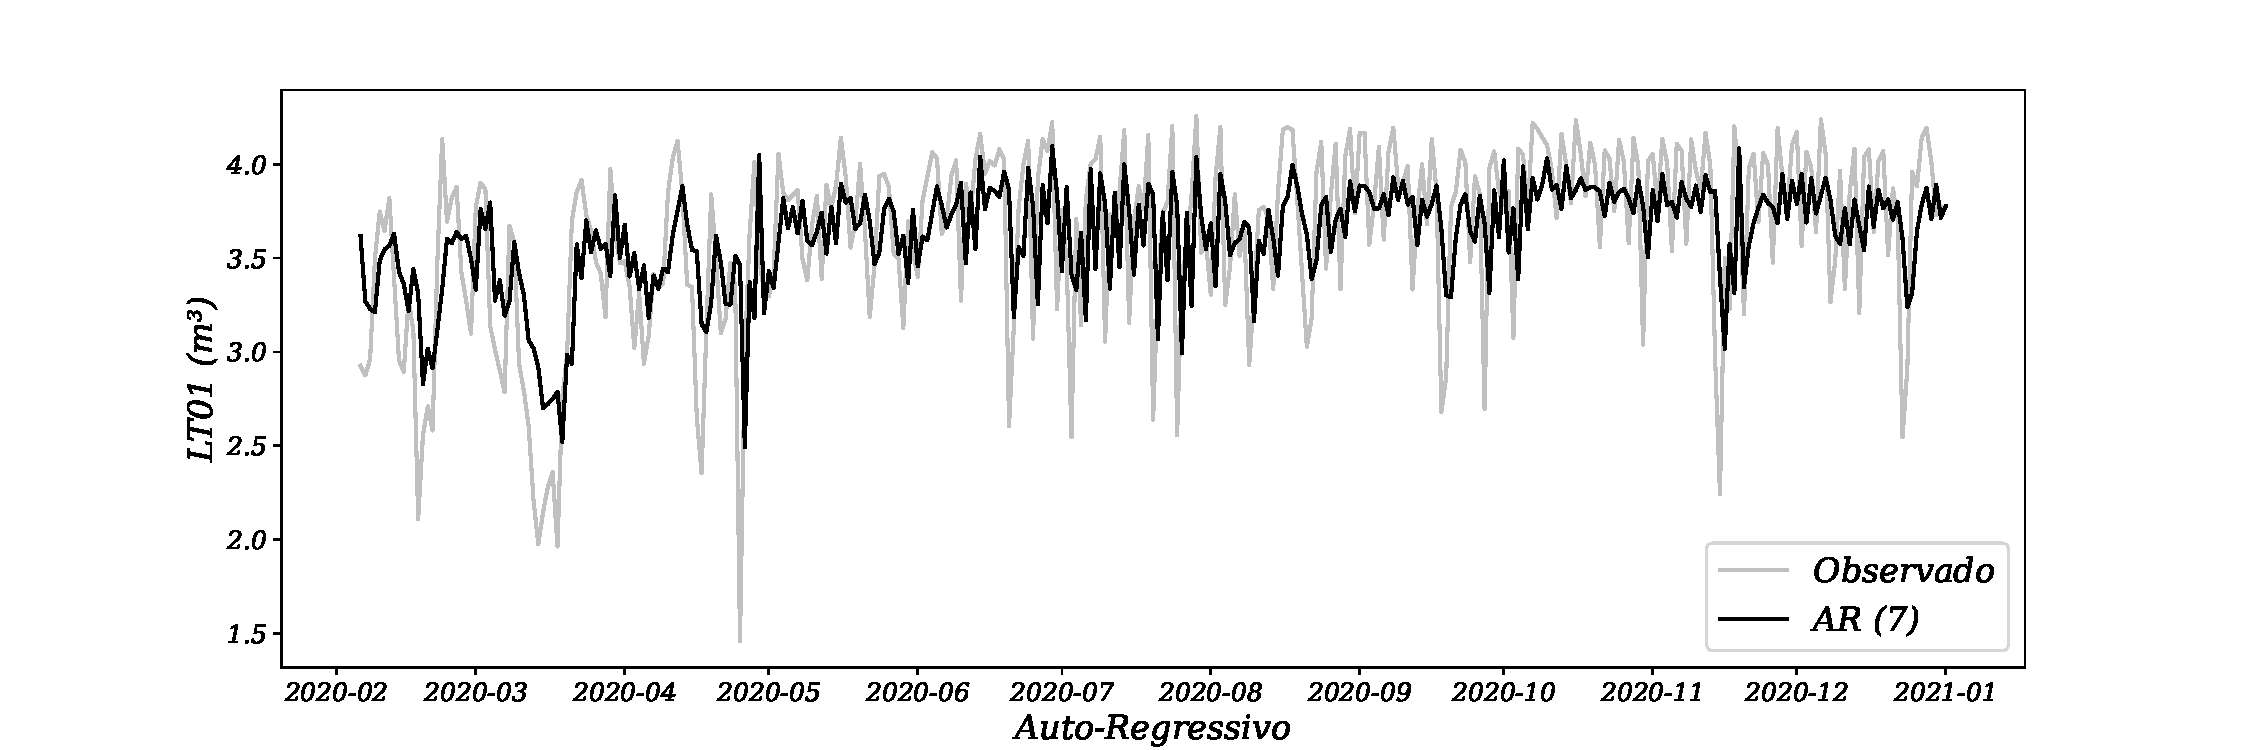
\includegraphics[width=\linewidth]{Modelos/Figuras/AR}
		\caption{Modelo AR(7)}
		\label{fig:1-ar}	
	\end{subfigure}
	
	\begin{subfigure}{1\textwidth}
		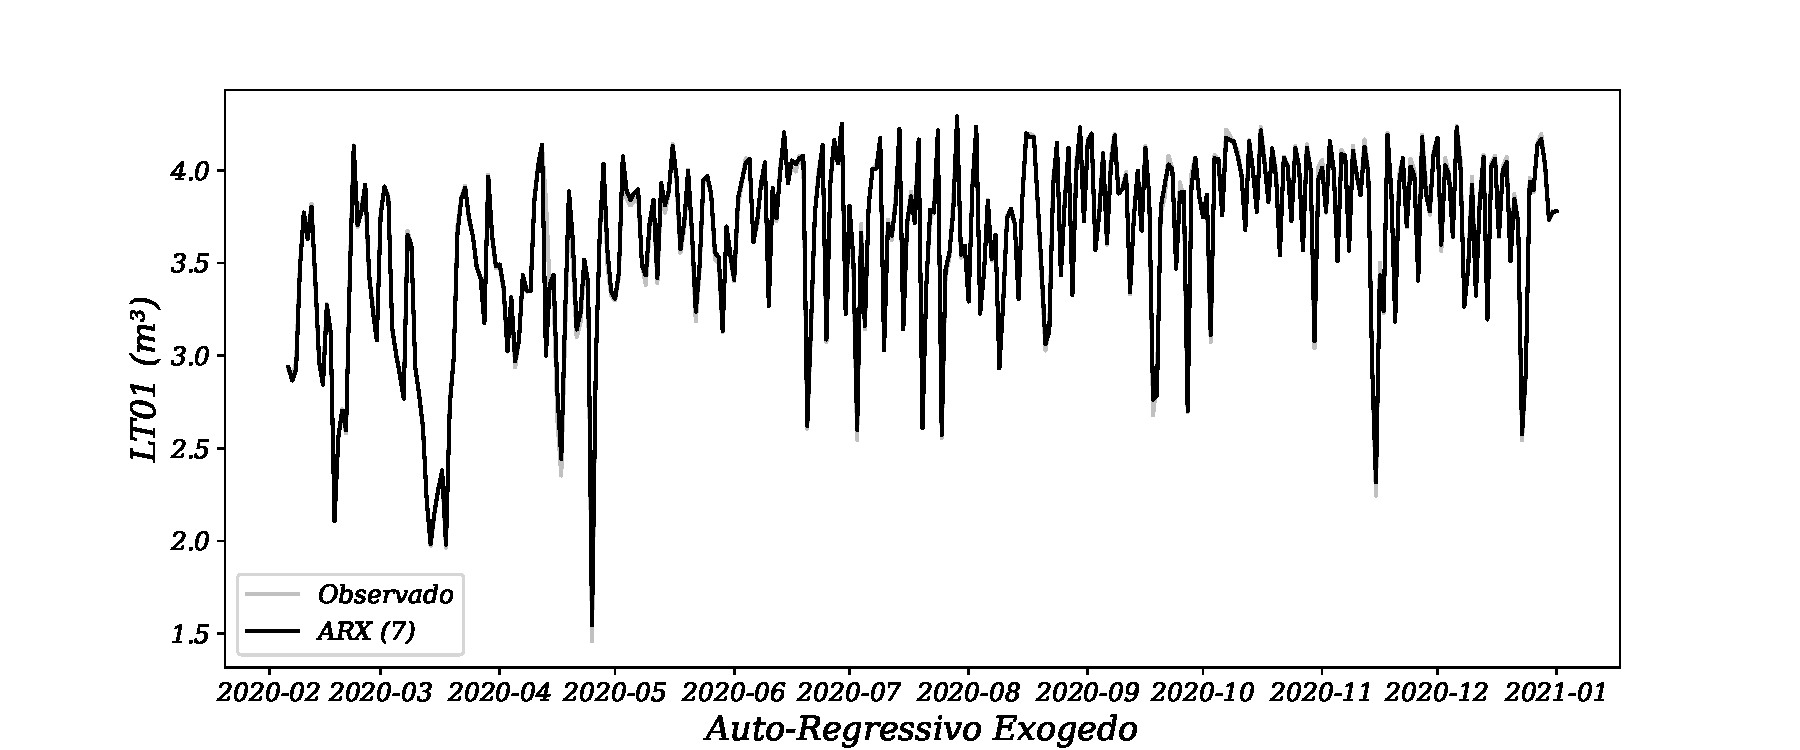
\includegraphics[width=\linewidth]{Modelos/Figuras/ARX}
		\caption{ARX (7)}
		\label{fig:1-arx}	
	\end{subfigure}
	
	\fonte{Elaboração própria a partir de dados da SANEPAR (2018 a 2020)}
\end{figure}



Na equação \eqref{AR}, o termo $\varepsilon_t$ representa o ruído branco. Essa equação pode ser entendida como uma regressão múltipla, em que os valores defasados de $y_t$ são utilizados como preditores. Esse modelo é conhecido como modelo autorregressivo de ordem $p$, ou AR(p).

A Figura \ref{fig:1-ar} tem como objetivo apresentar uma previsão de um passo à frente (um dia). Nos apêndices \ref{sec:ararxma24}, pode-se observar uma comparação entre os modelos AR, MA e ARX.

O modelo ARX é uma extensão do modelo AR, que incorpora variáveis exógenas nos dados para melhorar as previsões futuras. Esse modelo também é multivariado, como mostrado na subseção \ref{subsec:mult}, e foi incluído aqui para fins de comparação com o modelo AR simples, considerando a presença de variáveis exógenas.

Embora o modelo AR possa ser visualmente adequado para a previsão que está sendo feita, é importante destacar que, por ser um modelo autorregressivo, ele realiza previsões lineares e não captura padrões não lineares presentes nos dados. Para uma análise mais abrangente da série temporal, é necessário considerar exemplos de casos gerais.

\subsubsection{AR(0): Ru\'ido branco}

Se o parâmetro $p$ for definido como zero (AR($0$)), significa que não há termos autorregressivos no modelo. Nesse caso, a série temporal se comporta como um ruído branco. Cada ponto de dados é amostrado de uma distribuição com média zero e variância igual a sigma-quadrado. Isso resulta em uma sequência de números aleatórios que não exibem nenhum padrão ou correlação.

Essa propriedade do ruído branco pode ser útil em análises estatísticas, pois serve como uma hipótese nula. Ao comparar diferentes modelos ou testar a presença de padrões em uma série temporal, podemos usar o ruído branco como referência para avaliar se os resultados observados são estatisticamente significativos ou apenas resultado do acaso. Isso nos ajuda a evitar a detecção de padrões falsos positivos e garante a confiabilidade das análises realizadas.

\subsubsection{AR(1): Caminhadas aleat\'orias e Oscila\c c\~oes}

Com o parâmetro $p$ definido como $1$, o modelo AR leva em consideração o valor anterior da série temporal multiplicado por um coeficiente e, em seguida, adiciona ruído branco. Quando o coeficiente é igual a $0$, temos apenas ruído branco, resultando em uma série de tempo completamente aleatória, sem padrões previsíveis.

Quando o coeficiente é igual a $1$, temos uma caminhada aleatória, onde cada valor da série é obtido somando-se o valor anterior a um termo de ruído branco. Nesse caso, os valores da série apresentam uma tendência linear, aumentando ou diminuindo ao longo do tempo sem retornar à média.

Se o coeficiente estiver na faixa $0 < \alpha < 1$, temos o fenômeno de reversão média. Isso significa que os valores da série tendem a oscilar em torno de uma média central e a regressar em direção a ela após se afastarem. Esse padrão indica uma tendência de retorno à média ao longo do tempo.

Os diferentes comportamentos da série temporal, determinados pelo coeficiente no modelo AR, têm implicações importantes na análise e previsão de dados. A compreensão desses padrões é fundamental para escolher o modelo adequado e interpretar corretamente os resultados obtidos.

\subsubsection{AR(p): Termos de ordem superior}

Aumentar ainda mais o parâmetro $p$ no modelo AR significa considerar um número crescente de medições de tempo anteriores, cada uma multiplicada pelo seu próprio coeficiente. Isso permite levar em conta uma memória mais longa da série temporal e capturar padrões de dependência mais complexos ao longo do tempo.

No entanto, é importante ter em mente que aumentar excessivamente o valor de $p$ pode levar a problemas de \textit{overfitting}, onde o modelo se ajusta muito bem aos dados de treinamento, mas tem um desempenho ruim na previsão de novos dados. Portanto, é necessário encontrar um equilíbrio entre a complexidade do modelo e sua capacidade de generalização.

Além disso, é comum combinar o modelo AR com o modelo de média móvel (MA) para formar o modelo ARMA. O modelo MA considera os erros passados, ou seja, as diferenças entre os valores reais e as previsões anteriores, ajustadas por coeficientes. A combinação dos componentes AR e MA permite capturar tanto a dependência autorregressiva quanto a dependência na média móvel, proporcionando uma modelagem mais abrangente da série temporal.

Em suma, aumentar o parâmetro $p$ no modelo AR pode melhorar a capacidade do modelo de capturar padrões complexos da série temporal, mas é necessário ter cuidado para evitar \textit{overfitting}. A combinação com o modelo MA pode fornecer uma modelagem mais completa dos dados. A escolha adequada dos parâmetros depende da análise cuidadosa dos padrões presentes na série temporal e do equilíbrio entre a complexidade do modelo e sua capacidade de generalização.

\subsubsection{M\'edia M\'ovel}\label{subsubsec:ma}
No modelo de média móvel (MA), o componente não é uma média móvel simples, mas sim uma combinação de termos de erro de previsão defasados. O parâmetro $q$ no modelo MA representa o número de termos de erro de previsão que são levados em consideração na previsão.

De acordo com \citeonline{signal} este componente não é uma média de rolamento, mas sim os atrasos no ruído branco.

Em um modelo MA(1), por exemplo, a previsão é composta por um termo constante, o produto do termo de erro de previsão anterior por um multiplicador, e o termo de erro de previsão atual. Essa abordagem baseia-se em princípios estatísticos e de probabilidade, ajustando a previsão com base em termos anteriores de erro de previsão.

O modelo MA é uma alternativa ao modelo AR e é usado para capturar padrões de dependência na média móvel, ou seja, a influência de erros passados na previsão atual. Ao combinar o modelo AR e o modelo MA, como no modelo ARMA, é possível obter uma modelagem mais abrangente que considera tanto a dependência autorregressiva quanto a dependência na média móvel.

Portanto, o modelo MA leva em conta os termos de erro de previsão defasados para ajustar a previsão atual, permitindo considerar a probabilidade e estatística na modelagem da série temporal.


\begin{eqnarray}
	y_t=c+\varepsilon_t+\theta_1 \varepsilon_{t-1}+\theta_2 \varepsilon_{t-2}+\cdots+\theta_q \varepsilon_{t-q}\label{eq:ma}
\end{eqnarray}

Na equação \eqref{eq:ma}, em que $\varepsilon_t$ representa o ruído branco, esse modelo é conhecido como um modelo de média móvel $MA(q)$, em que $q$ é a ordem da média móvel. É importante ressaltar que não observamos diretamente os valores de $\varepsilon_t$, portanto, essa modelagem não se trata de uma regressão no sentido convencional.

Diferentemente de uma regressão comum em que temos variáveis explicativas observadas, no modelo $MA(q)$, estamos usando os termos de ruído branco defasados para estimar e prever os valores da série temporal. O objetivo é capturar a dependência dos termos de erro passados na previsão atual.

Esse modelo é útil para modelar séries temporais em que a média móvel tem um impacto significativo nas observações. Ao ajustar a série temporal com base nos termos de ruído branco defasados, podemos obter uma estimativa mais precisa dos valores futuros.

Embora o modelo $MA(q)$ seja diferente de uma regressão tradicional, ele é uma ferramenta estatística poderosa para modelar e prever séries temporais, levando em consideração a dependência entre os termos de erro passados.

\begin{figure}[!htb]
	\centering
	\caption{Modelo MA(7) }
	\label{fig:1-ma}
	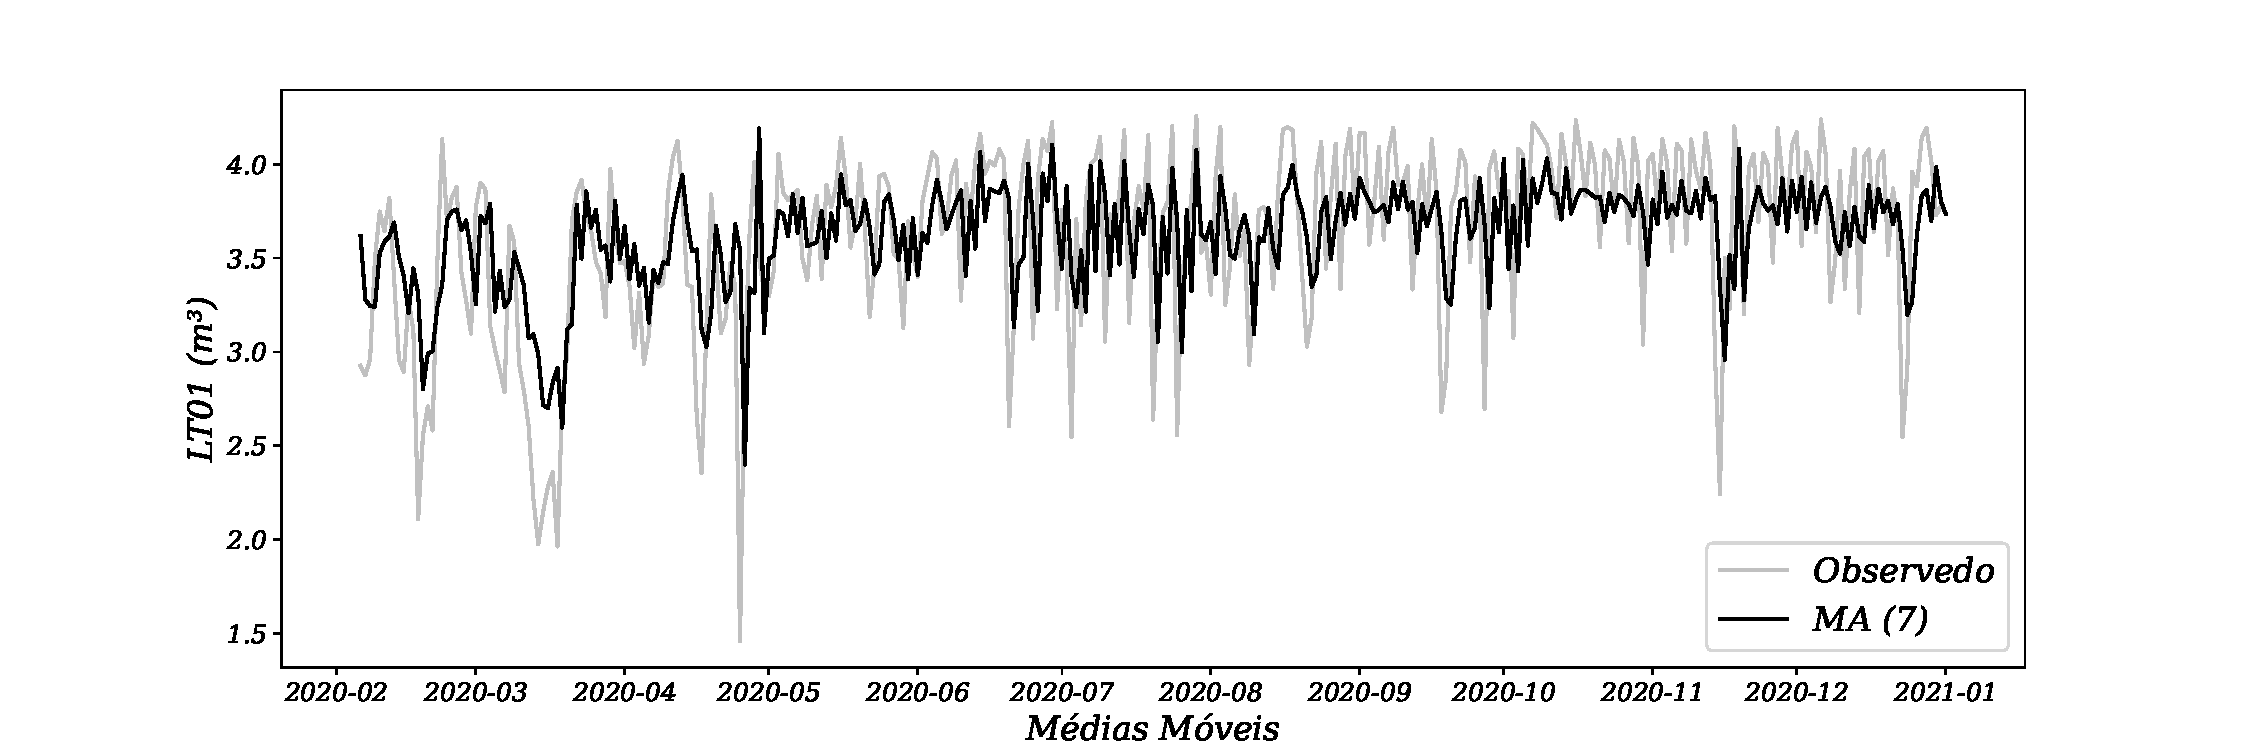
\includegraphics[width=1\linewidth]{Modelos/Figuras/MA}
	
	\fonte{Elaboração própria a partir de dados da SANEPAR (2018 a 2020)}
\end{figure}

O modelo MA, quando comparado com o modelo AR de mesma ordem, facilita a previsão. Conforme ilustrado na Figura \ref{fig:1-ma}, a previsão gráfica se assemelha ao modelo apresentado na Figura \ref{fig:1-ar}, embora não seja comparável ao modelo exibido na Figura \ref{fig:1-arx}. É importante notar que esse modelo aparenta prever com precisão o período de tempo que foi considerado.

\subsubsection{Modelos ARMA e ARIMA}\label{subsubsec:arma}
A arquitetura ARMA é uma combinação dos modelos AR  e MA, onde o modelo AR é adicionado ao modelo MA.

No modelo ARMA, é adicionada uma constante à soma dos termos autorregressivos multiplicados pelos seus coeficientes, juntamente com a soma dos termos de média móvel multiplicados pelos seus coeficientes, além do ruído branco. Essa estrutura é amplamente utilizada em diversos modelos de previsão em diferentes áreas.

\begin{figure}[!htb]
	\centering
	\caption{ARMA (7,7)}
	\label{fig:1-arma}
	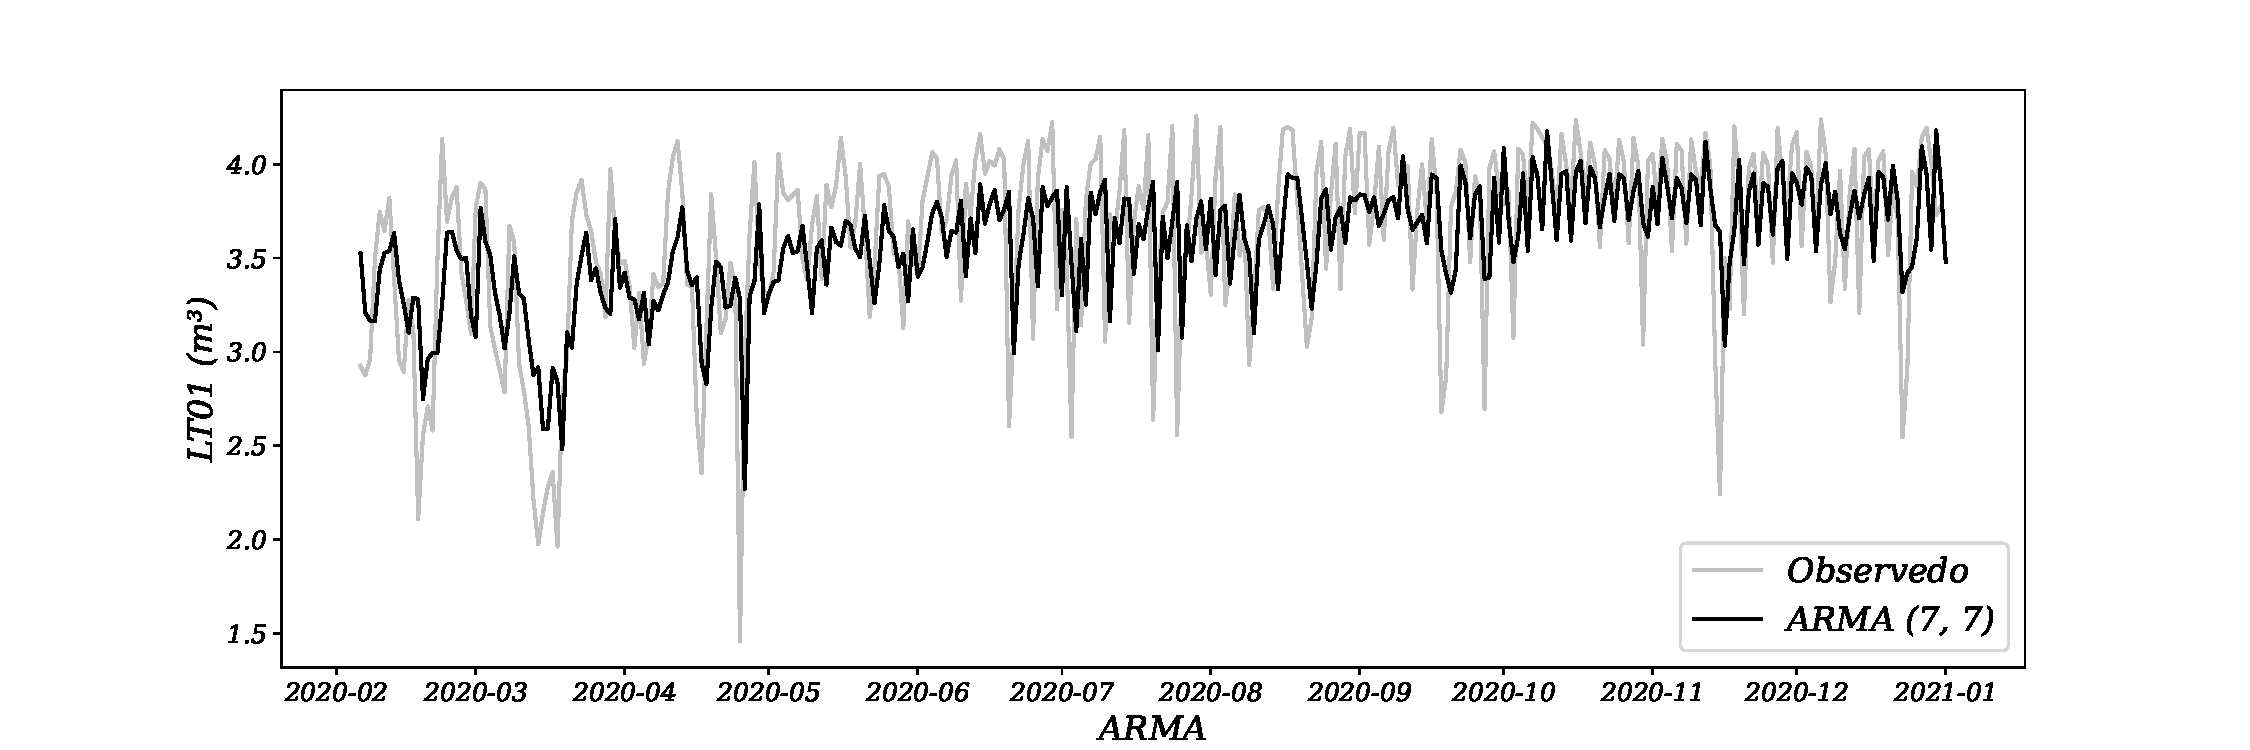
\includegraphics[width=1\linewidth]{Modelos/Figuras/ARMA}
	
	\fonte{Elaboração própria a partir de dados da SANEPAR (2018 a 2020)}
\end{figure}

A Figura \ref{fig:1-arma} ilustra a combinação dos modelos AR e MA em um modelo ARMA. Essa abordagem pode levar a uma redução significativa no erro de previsão, como observado nos apêndices \ref{sec:comtb24} e \ref{sec:comtb18}, onde são apresentadas comparações com um maior número de passos de previsão.

\subsubsection{ARIMA}

\begin{eqnarray}
	Y_t = \beta_2 + \omega_1\varepsilon_{t-1} + \omega_2 \varepsilon_{t-2} +\ldots+ \omega_q \varepsilon_{t-q} + \varepsilon_t \label{arima}
\end{eqnarray}

Na equação \eqref{arima}, a variável $Y_t$ representa a série temporal que foi diferenciada (possivelmente mais de uma vez). Os ``preditores'' no lado direito da equação incluem os valores defasados de $Y_t$ e os erros defasados. Esse tipo de modelo é conhecido como ARIMA ($p, d, q$).

O modelo ARIMA é uma extensão do modelo ARMA que incorpora uma etapa adicional de pré-processamento chamada de diferenciação. Essa etapa é representada pela notação \textbf{I(d)}, em que \textbf{d} denota a ordem de diferenciação, ou seja, o número de transformações necessárias para tornar a série temporal estacionária. Portanto, um modelo ARIMA é simplesmente um modelo ARMA aplicado à série temporal diferenciada. Isso permite lidar com séries temporais que possuem tendências ou padrões não estacionários.

\begin{figure}[!htb]
	\centering
	\caption{ARIMA (7,1,7)}
	\label{fig:1-arima}
	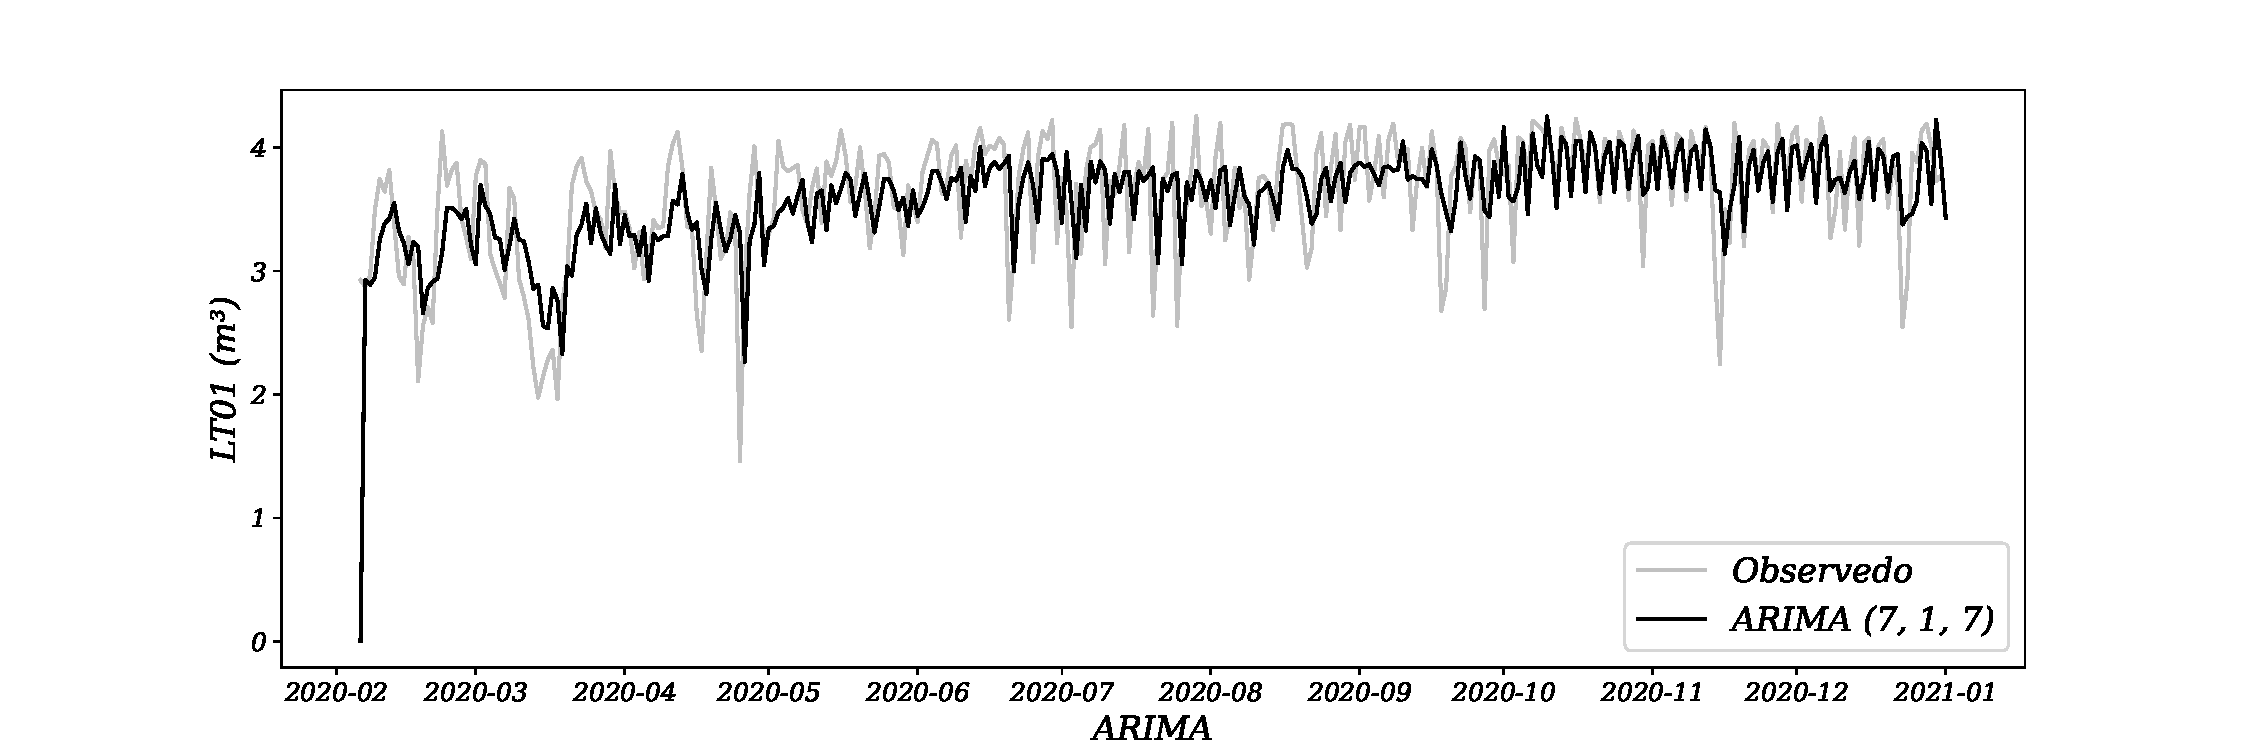
\includegraphics[width=1\linewidth]{Modelos/Figuras/ARIMA}
	
	Fonte: Elaboração própria a partir de dados da SANEPAR (2018 a 2020)
\end{figure}

Ao analisar a Figura \ref{fig:1-arima}, não se nota uma diferença visual significativa em relação aos outros métodos apresentados anteriormente. O método ARX ainda parece ser superior aos demais com base na análise visual.

Embora os modelos ARIMA sejam eficazes, incorporar variáveis sazonais e exógenas ao modelo pode potencializar sua capacidade de previsão. No entanto, é importante destacar que o modelo ARIMA pressupõe que a série temporal seja estacionária. Quando lidamos com séries temporais não estacionárias, é necessário recorrer a outros modelos para a análise e previsão adequadas.

\subsubsection{SARIMA}

\begin{eqnarray}
	Y_t&=&c+\sum_{n=1}^p \alpha_n y_{t-n}+\sum_{n=1}^q \theta_n \epsilon_{t-n}+\sum_{n=1}^P \phi_n y_{t-s n}+\sum_{n=1}^Q \eta_n \epsilon_{t-s n}+\epsilon_t \label{sarima}
\end{eqnarray}

O modelo proposto é uma extensão do modelo ARIMA, com a adição de componentes autorregressivos e de média móvel sazonal. Esses componentes extras são ajustados levando em consideração os padrões sazonais presentes nos dados, utilizando atrasos correspondentes à frequência sazonal (por exemplo, 12 para dados mensais). Essa abordagem permite capturar e modelar de forma mais precisa as variações sazonais e melhorar a qualidade das previsões em séries temporais com esse comportamento cíclico.

\begin{figure}[!htb]
	\centering
	\caption{SARIMA $(7,1,7) (2,1,1)_{12}$}
	\label{fig:1-sarima}
	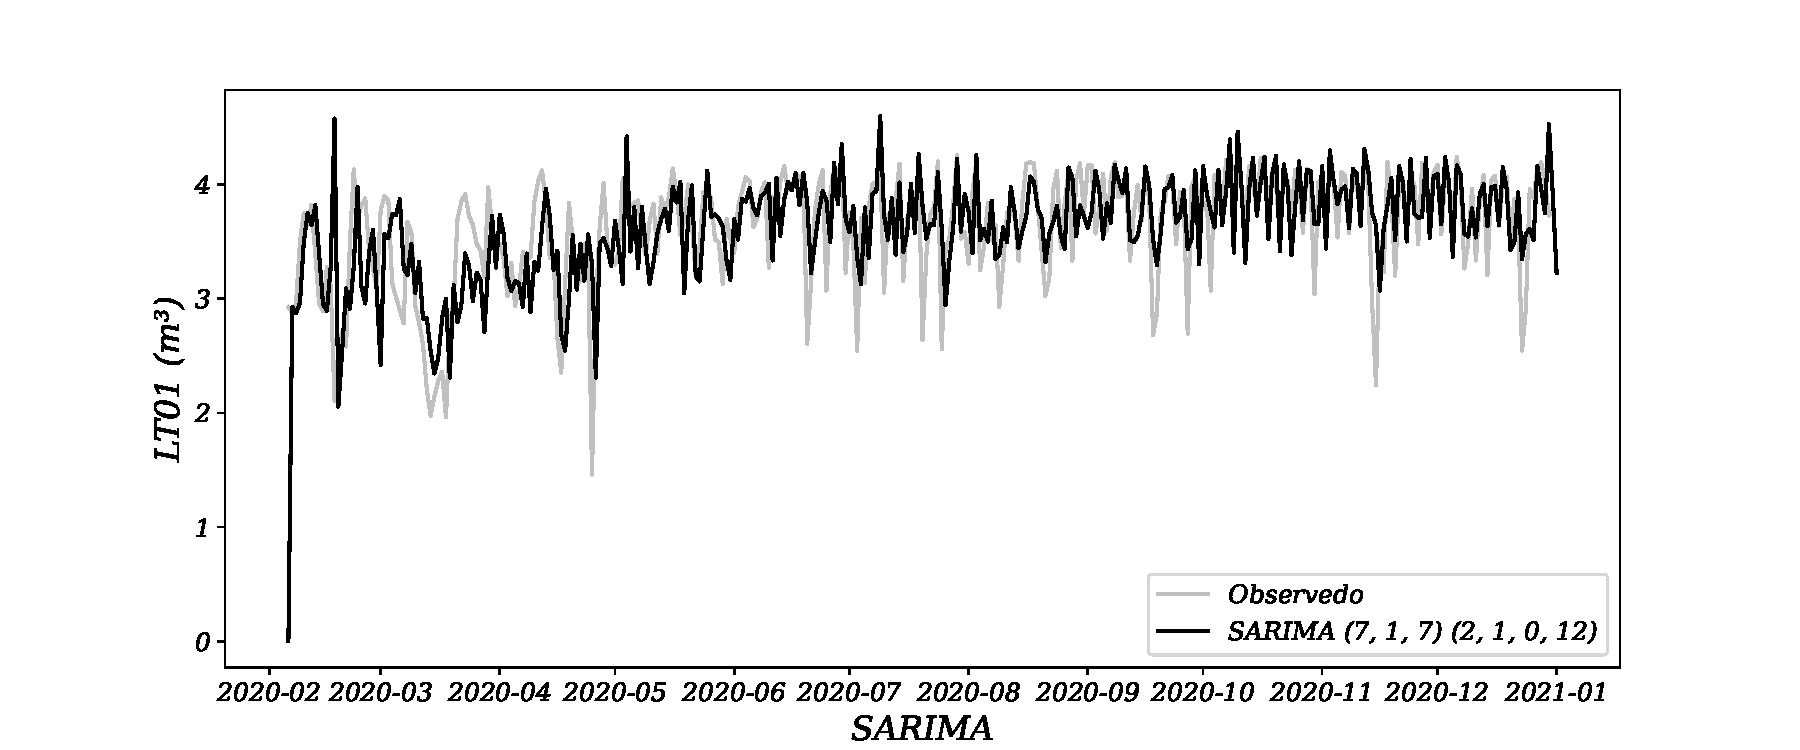
\includegraphics[width=1\linewidth]{Modelos/Figuras/SARIMA}
	
	\fonte{Elaboração própria a partir de dados da SANEPAR (2018 a 2020)}
\end{figure}

Na Figura \ref{fig:1-sarima}, é possível observar que a previsão em vermelho está mais próxima dos valores observados em preto, mostrando que a inclusão do componente de sazonalidade melhora a qualidade da previsão. Os modelos SARIMA são capazes de lidar com dados que apresentam padrões sazonais, permitindo a diferenciação dos dados em termos de componentes sazonais e não sazonais. Uma abordagem útil para determinar os melhores parâmetros do modelo é utilizar uma estrutura de pesquisa automatizada de parâmetros, como o pmdarima, que auxilia na identificação dos parâmetros ideais para o modelo SARIMA. Isso pode contribuir para uma melhor compreensão e ajuste do modelo aos dados observados.

\subsection{Modelos de S\'erie Temporal Multivariada}\label{subsec:mult}

Os Modelos de Série Temporal Multivariada são uma abordagem estatística utilizada para analisar e prever dados que possuem múltiplas variáveis dependentes ao longo do tempo. Nesse tipo de modelo, considera-se a interdependência entre as diferentes séries temporais, permitindo a análise conjunta e a identificação de padrões e relações entre as variáveis. Esses modelos são aplicados em diversas áreas, como economia, finanças, meteorologia e análise de dados, proporcionando insights valiosos para a compreensão e previsão de fenômenos complexos ao longo do tempo.

\subsubsection{ARIMAX e SARIMAX}

\begin{eqnarray}
	d_t=c+\sum_{n=1}^p \alpha_n d_{t-n}+\sum_{n=1}^q \theta_n \epsilon_{t-n}+\sum_{n=1}^r \beta_n x_{n_t}+\sum_{n=1}^P \phi_n d_{t-s n}+\sum_{n=1}^Q \eta_n \epsilon_{t-s n}+\epsilon_t \label{eq:sarmax}
\end{eqnarray}

Em \eqref{eq:sarmax}, o modelo SARIMAX é apresentado. Nesse modelo, são consideradas variáveis exógenas, ou seja, são utilizados dados externos para a realização das previsões. É importante ressaltar que mesmo que essas variáveis exógenas sejam indiretamente modeladas no histórico de previsões do modelo, ao incluí-las diretamente, o modelo será capaz de responder de forma mais ágil aos efeitos dessas variáveis. Isso significa que a incorporação de informações externas possibilita uma resposta mais rápida e precisa do modelo em relação aos fatores externos, resultando em previsões mais atualizadas e acuradas.

\begin{figure}[!htb]
	\centering
	\caption{Comparação entre ARIMAX e SARIMAX}
	\begin{subfigure}{1\textwidth}
		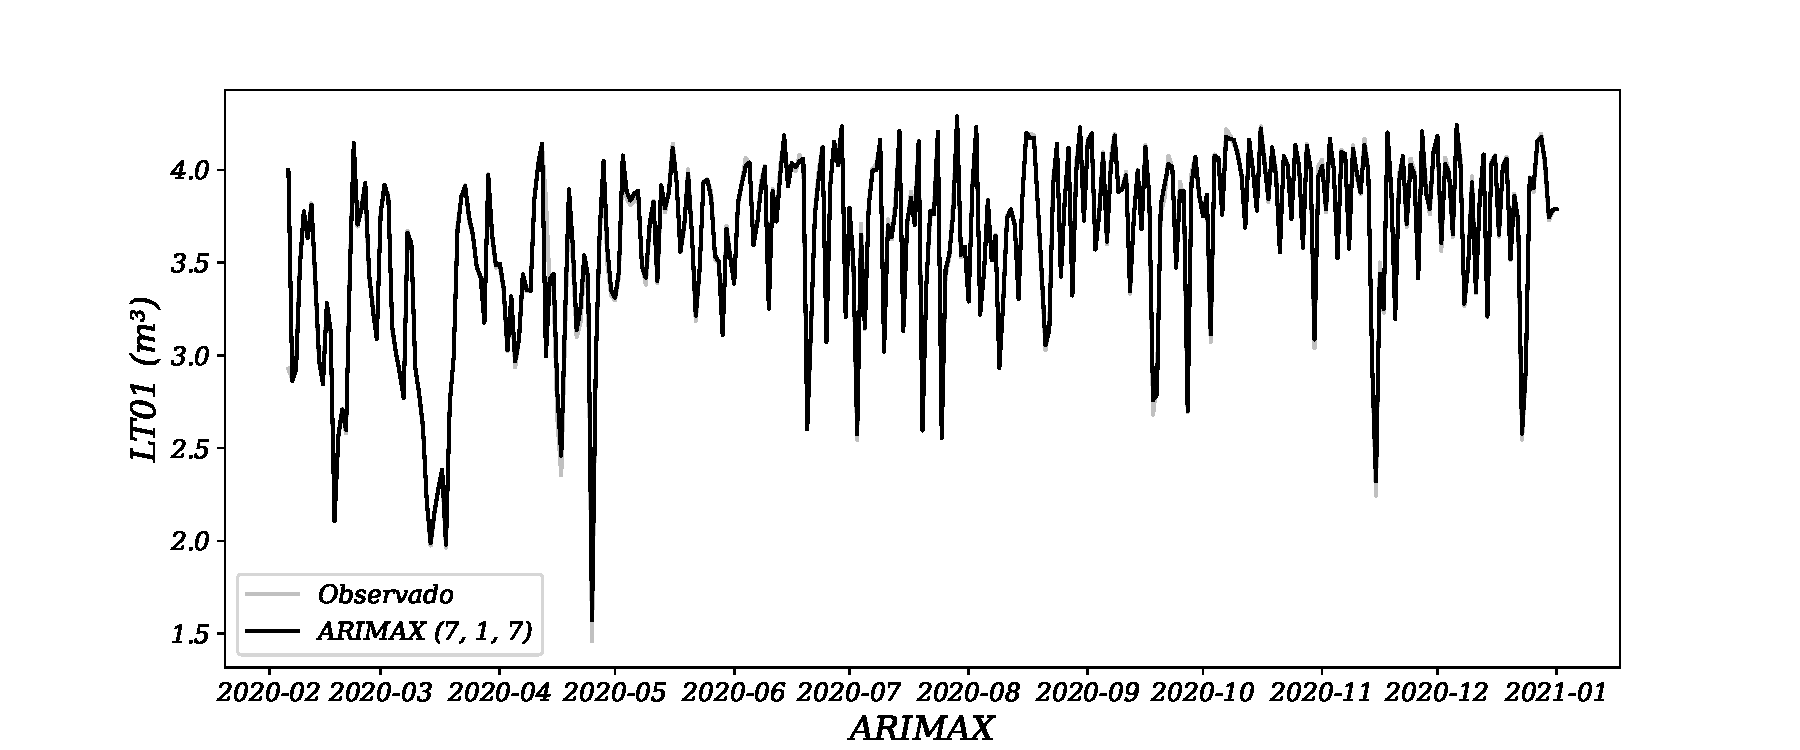
\includegraphics[width=\linewidth]{Modelos/Figuras/ARIMAX}
		\caption{ARIMAX $(7,1,7)$}
		\label{fig:1-arimax}
	\end{subfigure}
	\hfill
	
	\begin{subfigure}{1\textwidth}
		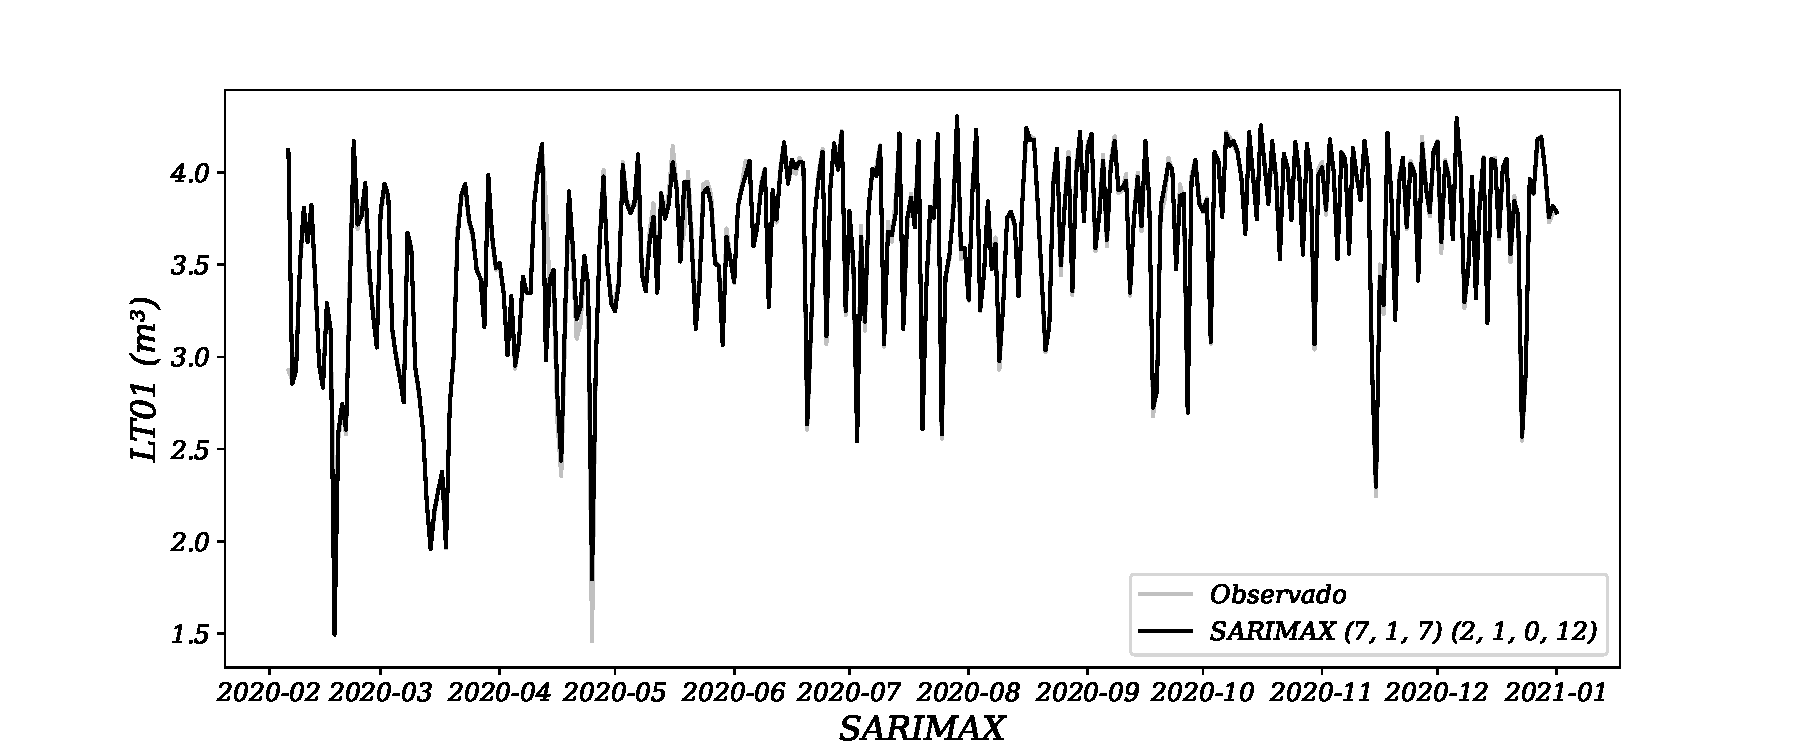
\includegraphics[width=\linewidth]{Modelos/Figuras/SARIMAX}
		\caption{SARIMAX $(7,1,7) (2,1,1)_{12}$}
		\label{fig:1-sarimax}	
	\end{subfigure}

		
	\fonte{Elaboração própria a partir de dados da SANEPAR (2018 a 2020)}
\end{figure}


Entre os modelos com variáveis exógenas, como mostrado nas Figuras \ref{fig:1-arimax} e \ref{fig:1-sarimax}, observa-se uma melhora significativa na qualidade das previsões em comparação com os modelos que não incluem variáveis exógenas. A adição dessas variáveis externas permite capturar melhor as influências e os padrões presentes nos dados, resultando em previsões mais completas e precisas. Essa inclusão de informações adicionais contribui para uma compreensão mais abrangente do comportamento da série temporal e possibilita uma melhor adaptação do modelo aos padrões observados.


\subsection{Modelos de Aprendizado de M\'aquina Supervisionados}\label{subsec:reg}

Os modelos regressivos para séries temporais têm sido amplamente reconhecidos e utilizados na literatura atual, especialmente aqueles baseados em métodos de gradiente. Esses modelos, incluindo a regressão linear simples, têm se destacado como uma escolha popular em competições de séries temporais em todo o mundo.

Esses modelos são valorizados por sua capacidade de capturar relações complexas e não lineares nos dados, permitindo previsões mais precisas e eficientes. Sua popularidade reflete o reconhecimento da eficácia desses modelos em abordar uma ampla gama de problemas de previsão de séries temporais em diferentes áreas de estudo.

A abordagem regressiva, combinada com técnicas de otimização baseadas em gradiente, tem se mostrado particularmente eficaz na obtenção de resultados de alta qualidade. Esses modelos são capazes de aprender a partir dos dados históricos e ajustar seus parâmetros de forma iterativa, otimizando assim o desempenho da previsão.

Com a crescente disponibilidade de dados e avanços na área de aprendizado de máquina, espera-se que os modelos regressivos para séries temporais continuem a evoluir e desempenhar um papel importante na análise e previsão de dados temporais em diversas aplicações.

\subsubsection{Regress\~ao Linear (LR)}

De acordo com o estudo realizado por \citeonline{korstanje2021}, nos modelos de aprendizado de máquina supervisionados, é feita uma tentativa de identificar as relações existentes entre diferentes variáveis:


\begin{itemize}
	\item Variável de destino: a variável que você tenta prever
	\item Variáveis explicativas: Variáveis que ajudam você a prever o alvo variável
\end{itemize}

Para realizar previsões, é importante que se compreenda quais tipos de variáveis explicativas podem ser utilizadas. Neste exemplo, a variável \textbf{Pressão de Sucção (PT01SU)} será considerada como a variável $x$, enquanto a variável \textbf{Nível do Reservatório (Câmara 1) LT01} será considerada como a variável $y$, com base na análise de correlação de Pearson ilustrada na Figura \ref{fig:person}. O coeficiente de correlação indica a relação entre o eixo $x$ e $y$, como expresso pela seguinte fórmula.



A fórmula do coeficiente de correlação de Pearson é dada por:

\begin{equation}
	r=\frac{\sum\left(x_i-\bar{x}\right)\left(y_i-\bar{y}\right)}{\sqrt{\left(\sum\left(x_i-\bar{x}\right)^2\right)\left(\sum\left(y_i-\bar{y}\right)^2\right)}}
\end{equation}

Onde $x_i$ e $y_i$ representam os valores das variáveis $X$ e $Y$, respectivamente. $\bar{x}$ e $\bar{y}$ são as médias dos valores $x_i$ e $y_i$. O coeficiente de correlação de Pearson mede a força e a direção da relação linear entre as variáveis $X$ e $Y$. Valores próximos a 1 indicam uma correlação positiva forte, valores próximos a -1 indicam uma correlação negativa forte, e valores próximos a 0 indicam uma ausência de correlação entre as variáveis.

\begin{figure}[H]
	\centering
	\caption{Corelação de Pearson}
	\label{fig:person}
	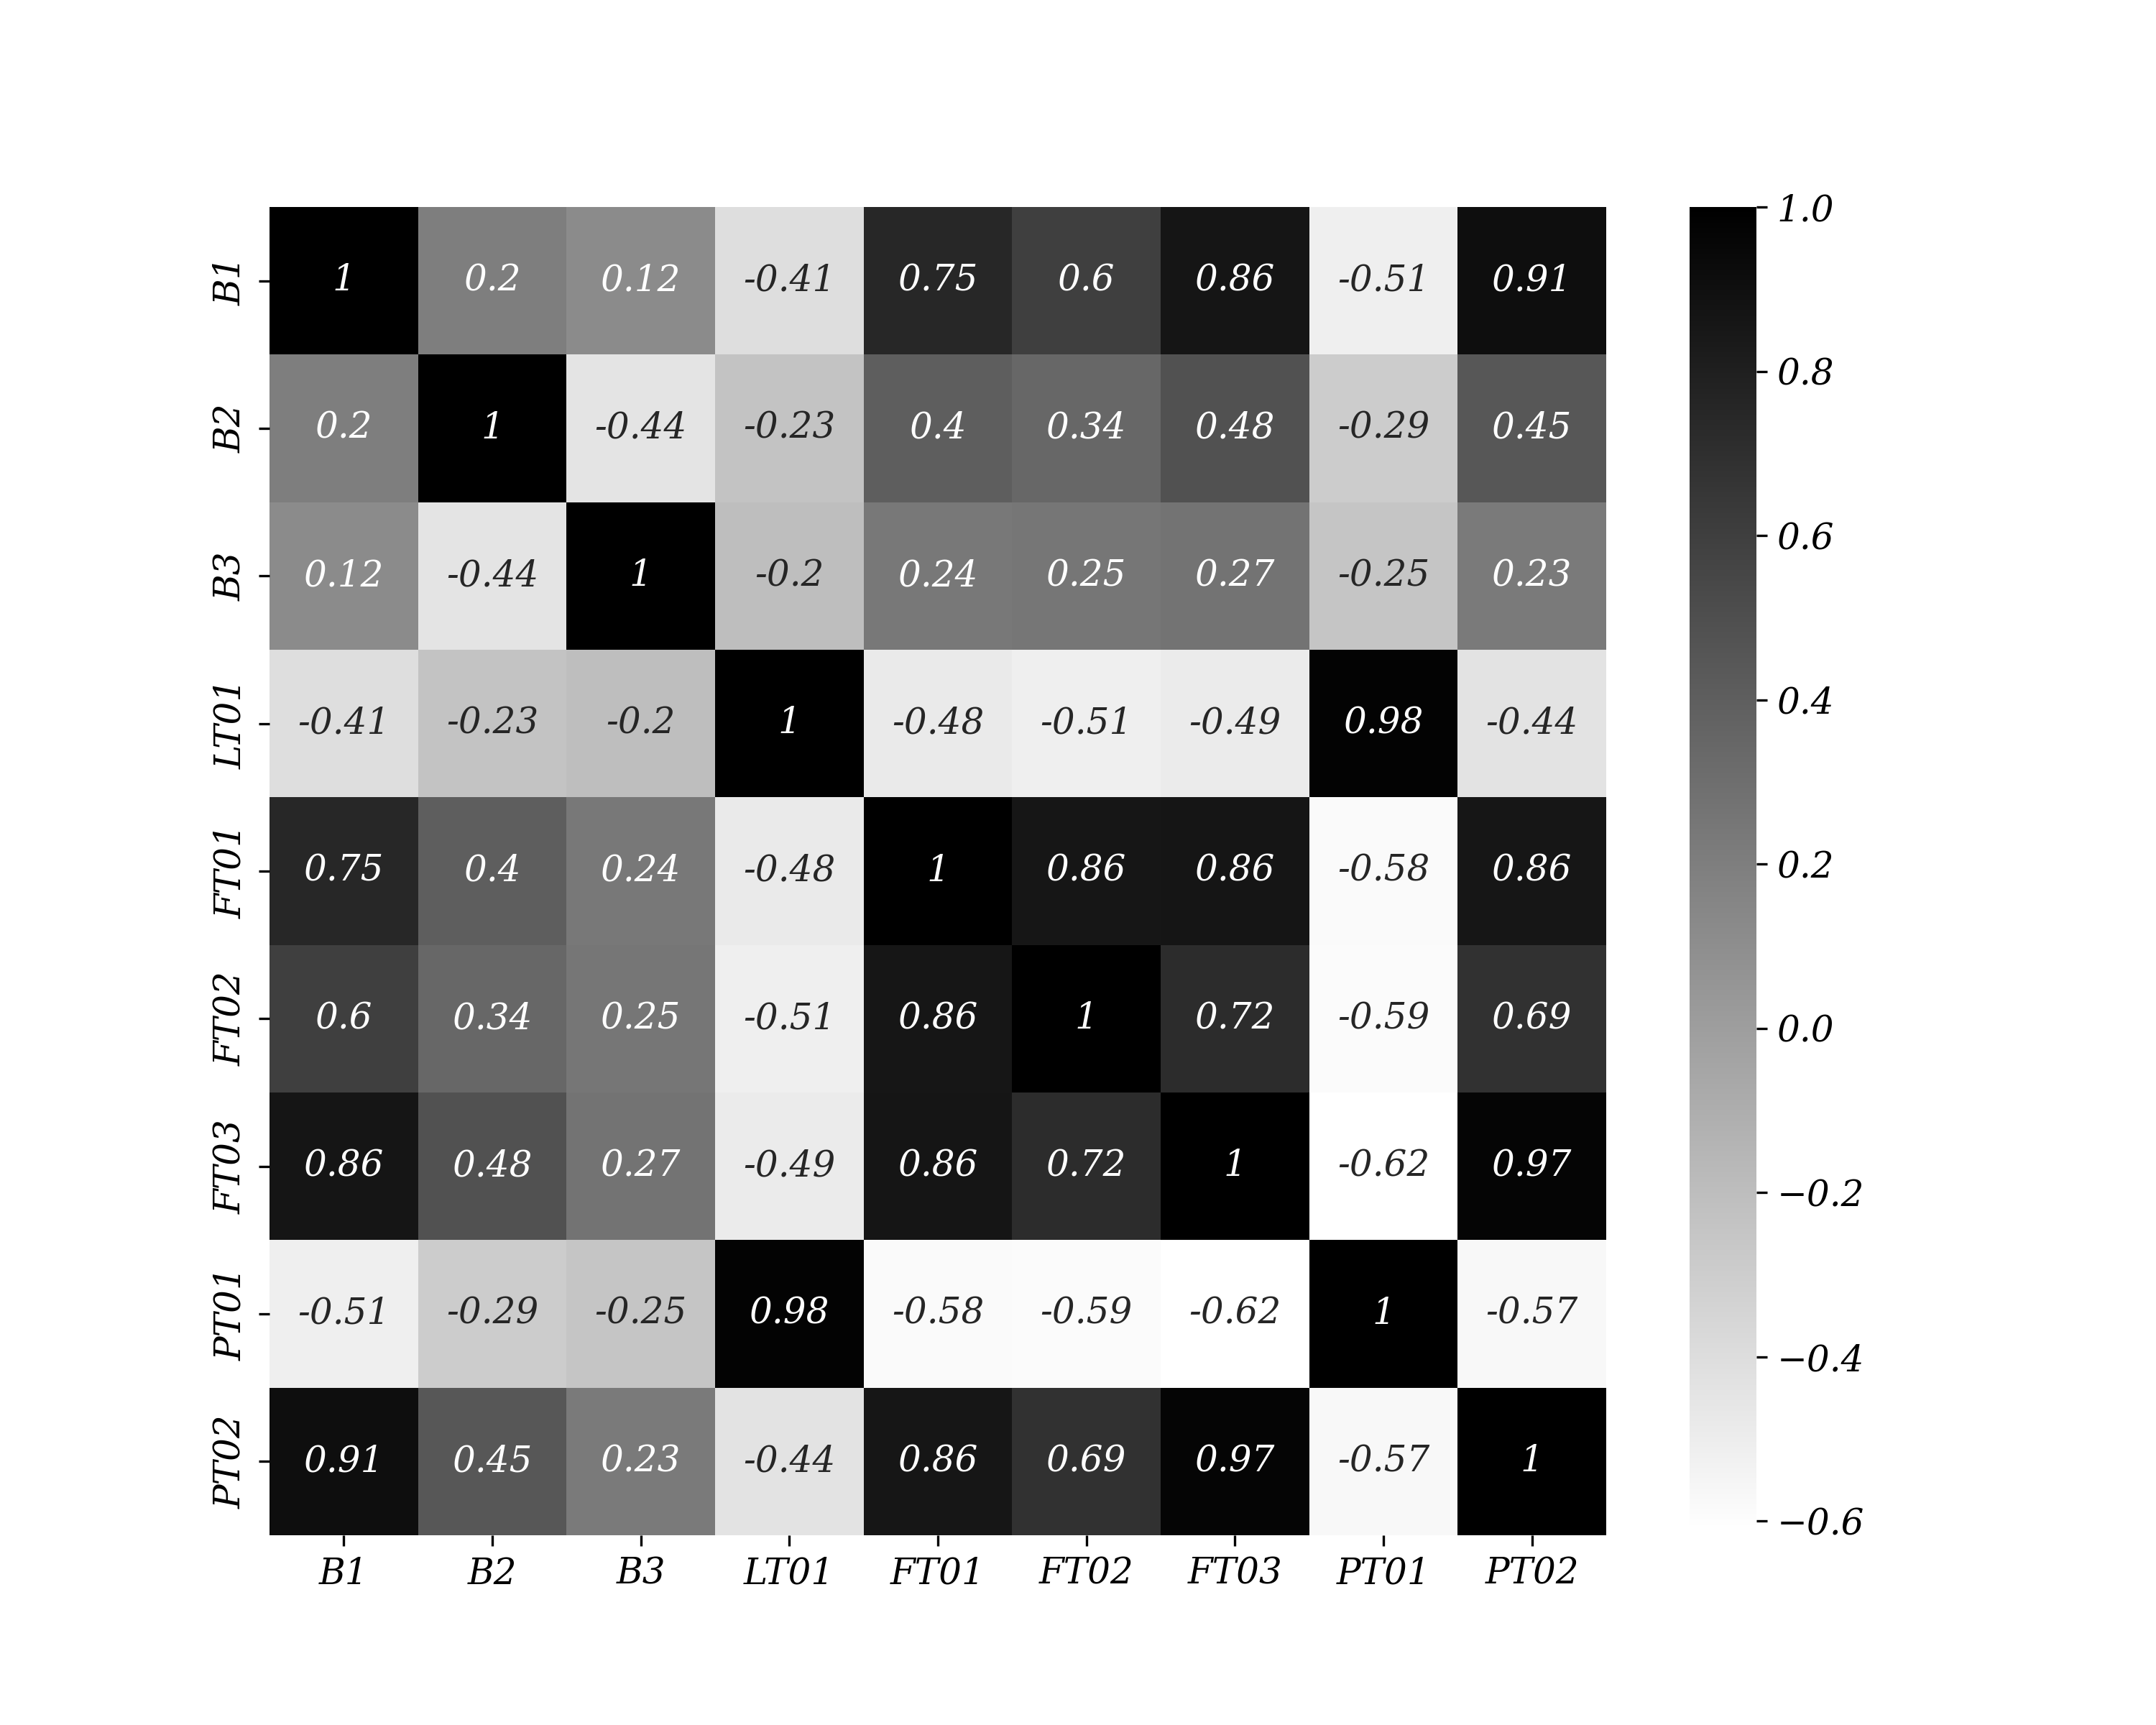
\includegraphics[width=0.9\linewidth]{Apendices/Figuras/modelagem-24h/person}
	
	Fonte: Elaboração própria a partir de dados da SANEPAR (2018 a 2020)
\end{figure}

A Figura \ref{fig:person} ilustra a correlação entre as variáveis no conjunto de dados em questão. Essa imagem representa graficamente a relação entre as variáveis e é usada para demonstrar a existência de uma correlação forte entre elas. Com base nessa análise, é possível responder à pergunta de pesquisa \ref{q1}, pois a correlação entre as variáveis é significativa.

\subsubsection{Defini\c c\~ ao do modelo}

A regressão linear é definida da seguinte forma:

\begin{equation}
	y = \beta_0 + \beta_1 x_1 + \cdots + \beta_p x_p + \varepsilon \label{eq:lr}
\end{equation}

Da Equação \eqref{eq:lr}, temos as seguintes variáveis:

\begin{itemize}
	\item Há $p$ variáveis explicativas, denotadas por $x$.
	\item Existe uma variável alvo, denotada por $y$.
	\item O valor de $y$ é calculado como uma constante $\beta_0$, somada aos valores das variáveis $x$ multiplicados por seus coeficientes $\beta_1$ a $\beta_p$.
\end{itemize}

\begin{figure}[H]
	\centering
	\caption{Regressão linear LT01 vs PT01 correlação 98\%}
	\label{fig:lr-lt01-m3}
	\includegraphics[width=0.9\linewidth]{"Modelos/Figuras/LR LT01 (m³)"}
	
	Fonte: Elaboração própria a partir de dados da SANEPAR (2018 a 2020)
\end{figure}



A Figura \ref{fig:lr-lt01-m3} fornece uma representação visual da interpretação dos coeficientes $\beta_0$ e $\beta_1$. Ela ilustra que um aumento de $1$ na variável $x$ está associado a um aumento proporcional de $\beta_1$ na variável $y$. O valor de $\beta_0$ representa o valor de $y$ quando $x$ é igual a $0$.

Para utilizar a regressão linear, é necessário estimar os coeficientes (betas) com base em um conjunto de dados de treinamento. Esses coeficientes podem ser estimados por meio da seguinte fórmula, expressa em notação matricial:

\begin{eqnarray}
	\hat{\beta}&=&\left(X^T X\right)^{-1} X^T y\label{eq:ols}
\end{eqnarray}

A fórmula mencionada, conhecida como \textbf{OLS} (método dos mínimos quadrados ordinários), é amplamente utilizada na regressão linear \citeonline{korstanje2021}. Esse método é conhecido por ser rápido de ajustar, pois requer apenas cálculos matriciais para estimar os coeficientes $\beta$. No entanto, ele é mais adequado para processos lineares e pode ser menos adequado para modelos mais complexos que envolvam relações não-lineares. Portanto, é importante considerar suas limitações ao aplicar a regressão linear em contextos mais complexos.

\begin{figure}[H]
	\centering
	\caption{Regressão linear (LR) um passo a frente}
	\label{fig:1-regressao-linear}
	\includegraphics[width=0.9\linewidth]{Modelos/Figuras/0-regressão-linear}
	
	Fonte: Elaboração própria a partir de dados da SANEPAR (2018 a 2020)
\end{figure}


\subsubsection{Floresta Aleat\'oria (Random Forest)} \label{subsubsec:rf}

Pode-se observar que ter exatamente a mesma árvore de decisão repetidas vezes não adiciona valor significativo em comparação a usar essa mesma árvore de decisão apenas uma vez. Em modelos de conjunto, cada modelo individual deve ser ligeiramente diferente dos demais. Existem dois métodos amplamente reconhecidos para criar conjuntos: o ensacamento (\textit{bagging}) e o reforço (\textit{boosting}). A floresta aleatória utiliza o ensacamento para criar um conjunto de árvores de decisão, onde cada árvore é construída com uma amostra aleatória do conjunto de dados original. Isso garante que as árvores sejam distintas e diversificadas, contribuindo para a robustez e eficácia do modelo.


\begin{figure}[H]
	\centering
	\caption{Regressão da Floresta Aleatória (RFR)}
	\label{fig:1-regressao-rfa}
	\includegraphics[width=0.9\linewidth]{Modelos/Figuras/0-regressão-rfa}
	
	Fonte: Elaboração própria a partir de dados da SANEPAR (2018 a 2020)
\end{figure}


Segundo \citeonline{Pelletier2016156}, cada árvore em um modelo de Floresta Aleatória de Regressão (RFR) é construída por meio de um algoritmo de aprendizado individual que divide o conjunto de variáveis de entrada em subconjuntos, com base em um teste de valor de atributo, como o coeficiente de Gini. Ao contrário das árvores de decisão clássicas, as árvores de RFR são construídas sem poda e selecionam aleatoriamente um subconjunto de variáveis de entrada em cada nó. Atualmente, o número de variáveis utilizadas para dividir um nó em uma RFR (denotado por $m$) corresponde à raiz quadrada do número total de variáveis de entrada. Essa abordagem ajuda a aumentar a diversidade das árvores e aprimorar o desempenho do modelo.

\begin{figure}[H]
	\centering
	\caption{Esquema da Floresta Aleatória}
	\label{fig:rf}
	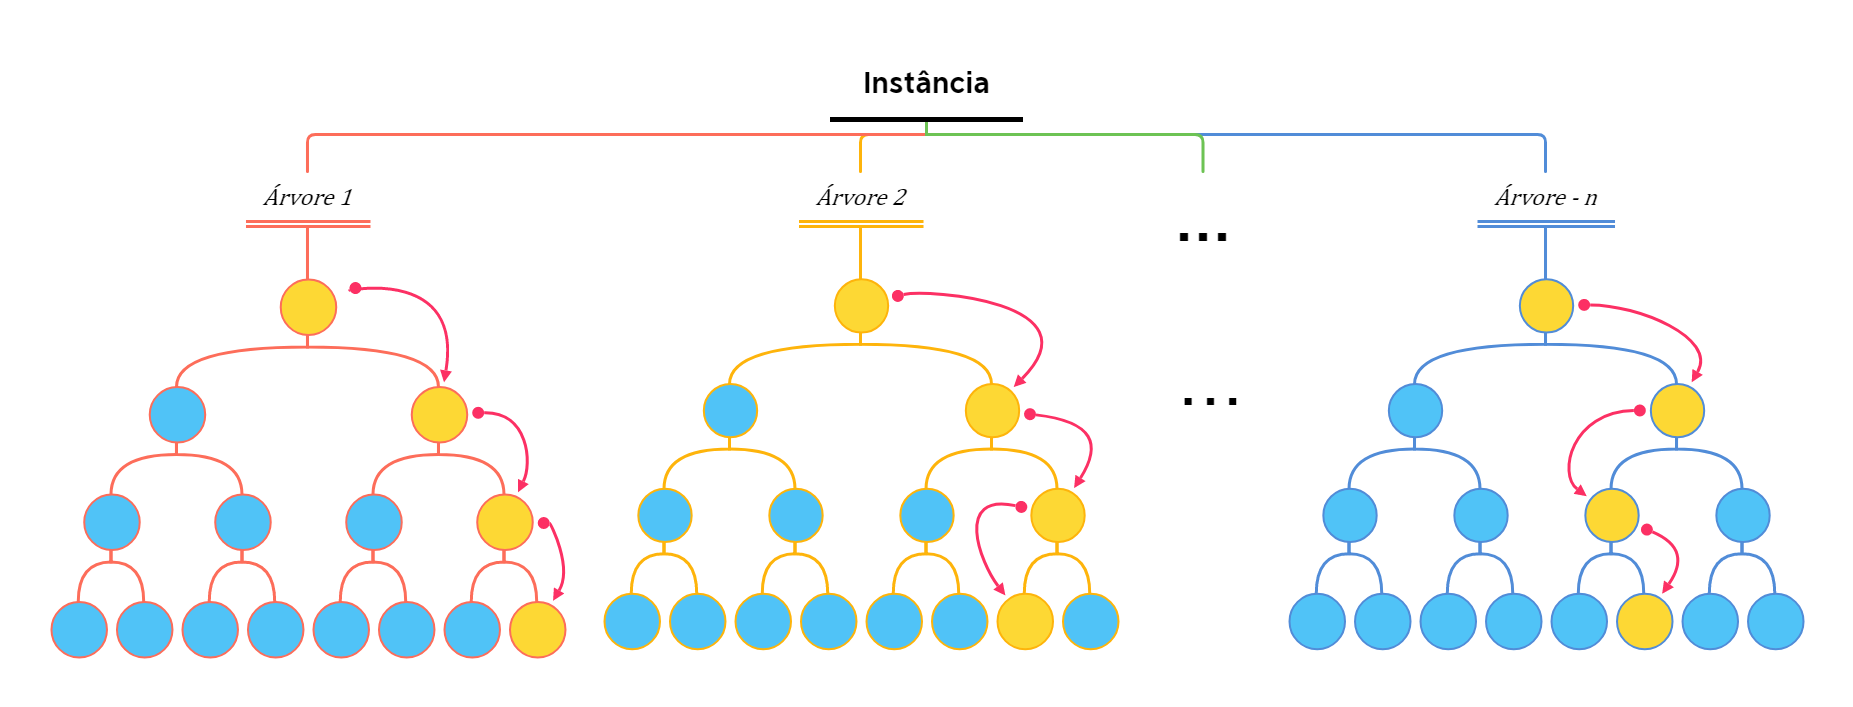
\includegraphics[width=0.9\linewidth]{Modelos/Figuras/RF}
	
	Fonte: Elaboração própria
\end{figure}


\subsubsection{Gradient Boosting (como XGBoost, LightGBM)}\label{subsubsec:lgbxgb}

O aumento de gradiente (do inglês\textit{gradient boosting}) é um método que combina vários modelos de árvore de decisão para realizar previsões. Cada uma dessas árvores de decisão é única, pois a diversidade é um elemento importante nesse processo. A diversidade é alcançada através de um processo chamado boosting, que é uma abordagem iterativa. O boosting adiciona modelos fracos ao conjunto de forma inteligente, dando mais peso aos pontos de dados que ainda não foram bem previstos. 

O processo de boosting melhora o conjunto ao focar nas partes dos dados que ainda não são compreendidas. A Figura \ref{fig:xgboost} apresenta uma visão esquemática desse processo. À medida que novos modelos fracos são adicionados, todos os modelos fracos intermediários são mantidos. O modelo final é uma combinação de todos esses modelos fracos, resultando em um ensemble que oferece uma melhor capacidade de previsão do que um único modelo.

O boosting é apenas um dos métodos de ensemble utilizados em conjunto com o bagging. O bagging também é um método que utiliza múltiplos modelos de árvore de decisão, porém, em vez de adicionar os modelos de forma iterativa, cada modelo é treinado independentemente em subconjuntos aleatórios dos dados de treinamento. Ambos os métodos, boosting e bagging, têm como objetivo melhorar o desempenho do modelo combinando as previsões de múltiplos modelos individuais.


\begin{figure}[H]
	\centering
	\caption{Impulsionando gradiente com XGBoost e LightGBM}
	\label{fig:xgboos}
	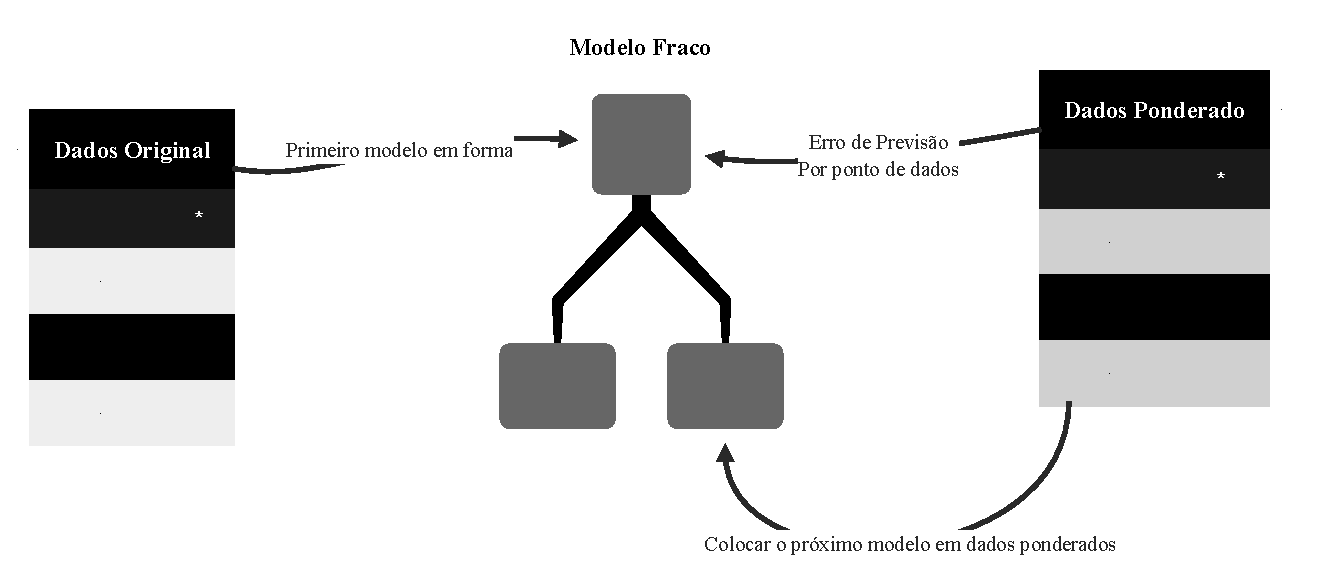
\includegraphics[width=0.9\linewidth]{Modelos/Figuras/xgboos}
	
	Fonte: Adaptação de \citeonline{korstanje2021}
\end{figure}



\subsubsection{O Gradiente em Gradiente de Boosting (Refor\c co)} \label{subsubsec:boosting}

O processo iterativo utilizado no aumento de gradiente, como descrito por \citeonline{korstanje2021}, recebe esse nome por um motivo. O termo ``gradiente'' refere-se a um campo vetorial de derivadas parciais que apontam na direção da inclinação mais acentuada. De forma simplificada, podemos pensar nos gradientes como as inclinações das estradas: quanto maior a inclinação, mais íngreme a colina. Para calcular os gradientes, são realizadas derivadas ou derivadas parciais de uma função.

No aumento de gradiente, ao adicionar árvores adicionais ao modelo, o objetivo é incorporar uma árvore que explique melhor a variação que ainda não foi explicada pelas árvores anteriores. Dessa forma, a nova árvore tem como objetivo ajustar-se aos erros ou resíduos deixados pelas árvores anteriores.

\begin{equation}
	y-\hat{y} \label{eq:xb}
\end{equation}

A equação \eqref{eq:xb} pode ser reescrita como a derivada parcial negativa da função de perda em relação às previsões $\hat{y}$:

\begin{equation}
	y-\hat{y} = -\frac{\partial L}{\partial \hat{y}} \label{eq:xb2}
\end{equation}

Isso é definido como o objetivo da nova árvore a ser adicionada no modelo de aumento de gradiente, garantindo que ela explique a máxima quantidade de variação adicional no modelo geral. Essa é a razão pela qual o modelo é chamado de "aumento de gradiente" (``\textit{gradient boosting}'', em inglês). O processo utiliza o gradiente da função de perda para guiar a adição de novas árvores, buscando minimizar o erro e melhorar a capacidade do modelo em explicar a variação nos dados.

\subsubsection{Algoritmos de boosting de gradiente}

Existem muitos algoritmos que executam versões ligeiramente diferentes de aumento de gradiente. Quando o método de aumento de gradiente foi inventado, o algoritmo não tinha um desempenho tão bom, mas isso mudou com o advento do algoritmo AdaBoost: o primeiro algoritmo capaz de se adaptar a modelos fracos.

O algoritmo de aumento de gradiente é uma das ferramentas de aprendizado de máquina com melhor desempenho no mercado. Após o AdaBoost, uma longa lista de algoritmos de aumento levemente diferentes foi adicionada à literatura, incluindo XGBoost, LightGBM, LPBoost, BrownBoost, MadaBoost, LogitBoost e TotalBoost. Ainda há muitas contribuições para melhorar a teoria do aumento de gradiente. Nesta subseção, dois algoritmos são apresentados: XGBoost e LightGBM.

O \textbf{XGBoost} é um dos algoritmos de aprendizado de máquina mais utilizados. É uma forma rápida de obter bom desempenho. Devido à sua facilidade de uso e alto desempenho, é frequentemente o primeiro algoritmo escolhido por muitos profissionais de aprendizado de máquina.

O \textbf{LightGBM} é outro algoritmo de aumento de gradiente que é importante conhecer. Atualmente, é um pouco menos difundido que o XGBoost, mas está ganhando popularidade rapidamente. A vantagem esperada do LightGBM em relação ao XGBoost é um ganho de velocidade e uma utilização mais eficiente de memória.

Nesta subseção, você encontrará as implementações de ambos os algoritmos de aumento de gradiente.

\subsubsection{A diferen\c ca entre XGBoost e LightGBM}

Se alguém planeja utilizar os dois algoritmos de aumento de gradiente, é importante que essa pessoa compreenda suas diferenças, o que também proporciona uma visão das várias divergências que existem entre os modelos disponíveis no mercado.

Uma diferença fundamental reside na maneira como esses algoritmos identificam as melhores divisões entre os nós das árvores de decisão individuais. É crucial lembrar que uma divisão em uma árvore de decisão ocorre quando a árvore precisa encontrar a separação que mais melhora o desempenho do modelo.

A abordagem intuitiva e simples para encontrar a melhor divisão é iterar por todas as possibilidades e selecionar a melhor. No entanto, essa abordagem é computacionalmente custosa, e algoritmos mais recentes apresentam alternativas mais eficientes.

Uma alternativa proposta pelo XGBoost é a segmentação baseada em histograma. Nesse caso, em vez de iterar por todas as partições possíveis, o modelo constrói um histograma para cada variável e utiliza-os para encontrar a melhor divisão geral entre as variáveis.

O LightGBM, desenvolvido pela Microsoft, adota uma abordagem mais eficiente para a definição das divisões. Essa abordagem é conhecida como amostragem unilateral baseada em gradiente (GOSS). O GOSS calcula o gradiente para cada ponto de dados e utiliza-o para filtrar os pontos de dados com gradientes baixos. Afinal, os pontos de dados com gradientes baixos já são bem compreendidos, enquanto aqueles com gradientes altos precisam ser melhor aprendidos.

O LightGBM também utiliza uma abordagem chamada Exclusive Feature Bundling (EFB), que acelera a seleção de muitas variáveis correlacionadas. Outra diferença é que o modelo LightGBM é adequado para o crescimento de folhas (leaf-wise growth), enquanto o XGBoost cultiva as árvores em níveis (level-wise growth). Essa diferença pode ser visualizada na Figura \ref{fig:xgboost}.

Essa diferença teoricamente favorece o LightGBM em termos de precisão, mas também apresenta um maior risco de overfitting (sobreajuste) quando há poucos dados disponíveis. Portanto, é importante que a pessoa considere essas distinções ao escolher entre os dois algoritmos de aumento de gradiente.

\begin{figure}[H]
	\centering
	\caption{Crescimento em folha versus crescimento em nível}
	\label{fig:xgboost}
	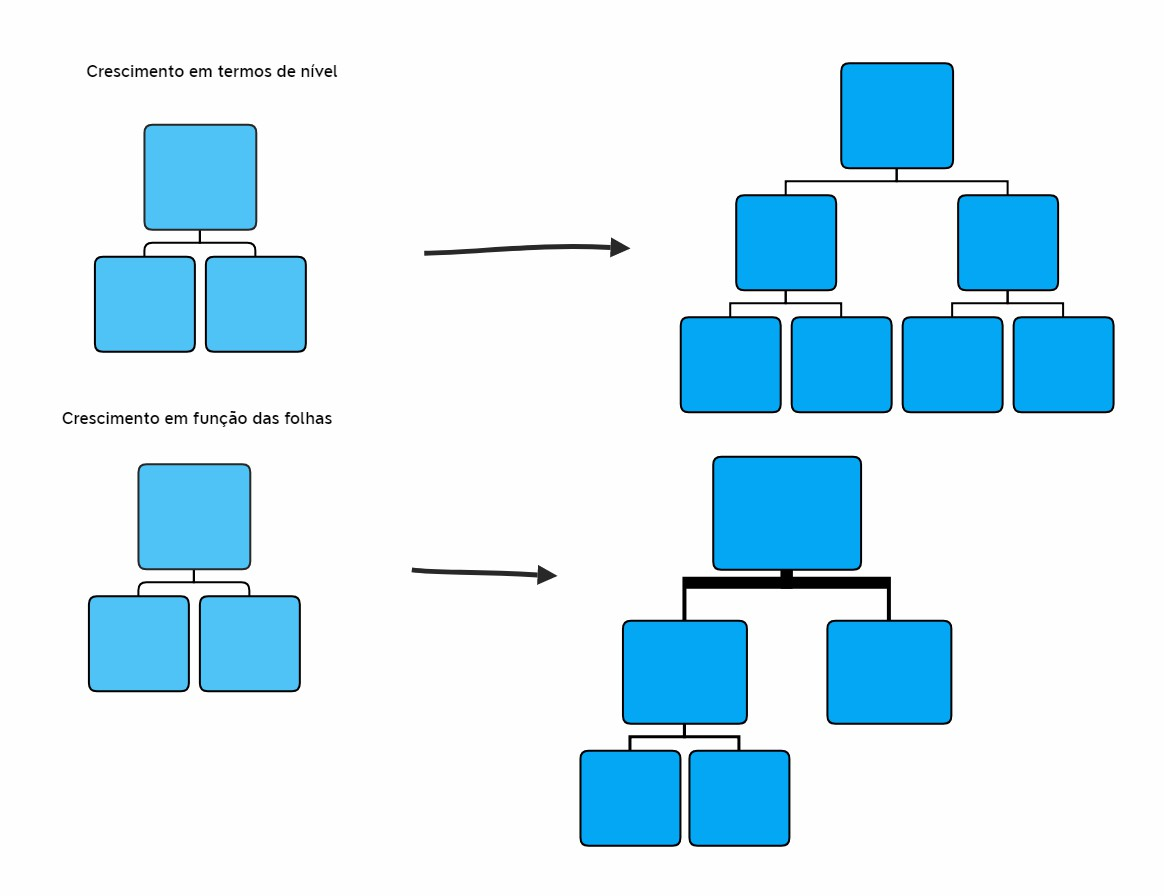
\includegraphics[width=0.9\linewidth]{Modelos/Figuras/xgboost}
	
	Fonte: Adaptação de \citeonline{korstanje2021}
\end{figure}


Na Figura \ref{fig:xgboost}, é possível visualizar como cada modelo é ajustado durante o processo de crescimento de árvore em folhas e em níveis. Essa representação gráfica oferece uma compreensão visual das diferenças entre os dois métodos.

No crescimento de árvore em folhas, como no LightGBM, novas folhas são adicionadas à árvore de forma iterativa, visando maximizar a redução do erro de treinamento. Isso significa que as árvores são expandidas adicionando folhas, uma a uma, até que o critério de parada seja alcançado.

Por outro lado, no crescimento em níveis, como no XGBoost, as árvores são expandidas em profundidade de forma simultânea em todos os níveis. Ou seja, em cada nível, todas as folhas são expandidas ao mesmo tempo, resultando em um crescimento mais uniforme da árvore.

Essa distinção no modo de crescimento das árvores pode afetar o comportamento e o desempenho do modelo. Portanto, compreender essa diferença é importante ao escolher entre esses algoritmos de aumento de gradiente.

\begin{figure}[H]
	\centering
	\caption{XGBoost e LigthGBM regressão}\label{fig:1-xgb-regressao}
	\includegraphics[width=0.9\linewidth]{Modelos/Figuras/0-xgb-regressão}
	
\end{figure}

\begin{figure}[H]
	\centering
	\includegraphics[width=0.9\linewidth]{Modelos/Figuras/0-lgbm-regressão}	
	
	
	Fonte: Elaboração própria a partir de dados da SANEPAR (2018 a 2020)
	
\end{figure}

Na Figura \ref{fig:1-xgb-regressao} é um modelo baseado nos dados coletados da SANEPAR.



\subsection{Trabalhos Relacionados}\label{subsec:estudo-de-caso-base}


A previsão da demanda de água é uma preocupação fundamental para muitas organizações e autoridades responsáveis pelo abastecimento de água. A análise de séries temporais é uma abordagem comumente usada para prever padrões futuros com base em dados históricos. Neste estudo de caso, será explorado como a análise de séries temporais pode ser aplicada para prever a demanda de água ao longo do tempo.



\subsubsection{Defini\c c\~ao do problema}



Na subseção \ref{subsubsec:obespec} estão as perguntas de pesquisa que serão abordadas no estudo de caso, da pergunta \ref{q1} à \ref{q5}, com as ramificações da \ref{q5}.

\subsubsection{Coleta de dados}


Na subseção \ref{subsec:descricao}, são apresentadas as variáveis contidas no conjunto de dados coletado no período de 2018 a 2020, durante uma grave falta de água que afetou a cidade. Devido a essa situação, foi implementado um rodízio de abastecimento de água para os residentes. Os dados foram coletados em intervalos de uma hora, levando em consideração cada variável, com ênfase na variável-alvo, denominada LT01, que representa o nível do reservatório.

O conjunto de dados possui um total de 26.306 linhas e 9 colunas. Durante a coleta dos dados, verificou-se que eles apresentam padrões sazonais, indicando variações recorrentes ao longo do tempo. Além disso, constatou-se que o consumo diário foi significativamente afetado no ano de 2020, diferindo dos anos anteriores, nos quais as mudanças não foram tão significativas.



\subsubsection{An\'alise explorat\'oria dos dados}



Ao longo do trabalho realizado, pôde-se observar na subseção \ref{subsec:detec} que foi realizada uma análise gráfica do problema antes da aplicação de qualquer método. A detecção de anomalias mostrou-se desafiadora, porém não impossível de ser realizada. Essa detecção permitiu a análise da presença de sazonalidade nos dados. A decomposição STL foi utilizada para essa finalidade, conforme descrito na etapa \ref{etp:3} e detalhado na subseção \ref{subsubsec:stl}, onde são apresentadas as decomposições realizadas.

É fundamental lembrar que, durante a análise exploratória, os dados sofreram algumas alterações. Por exemplo, a média diária foi calculada em vez de ser considerada a nível horário, resultando em uma redução do conjunto de dados de 26.306 linhas para 1.096 linhas. A decomposição STL foi aplicada nos formatos aditivo e multiplicativo, e ambas as abordagens estão ilustradas nas Figuras \ref{fig:stl-aditiva} e \ref{fig:stl}, respectivamente.

Adicionalmente, na subseção \ref{subsubsec:stl}, foi realizada a verificação da estacionariedade da série. O teste de Dickey-Fuller (DF) foi empregado para auxiliar na tomada de decisões, e os resultados demonstraram que a série em análise é estacionária, conforme evidenciado pelo teste DF.



\subsubsection{Escolha do modelo}



Dentro da análise, foram incluídos uma variedade de modelos para melhor capturar a natureza dos dados e aprimorar as previsões. Esses modelos incluem:

\begin{description}
	\item [RNN (Rede Neural Recorrente),] que leva em conta as dependências sequenciais nos dados para prever valores futuros.

	\item [LSTM (Long Short-Term Memory),] um tipo de RNN que lida especialmente bem com sequências longas e dependências de longo prazo.

	\item [GRU (Gated Recurrent Unit),] outra variante de RNN que equilibra o poder de modelagem e a eficiência computacional.

	\item [Transformer,] um modelo amplamente utilizado para tarefas de processamento de linguagem natural e sequências, que também pode ser adaptado para previsões sequenciais.

	\item [Prophet,] um modelo de previsão desenvolvido pelo Facebook que lida bem com dados sazonais e tendências.

	\item [Decision Tree Regressor,] um modelo baseado em árvore de decisão que segmenta os dados em subgrupos para fazer previsões.

Esses modelos são complementados com abordagens tradicionais como:

	\item [Modelos de séries temporais univariados,] incluindo AR, MA, ARMA, ARIMA e SARIMA, que levam em consideração a sazonalidade dos dados.

	\item [Modelos de séries temporais multivariados,] como ARX, ARIMAX e SARIMAX, que incorporam variáveis exógenas para melhorar as previsões.

Além disso, foram explorados modelos de aprendizado de máquina supervisionados:

	\item [LR (\textit{Regressão Linear}),] que estabelece relações lineares entre variáveis para fazer previsões.

	\item [RFR (\textit{Random Forest Regressor}),] um \textit{ensemble} de árvores de decisão que captura complexas relações nos dados.

	\item [LightGBM e XGBoost,] modelos baseados em \textit{gradient boosting} que são reconhecidos por sua eficácia na previsão e tomada de decisões. O XGBoost é particularmente conhecido por seu desempenho superior em várias métricas de avaliação.

\end{description}

A inclusão desses modelos permite uma abordagem abrangente à previsão, aproveitando as vantagens específicas de cada método para lidar com diferentes aspectos dos dados e melhorar as previsões em um conjunto diversificado de cenários.



\subsubsection{Divis\~ao dos dados}


Para obter a divisão mais adequada dos dados, verificam-se a média e o desvio padrão de cada um desses conjuntos. O conjunto de dados é dividido em três partes: treinamento, validação e teste. Nessa divisão, utiliza-se inicialmente 70\% dos dados para treinamento e validação, e os 30\% restantes para teste. Em seguida, a porção de treinamento e validação é subdividida em 80\% para treinamento e 20\% para validação.

\subsubsection{Ajuste do modelo}
Nesta etapa, você aplicará o modelo selecionado aos dados de treinamento. Ajuste os parâmetros do modelo com o objetivo de minimizar os erros de previsão. Dependendo do modelo escolhido, você pode usar técnicas de otimização para encontrar os melhores parâmetros.

Ao ajustar o modelo para a base de dados, foi feita uma alteração na ordem do modelo sugerido pelo pmdarima. A escolha foi trocar o modelo SARIMAX(1,1,1)(2,1,0,12) para SARIMAX(7,1,7)(2,1,0,12). Essa decisão foi tomada com base na observação de um ajuste mais preciso aos dados, evidenciado pela redução nos resíduos e uma melhor captura das características da série temporal. Além disso, considerando o conhecimento do problema e as características específicas dos dados, foi identificado que padrões mais complexos requeriam ordens mais altas para serem adequadamente capturados. Dessa forma, foi realizado um processo iterativo de experimentação e avaliação para determinar o modelo SARIMAX(7,1,7)(2,1,0,12) como o mais adequado para a base de dados em questão. É importante ressaltar que o desempenho do novo modelo será avaliado por meio de diagnósticos adicionais e análise dos resultados obtidos.

Os modelos RNN, LSTM e GRU foram ajustados minuciosamente por meio da técnica de otimização de hiperparâmetros do Optuna, permitindo uma exploração adaptativa e eficiente do espaço de configurações. Essa abordagem exclusiva do Optuna resultou em modelos sequenciais com aprimoramento notável na capacidade preditiva. Parâmetros vitais, como taxa de aprendizado, tamanho da camada oculta e número de unidades, foram otimizados de forma eficaz através do Optuna.

O Random Forest Regressor (RFR) apresentou melhorias notáveis após o ajuste com o Optuna. A otimização realizada pelo Optuna permitiu identificar uma combinação de hiperparâmetros ideal para o RFR, resultando em um significativo aprimoramento no desempenho preditivo desse modelo.

No entanto, o modelo Transformer e o Prophet não puderam ser otimizados com sucesso por meio do Optuna. Apesar das tentativas de ajuste, as melhorias significativas não foram observadas em seus resultados. Estes modelos mantiveram suas configurações padrão, uma vez que os esforços de otimização com o Optuna não resultaram em ganhos substanciais.

Considerando que o modelo LR (Regressão Linear) não demonstrou melhorias significativas, uma decisão foi tomada para substituí-lo pelo modelo Decision Tree Regressor. Este último foi ajustado empregando o Optuna, buscando encontrar a configuração de hiperparâmetros ideal para o modelo de árvore de decisão. Essa decisão foi respaldada pelo fato de que o Optuna havia demonstrado ser uma ferramenta eficaz para otimização de hiperparâmetros, como evidenciado pelas melhorias observadas no RFR e em outros modelos.

Dessa forma, os modelos RNN, LSTM, GRU, XGBRegressor, LGBMRegressor e o Decision Tree Regressor foram todos otimizados com sucesso utilizando o Optuna, resultando em previsões mais robustas e confiáveis. No entanto, os modelos Transformer e Prophet mantiveram suas configurações originais devido à ausência de melhorias substanciais após tentativas de otimização com o Optuna.

O \textbf{Optuna} oferece uma abordagem de otimização de hiperparâmetros mais avançada e eficaz em comparação com outras técnicas amplamente utilizadas, como o GridSearchCV, BayesSearchCV e RandomizedSearchCV. Enquanto essas abordagens tradicionais têm suas vantagens, o Optuna leva a otimização de hiperparâmetros a um nível superior.

O \textbf{GridSearchCV}, por exemplo, é uma técnica exaustiva que explora todas as combinações possíveis de hiperparâmetros. Embora seja abrangente, essa abordagem pode se tornar computacionalmente intensiva e demorada, especialmente quando o espaço de busca é grande. Além disso, o GridSearchCV não considera a interação entre os hiperparâmetros, o que pode limitar sua capacidade de encontrar combinações ótimas.

O \textbf{BayesSearchCV} melhora a eficiência em relação ao GridSearchCV usando otimização bayesiana, mas ainda enfrenta limitações. Ele utiliza um processo de amostragem sequencial com um modelo probabilístico para explorar o espaço de hiperparâmetros de maneira mais inteligente. No entanto, o BayesSearchCV ainda pode exigir muitas iterações para encontrar configurações ideais, especialmente em espaços de busca complexos.

O \textbf{RandomizedSearchCV}, por outro lado, busca aleatoriamente subconjuntos do espaço de hiperparâmetros. Isso pode ser útil para espaços de busca vastos, mas ainda não garante uma exploração eficaz do espaço para encontrar as melhores configurações.

Aqui é onde o Optuna se destaca. Utilizando algoritmos avançados de otimização, o Optuna oferece uma abordagem mais inteligente e eficiente para encontrar as configurações ideais de hiperparâmetros. Ele emprega técnicas de amostragem adaptativa, como o algoritmo TPE (Tree-structured Parzen Estimator), para direcionar a pesquisa para as áreas mais promissoras do espaço de hiperparâmetros. Isso permite uma exploração mais eficaz e uma descoberta mais rápida das configurações que maximizam a métrica de avaliação.

Além disso, o Optuna é altamente flexível e pode ser facilmente integrado a diversos algoritmos e frameworks de aprendizado de máquina. Sua abordagem adaptativa e inteligente proporciona economia de recursos computacionais e, ao mesmo tempo, aumenta as chances de encontrar configurações de hiperparâmetros que levem a um desempenho superior do modelo.

Em resumo, o Optuna supera as abordagens tradicionais, como o GridSearchCV, BayesSearchCV e RandomizedSearchCV, oferecendo uma otimização de hiperparâmetros mais eficiente, inteligente e adaptativa. Sua capacidade de explorar de maneira direcionada o espaço de hiperparâmetros resulta em uma descoberta mais rápida das configurações ideais, impulsionando o desempenho dos modelos de aprendizado de máquina de forma significativa.

\subsubsection{Avalia\c c\~ao do modelo}


A avaliação da precisão dos modelos de previsão é uma etapa fundamental no processo de modelagem. Diversas métricas podem ser utilizadas para esse propósito, como o sMAPE, o MAE e o RRMSE. Essas métricas têm sido amplamente adotadas na literatura de previsão e são consideradas indicadores confiáveis para mensurar a qualidade das previsões.

De acordo com \citeonline{zhang2016}, o MAPE é uma métrica bastante utilizada na avaliação de modelos de previsão, especialmente quando há variações significativas nos dados ou quando se deseja comparar a precisão de diferentes modelos. O MAPE calcula o erro médio percentual entre as previsões e os valores reais, fornecendo uma medida relativa da precisão do modelo.

De acordo com \citeonline{willmott2005advantages}, o uso do erro médio absoluto (MAE) apresenta vantagens na avaliação do desempenho médio de um modelo, em comparação com o erro quadrático médio (RMSE).

\citeonline{jones2017} destacam a importância do RMSE na avaliação de modelos e argumentam contra a exclusão dessa métrica na literatura.


O RRMSE é uma métrica de avaliação altamente eficaz para medir a precisão relativa de modelos de regressão. Eles destacam que sua normalização em relação à média dos valores reais permite uma interpretação intuitiva e facilita a comparação entre diferentes modelos. Segundo os autores, o RRMSE é amplamente utilizado na literatura devido à sua capacidade de fornecer uma medida robusta e padronizada da precisão dos modelos de regressão \cite{lopes2020evaluation}. Segundo \citeonline{peng2017effective}, o MAPE é amplamente utilizado na avaliação de modelos de previsão, especialmente quando há variações significativas nos dados ou quando se deseja comparar a precisão de diferentes modelos.

O sMAPE é uma métrica amplamente utilizada para avaliar a precisão de modelos de previsão. Eles afirmam que o sMAPE possui algumas vantagens, como a consideração da simetria dos erros percentuais e a interpretação intuitiva como uma medida de precisão relativa \cite{nguyen2020toxicological}.

Além disso, \citeonline{jones2017} afirmam que o MAE e o RMSE são métricas amplamente adotadas na análise de previsões, pois fornecem uma medida direta do desvio absoluto e do desvio quadrático médio entre as previsões e os valores observados. O MAE é particularmente útil quando se busca uma medida de erro que não seja sensível a valores extremos, enquanto o RMSE penaliza de forma mais significativa os erros maiores, oferecendo uma visão mais abrangente da precisão do modelo.

O sMAPE é uma métrica de avaliação popular para comparar a precisão de diferentes modelos de previsão. Eles destacam que o sMAPE é particularmente útil quando os valores de demanda têm diferentes magnitudes, pois captura os erros relativos em uma escala percentual. Além disso, o sMAPE possui uma interpretação intuitiva e facilita a comparação entre modelos de previsão \cite{hyndman2006effect}.


Portanto, ao utilizar essas métricas, o pesquisador estará seguindo uma prática comum e fundamentada na literatura. O sMAPE permitirá avaliar a precisão relativa das previsões, enquanto o MAE e o RRMSE fornecerão uma medida direta dos desvios absolutos e quadráticos, respectivamente. Essas métricas fornecerão uma base sólida para a avaliação dos modelos de previsão utilizados na pesquisa.


\subsubsection{Previs\~oes Futuras}


Com base nos modelos AR, ARX, MA, ARMA, ARIMA, ARMAX, SARIMA, SARIMAX,  XGBRegressor, LGBMRegressor, RNN, LSTM, GRU, Transformer, Prophet e Decision Tree Regressor, que foram cuidadosamente aplicados e avaliados, é possível afirmar que uma vez que a precisão desses modelos tenha sido satisfatória, eles podem ser utilizados para fazer previsões futuras. Ao aplicar esses modelos aos dados futuros disponíveis, ele poderá estimar a demanda de água para diferentes horizontes de previsão, como um dia, uma semana, duas semanas e um mês.

Essas previsões fornecerão informações valiosas para o planejamento e gerenciamento eficiente dos recursos hídricos. Ao ter conhecimento antecipado da demanda de água esperada nos próximos períodos, será possível adotar medidas adequadas para garantir o suprimento apropriado de água, prevenir escassez ou desperdício e realizar um planejamento eficaz para a distribuição e uso dos recursos hídricos.

Com base nos resultados significativos obtidos por esses modelos durante o processo de validação, o pesquisador terá confiança em aplicá-los para previsões futuras de curto prazo. Essas previsões permitirão a compreensão das tendências e variações na demanda de água ao longo de diferentes períodos, capacitando os responsáveis pela gestão dos recursos hídricos a tomar decisões informadas e estratégicas.

Portanto, uma vez que os modelos tenham sido devidamente avaliados e demonstrado sua eficácia, eles podem ser utilizados para fazer previsões precisas da demanda de água em horizontes de previsão de um dia, uma semana, duas semanas e um mês, contribuindo para a gestão e planejamento eficiente dos recursos hídricos.

\subsubsection{Monitoramento e Ajuste Cont\'inuo}


É importante destacar que todas as questões de pesquisa abordadas neste estudo estão fundamentadas no fator dos horários de pico e nas anomalias que ocorreram durante o período analisado. O comportamento da demanda de água durante os horários de maior consumo e as anomalias observadas foram aspectos-chave que motivaram a realização desta pesquisa.

Ao investigar os efeitos dos horários de pico e das anomalias na demanda de água, o estudo teve como objetivo compreender melhor os padrões de consumo, identificar possíveis causas para as variações significativas na demanda e desenvolver modelos de previsão mais precisos. A análise desses aspectos contribuiu para uma melhor compreensão dos desafios enfrentados no abastecimento de água e na gestão dos recursos hídricos durante os períodos críticos.

Considerando a importância desses fatores na formulação das questões de pesquisa, as análises realizadas e os modelos desenvolvidos buscaram fornecer insights e informações relevantes para aprimorar a capacidade de previsão e planejamento do abastecimento de água, especialmente durante os horários de pico e diante de anomalias observadas.

\subsubsection{Principais Conclus\~ao}


Ao longo deste estudo de caso, foram resolvidas as questões de pesquisa levantadas por meio da aplicação da análise de séries temporais para prever a demanda de água. A abordagem adotada demonstrou ser eficaz na obtenção de insights valiosos para o gerenciamento do abastecimento hídrico.

Foi constatado que a análise de séries temporais é uma ferramenta promissora para prever a demanda de água, permitindo tomar decisões informadas e embasadas nesse contexto. Por meio da modelagem e aplicação de diversos modelos, como ARIMA, SARIMA e outros, foi possível analisar e interpretar os dados históricos de maneira precisa, obtendo previsões confiáveis.

Durante o estudo, foram levantadas questões relacionadas à sazonalidade da demanda de água, influência de fatores externos imprevisíveis e mudanças no comportamento dos consumidores. Através da adaptação das técnicas de análise de séries temporais, foi possível abordar essas questões de forma eficiente e obter respostas relevantes para o gerenciamento do abastecimento de água.

Ao longo do processo, foram identificadas anomalias e flutuações na demanda de água, bem como tendências sazonais específicas. Por meio da análise dos resultados obtidos com os modelos aplicados, foi possível ajustar e aprimorar as previsões, tornando-as mais acuradas e confiáveis.

Em suma, este estudo de caso demonstrou que a análise de séries temporais é uma abordagem eficaz para prever a demanda de água, permitindo uma gestão mais eficiente do abastecimento hídrico. Ao adaptar e aplicar as técnicas adequadas aos dados específicos e às características do contexto, foram resolvidas as questões de pesquisa propostas e obtidos resultados significativos.

Essas descobertas têm o potencial de contribuir para a tomada de decisões embasadas no planejamento e no gerenciamento da demanda de água, visando a sustentabilidade e a eficiência dos recursos hídricos.

\section{Resultados} \label{sec:result}

Neste capítulo, é fornecida uma síntese e uma visão geral dos resultados obtidos até o momento. É apresentado um resumo sucinto das principais realizações e descobertas que foram alcançadas até agora.


\subsection{Planejamento do Problema} \label{subsec:planexp}

Assim como apresentado na seção \ref{subsubsec:etp}, os passos da dissertação delinearam o processo pelo qual cada modelo foi construído e os métodos utilizados para responder às questões de pesquisa abordadas na seção \ref{subsubsec:obespec}. Esses passos proporcionaram uma cronologia lógica das etapas realizadas ao longo do tempo com os dados da SANEPAR, ilustrando o progresso e os resultados alcançados até o momento.


\subsubsection{An\'alise Explorat\'oria dos dados (EDA)}

A partir do passo \ref{etp:1}, foi realizado o EDA (Exploratory Data Analysis) para processar os dados obtidos até o momento. O EDA permite responder às questões de pesquisa levantadas. Conforme mencionado por \citeonline{Yu2016}, na era dos grandes dados, é desafiador descobrir as regras, modelos analíticos e hipóteses por trás dos volumes massivos de dados caóticos, não estruturados e multimídia coletados por meio de vários canais. A análise exploratória de dados foi promovida por John Tukey como uma abordagem para explorar os dados, resumir suas principais características e formular hipóteses que possam direcionar a coleta adicional de dados e experimentos. No contexto de grandes análises de dados, várias técnicas de EDA têm sido adotadas.

Ao analisar a pergunta \ref{q1}, que relaciona a demanda com a variável prevista e a pressão para a variável PT01, pode-se observar na Figura \ref{fig:person} que ambas as variáveis apresentam uma correlação quase perfeita, com um coeficiente de correlação de Pearson ($r$) igual a 1. Portanto, para responder a essa pergunta, basta observar a correlação de Pearson na Figura \ref{fig:person}.

Para responder à pergunta \ref{q2}, é criada uma tabela para fornecer uma resposta mais completa.


\begin{table}[!htb]
	\centering
	\caption{Descrição estatística dos dados com o filtro aplicado das 18h às 21h}\label{tb:est}
	\begin{tabular}{@{}cccccccccc@{}}
		\toprule
		\textbf{18 a 21h}  & \textbf{B1} & \textbf{B2} & \textbf{B3} & \textbf{LT01} & \textbf{FT01} & \textbf{FT02} & \textbf{FT03} & \textbf{PT01} & \textbf{PT02} \\ \midrule
		\textbf{Contagem} & 4385    & 4385     & 4385     & 4385      & 4385       & 4385       & 4385       & 4385       & 4385       \\
		\textbf{Média}      & 51,94       & 27,81       & 6,41        & 3,24          & 112,68        & 132,93        & 112,41        & 4,11          & 20,80         \\
		\textbf{STD}       & 17,14       & 17,61       & 16,77       & 0,70          & 132,59        & 44,78         & 31,33         & 0,76          & 6,14          \\
		\textbf{Min}       & 0           & 0           & 0           & 0,29          & 0             & 0             & 0             & 0,88          & 0             \\
		\textbf{25\%}      & 57,84       & 0           & 0           & 2,79          & 0,12          & 123,96        & 111,66        & 3,62          & 21,72         \\
		\textbf{50\%}      & 57,99       & 34,91       & 0           & 3,30          & 0,12          & 136,00        & 118,82        & 4,15          & 22,05         \\
		\textbf{75\%}      & 57,99       & 38,02       & 0           & 3,78          & 264,27        & 148,20        & 125,63        & 4,66          & 23,02         \\
		\textbf{Max}       & 59,99       & 59,99       & 59,99       & 4,40          & 383,87        & 326,17        & 194,35        & 5,68          & 28,08         \\ \bottomrule
	\end{tabular}
	
	\fonte{Elaboração própria a partir de dados da SANEPAR (2018 a 2020)}
\end{table}



Na Tabela \ref{tb:est}, o desvio padrão é representado pela sigla STD, que corresponde à expressão em inglês ``\textit{standard deviation}''. Além disso, em resposta à pergunta \ref{q2}, é importante mencionar que, assim como em qualquer empresa de tratamento de água, é utilizado um mecanismo de acionamento automático chamado "trava de segurança" para evitar que o nível do tanque chegue a zero e haja falta de água nos locais abastecidos por esse tanque. O nível mínimo que o tanque pode alcançar é de $5.29 m^3$ (equivalente a 5,29 litros). As bombas são ativadas em sua potência máxima para evitar que sejam acionadas quando o nível do tanque. No entanto, a bomba 1 ainda estaria operando para completar o nível do tanque caso ele esteja dentro dessa faixa.

Em situações de demanda de pico, uma abordagem ideal, embora não necessariamente a mais econômica, seria ter um tanque de reserva adicional e instalar uma tubulação que os conecte. Durante o dia, ambos os tanques seriam abastecidos e, à noite, por meio da ação da gravidade, eles manteriam o mesmo nível até que o consumo atinja um ponto em que as bombas sejam acionadas. Essa estratégia permite um abastecimento contínuo e eficiente de água.


Na pergunta \ref{q3}, observa-se que o tanque tem uma capacidade máxima de $4,256 m^3$, o que equivale a $4.256$ litros. Para atender a essa demanda e manter o tanque quase cheio ou sempre cheio, é necessário que o fluxo de entrada esteja na faixa de $[238, 302] \ m^3/h$, o fluxo de gravidade esteja entre $[126, 182] \ m^3/h$, o fluxo de retorno esteja entre $[110, 144] \ m^3/h$, a pressão de sucção esteja entre $[1.92, 4.24] \ mca$ e a pressão de retorno esteja entre $[21, 24] \ mca$.

Para responder à pergunta \ref{q4}, o ponto de equilíbrio, onde as bombas não precisam ser acionadas, ocorre quando o fluxo de FT01 é de $211 \ m^3/h$, FT02 é de $114 \ m^3/h$, FT03 é de $100 \ m^3/h$ e o nível do tanque está em $3.545 \ m^3$.
No que diz respeito à pergunta \ref{q5}\ref{q5:a}, o nível do tanque deve ser de $4,00 \ m^3$ para evitar o funcionamento das bombas durante as horas de pico.

\subsubsection{M\'ultiplas entradas e sa\'ida \'unica (MISO)}

Nesta \ref{etp:2} os modelos que foram mais cobertos no decorrer da dissertação são os modelos ARIMA ou aqueles derivados deste modelo e os modelos regressivos fora do LR têm múltiplas entradas e uma saída da variável que se prevê a LT01, as outras variáveis servem como suporte para melhorar os modelos do tipo ARX ou modelos com variáveis exógenas. Os modelos ARIMA sem a variável exógena são apenas uma entrada semelhante com LR.

\subsubsection{Decomposi\c c\~ao STL}\label{subsubsec:stl}

A decomposição sazonal e de tendência utilizando o procedimento de Loess (STL) é uma técnica amplamente utilizada para decompor séries temporais em seus componentes sazonais, de tendência e restantes. De acordo com \citeonline{Theodosiou20111178}, o método STL realiza a decomposição aditiva dos dados por meio de uma sequência de aplicações do Loess mais suave, onde regressões polinomiais ponderadas localmente são aplicadas em cada ponto do conjunto de dados, tendo como variáveis explicativas os valores mais próximos do ponto cuja resposta está sendo estimada.

A decomposição STL é especialmente útil para identificar e isolar padrões sazonais e de tendência presentes nas séries temporais. Ela permite a separação dos componentes sazonais, que ocorrem em intervalos regulares ao longo do tempo, da componente de tendência, que indica a direção geral dos dados ao longo do tempo. A decomposição também resulta em uma componente restante, que representa a variação não explicada pelos componentes sazonais e de tendência.

Ao aplicar a decomposição STL, a série temporal pode ser expressa como a soma dos componentes sazonais, de tendência e restantes. Essa técnica é útil para análise e modelagem de séries temporais, pois proporciona uma compreensão mais clara dos padrões de variação presentes nos dados.

A decomposição STL é formalmente definida como:

\begin{eqnarray}
	y_t=f\left(S_t, T_t, R_t\right)&=&\left\{\begin{array}{l}
		y_t=S_t+T_t+R_t \quad \text { aditivo } \\
		y_t=S_t T_t R_t \quad \text { multiplicativo }
	\end{array}\right. \label{eq:stl}
\end{eqnarray}

\begin{figure}[!htb]
	\centering
	\caption{Decomposição STL}
	\begin{subfigure}{1\textwidth}
		\includegraphics[width=\linewidth]{"Resultados/Figuras/STL aditiva"}
		\caption{Decomposição STL aditiva dos dados coletados}
		\label{fig:stl-aditiva}
	\end{subfigure}
		
	\begin{subfigure}{1\textwidth}
		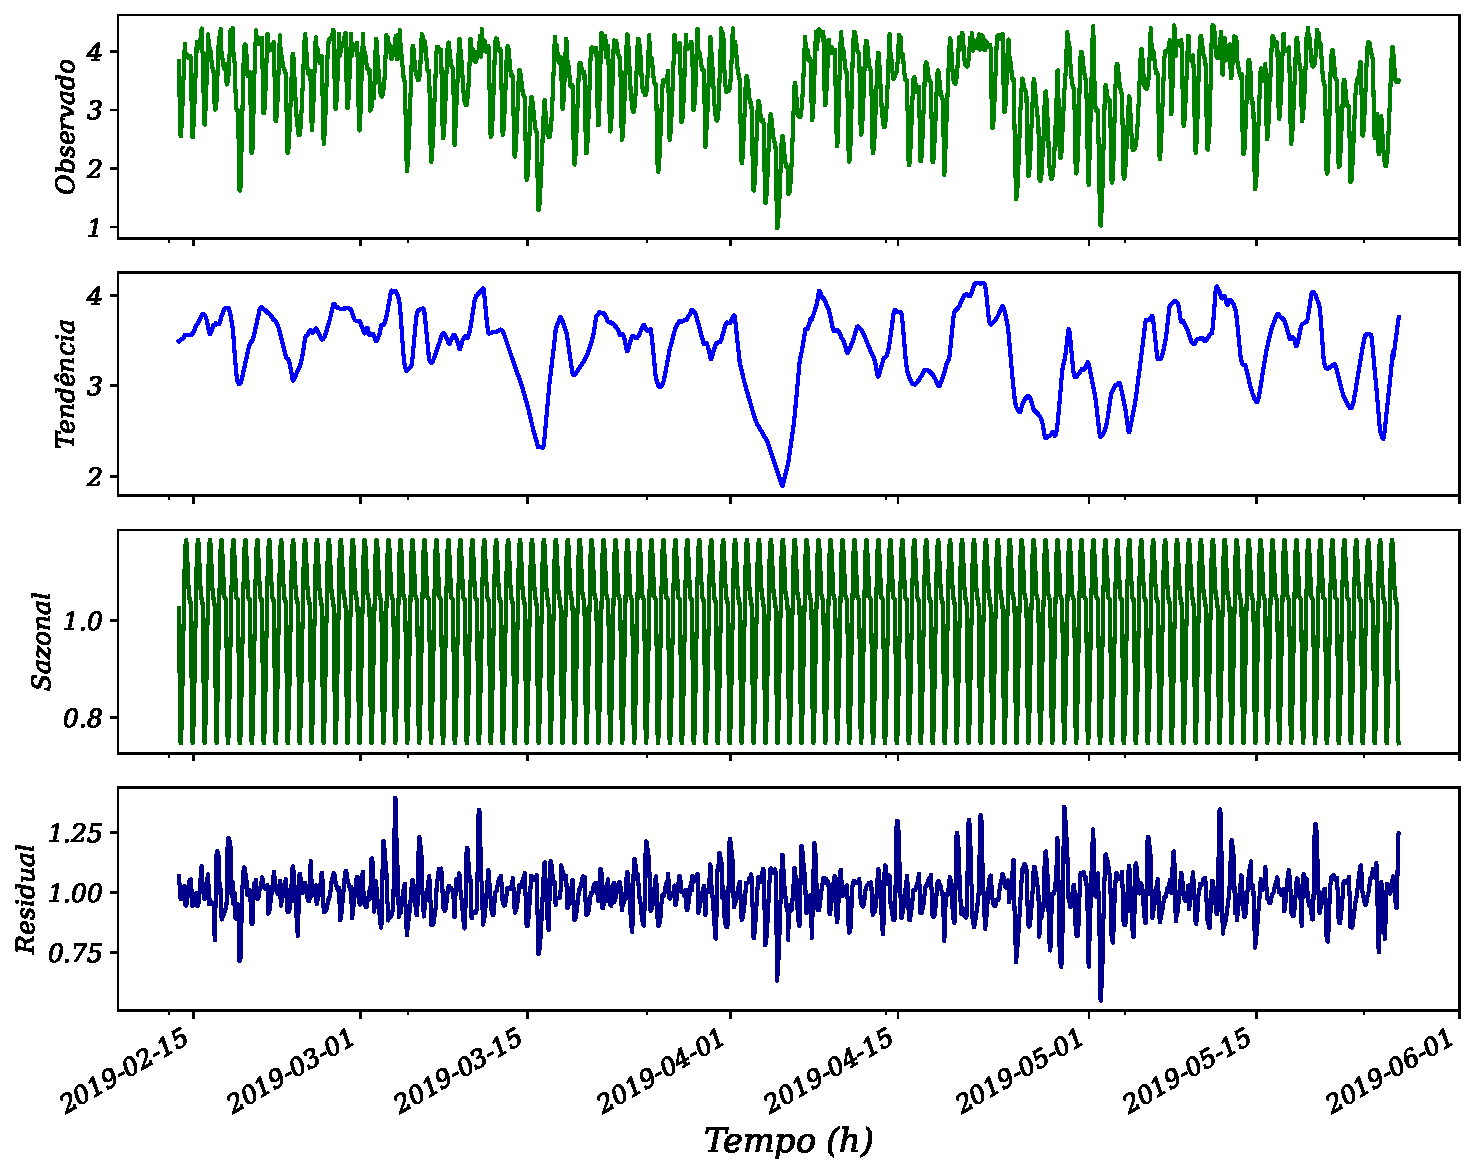
\includegraphics[width=\linewidth]{Resultados/Figuras/STL}
		\caption{Decomposição STL multiplicativa dos dados coletados}
		\label{fig:stl}
	\end{subfigure}
	
	\fonte{Elaboração própria a partir de dados da SANEPAR (2018 a 2020)}
\end{figure}

Na resposta à pergunta \ref{q5}\ref{q5:b}, as Figuras \ref{fig:stl-aditiva} e \ref{fig:stl} fornecem informações sobre a presença de tendência, sazonalidade e resíduos na série temporal.

Através da decomposição, é possível analisar se a série apresenta tendência, sazonalidade e resíduos. Ao observar as Figuras \ref{fig:stl-aditiva} e \ref{fig:stl}, é evidente que os dados exibem ambos os padrões. Isso indica que a série é estacionária, como confirmado pelo seguinte teste.

Teste de Dickey-Fuller (DF) Aumentado:
\begin{itemize}
	\item Estatística de teste ADF: $-4,25$
	\item Valor de p: $0,001$
	\item Atrasos utilizados: $21$
	\item Observações: $1074$
	\item Valor crítico ($1\%$): $-3,44$
	\item Valor crítico ($5\%$): $-2,86$
	\item Valor crítico ($10\%$): $-2,57$
\end{itemize}

Com base na forte evidência contra a hipótese nula, podemos rejeitar a hipótese nula. Isso indica que os dados não possuem raiz unitária e são estacionários em \ref{q5}\ref{q5:c}. Identificar as horas de pico entre 18h e 21h não é uma tarefa fácil. No entanto, ao observar a Figura \ref{fig:hist}, podemos notar um aumento na demanda durante essas horas durante o ano de 2020.
	
	
	\begin{figure}[!htb]
		\centering
		\caption{Violino no nível do reservatório}
		\label{fig:hist}
		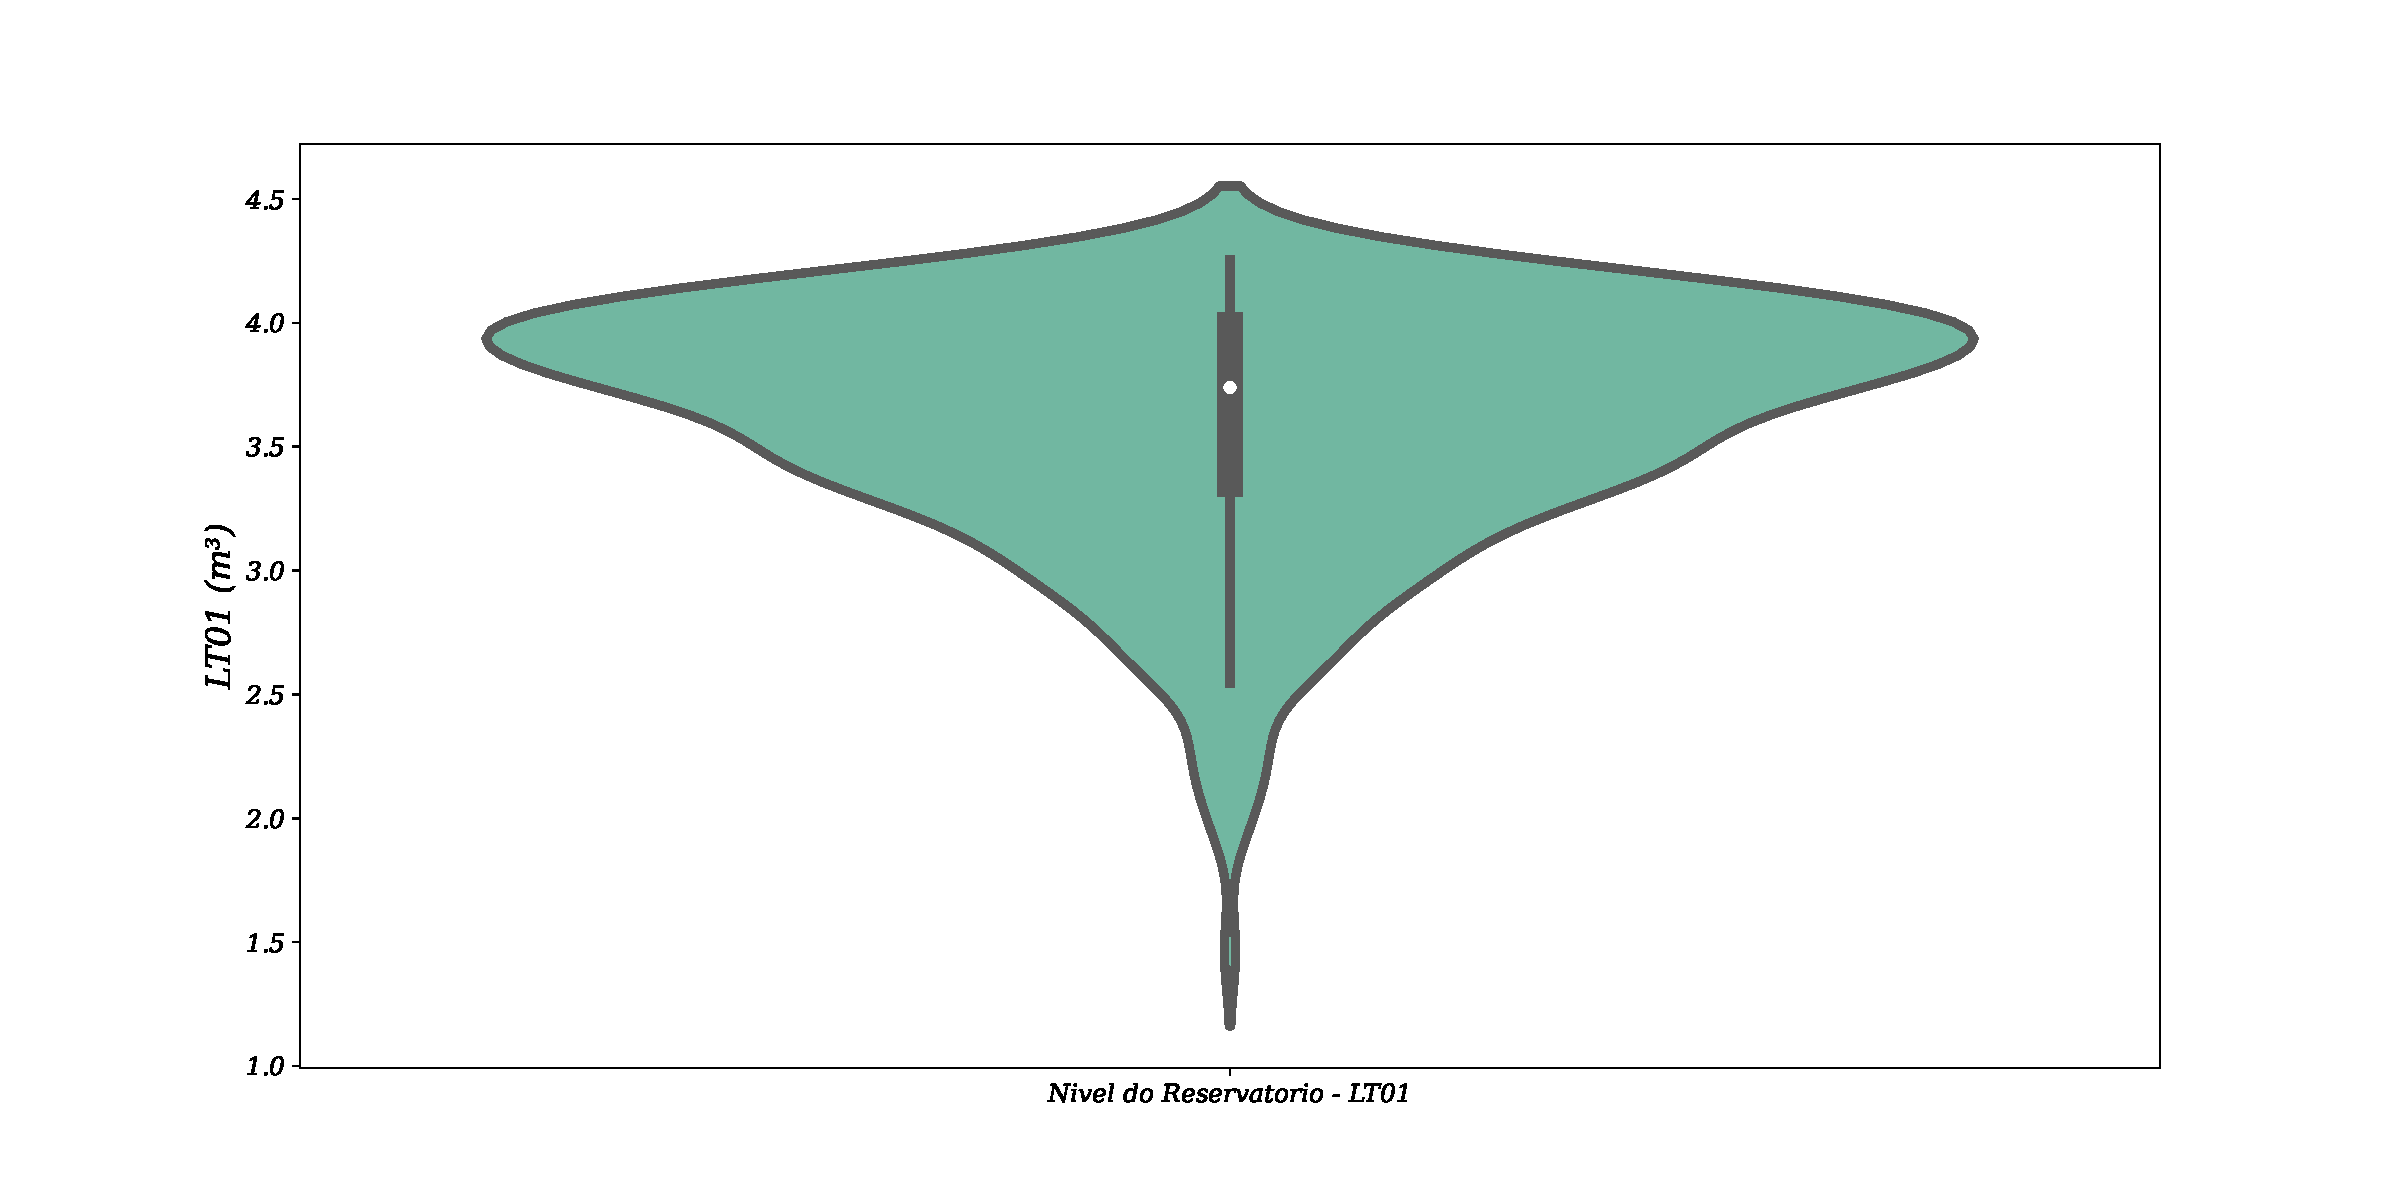
\includegraphics[width=0.9\linewidth]{Resultados/Figuras/viol}
		
		\fonte{Elaboração própria a partir de dados da SANEPAR (2018 a 2020)}
	\end{figure}
	
Conforme mencionado na subseção \ref{subsubsec:motivacao}, as anomalias climáticas ocorridas em 2020, especialmente a falta de chuvas, tiveram um impacto significativo nos resultados. Isso contribuiu para as mudanças observadas na demanda de água ao longo desse período.

Com relação à pergunta \ref{q5}\ref{q5:d}, durante as horas de pico, é necessário que o nível do tanque esteja dentro da faixa de $[3.545,4.256] m^3$ para evitar o acionamento das bombas. Manter o nível do tanque dentro dessa faixa permitirá que o sistema opere de forma eficiente, atendendo à demanda sem a necessidade de acionar as bombas.
	
	
	\begin{figure}[!htb]
		\centering
		\caption{Violino da vazão de recalque}
		\label{fig:ft03}
		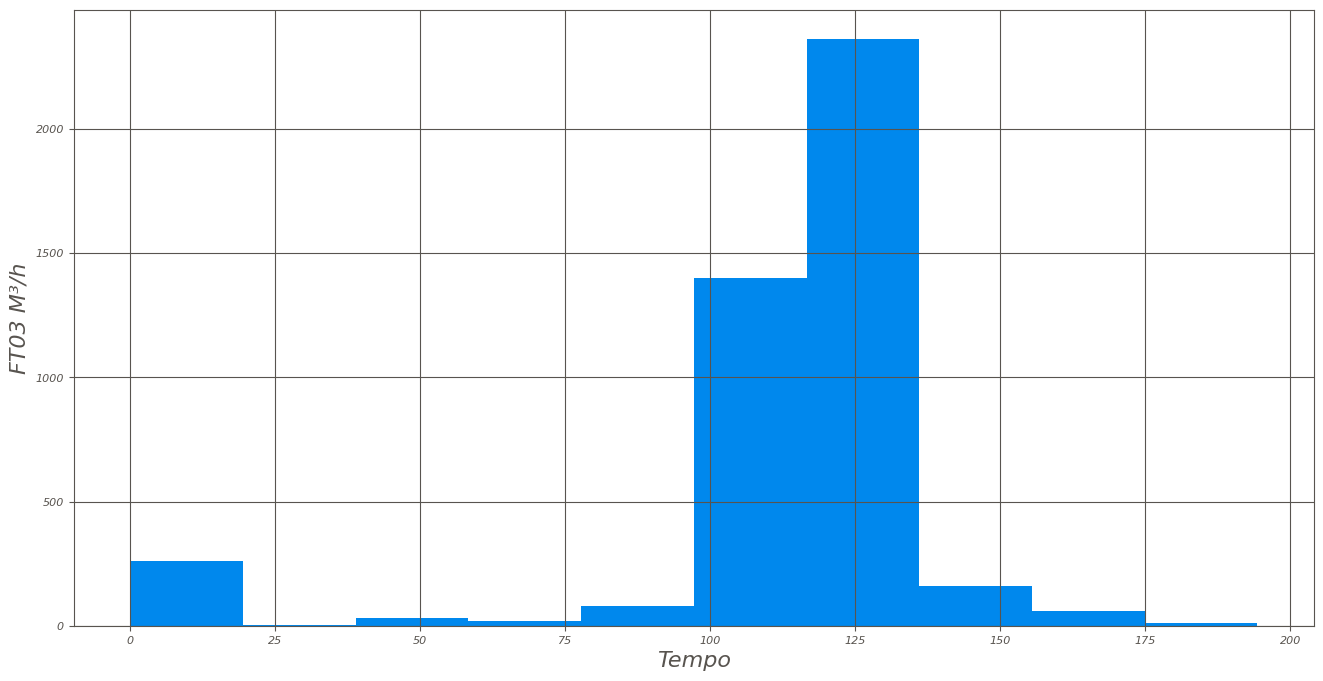
\includegraphics[width=0.9\linewidth]{Resultados/Figuras/ft03}
		
		\fonte{Elaboração própria a partir de dados da SANEPAR (2018 a 2020)}
	\end{figure}
	
Para responder à pergunta \ref{q5}\ref{q5:e}, a Figura \ref{fig:ft03} ilustra como a vazão pode ser afetada pelo nível do tanque. É interessante observar que a vazão de recalque tem um impacto mais significativo no nível do tanque em comparação com as outras vazões. Isso ocorre porque a vazão de recalque está associada à injeção de água diretamente no tanque por meio da bomba localizada próxima à base do tanque. Por outro lado, as demais vazões apresentam alguns valores ausentes, o que limita sua influência na análise geral.	
	


De acordo com o \citeonline{Reisen2017115}, o teste DF tem as seguintes equações

\begin{eqnarray}
	z_t&=& y_t+\theta \beta_t, \qquad t=1,\ldots, T, \label{eq:df3}\\	
	\hat{\rho}_{\mathrm{DF}}-1&=&\frac{\sum_{t=1}^T z_{t-1} \Delta z_t}{\sum_{t=1}^T z_{t-1}^2} \label{eq:regdf}
\end{eqnarray}

De \eqref{eq:regdf} onde $\Delta z_t=z_t-z_{t-1}$. Sob a hipótese nula $\left(H_0\right)$ : `` $\rho=1$'', as estatísticas do teste DF e suas distribuições limitantes são dadas da seguinte forma:


\begin{eqnarray}
	T\left(\hat{\rho}_{\mathrm{DF}}-1\right)=T \frac{\sum_{t=1}^T z_{t-1} \Delta z_t}{\sum_{t=1}^T z_{t-1}^2}
\end{eqnarray}
e


\begin{eqnarray}
	\hat{\tau}_{\mathrm{DF}}&=&\frac{\hat{\rho}_{\mathrm{DF}}-1}{\hat{\sigma}_{\mathrm{DF}}\left(\sum_{t=1}^T z_{t-1}^2\right)^{-1 / 2}} \label{eq:df}
\end{eqnarray}

De \eqref{eq:df} onde $\hat{\sigma}_{\mathrm{DF}}^2=T^{-1} \sum_{t=1}^T\left(\Delta z_t-\left(\hat{\rho}_{\mathrm{DF}}-1\right) z_{t-1}\right)^2 .$



Suponha que $\left(z_t\right)_{1 \leq t \leq T}$ são dadas por \eqref{eq:df3}, então quando $\rho=1$,


\begin{eqnarray}
	T\left(\hat{\rho}_{\mathrm{DF}}-1\right) \stackrel{d}{\longrightarrow} \frac{W(1)^2-1}{2 \int_0^1 W(r)^2 \mathrm{~d} r}-\left(\frac{\theta}{\sigma}\right)^2 \frac{\pi}{\int_0^1 W(r)^2 \mathrm{~d} r}, \text { como } T \rightarrow \infty \\
	\hat{\tau}_{\mathrm{DF}} \stackrel{d}{\longrightarrow}\left[1+2(\theta / \sigma)^2 \pi\right]^{-1 / 2}\left\{\frac{W(1)^2-1}{2\left(\int_0^1 W(r)^2 \mathrm{~d} r\right)^{1 / 2}}-\frac{(\theta / \sigma)^2 \pi}{\left(\int_0^1 W(r)^2 \mathrm{~d} r\right)^{1 / 2}}\right\} \\
	\quad \operatorname{como} T \rightarrow \infty\label{eq:df2}
\end{eqnarray}

A partir de \eqref{eq:df2}, onde $\stackrel{d}{\longrightarrow}$ denota convergência na distribuição e onde $\left\{W(r), r \in[0,1]\right\}$ denota o movimento Browniano padrão.

O ACF (do inglês \textit{Auto-Correlation Function}) é uma medida estatística utilizada para identificar a presença de correlação serial em uma série temporal. Ele calcula a autocorrelação entre os valores da série em diferentes defasagens, ou seja, a correlação entre os valores atuais e os valores passados da série. 

O ACF é útil para analisar a dependência temporal dos dados e identificar padrões de sazonalidade, tendência ou outros efeitos temporais. Através do ACF, é possível avaliar se a série exibe autocorrelação significativa em defasagens específicas, o que pode indicar a presença de não estacionariedade ou estrutura temporal que precisa ser considerada na análise ou modelagem da série temporal.

\begin{figure}[!htb]
	\centering
	\caption{Autocorrelação e Autocorrelação parcial}
	\label{fig:acf}
	
	
	\begin{subfigure}{0.9\textwidth}
		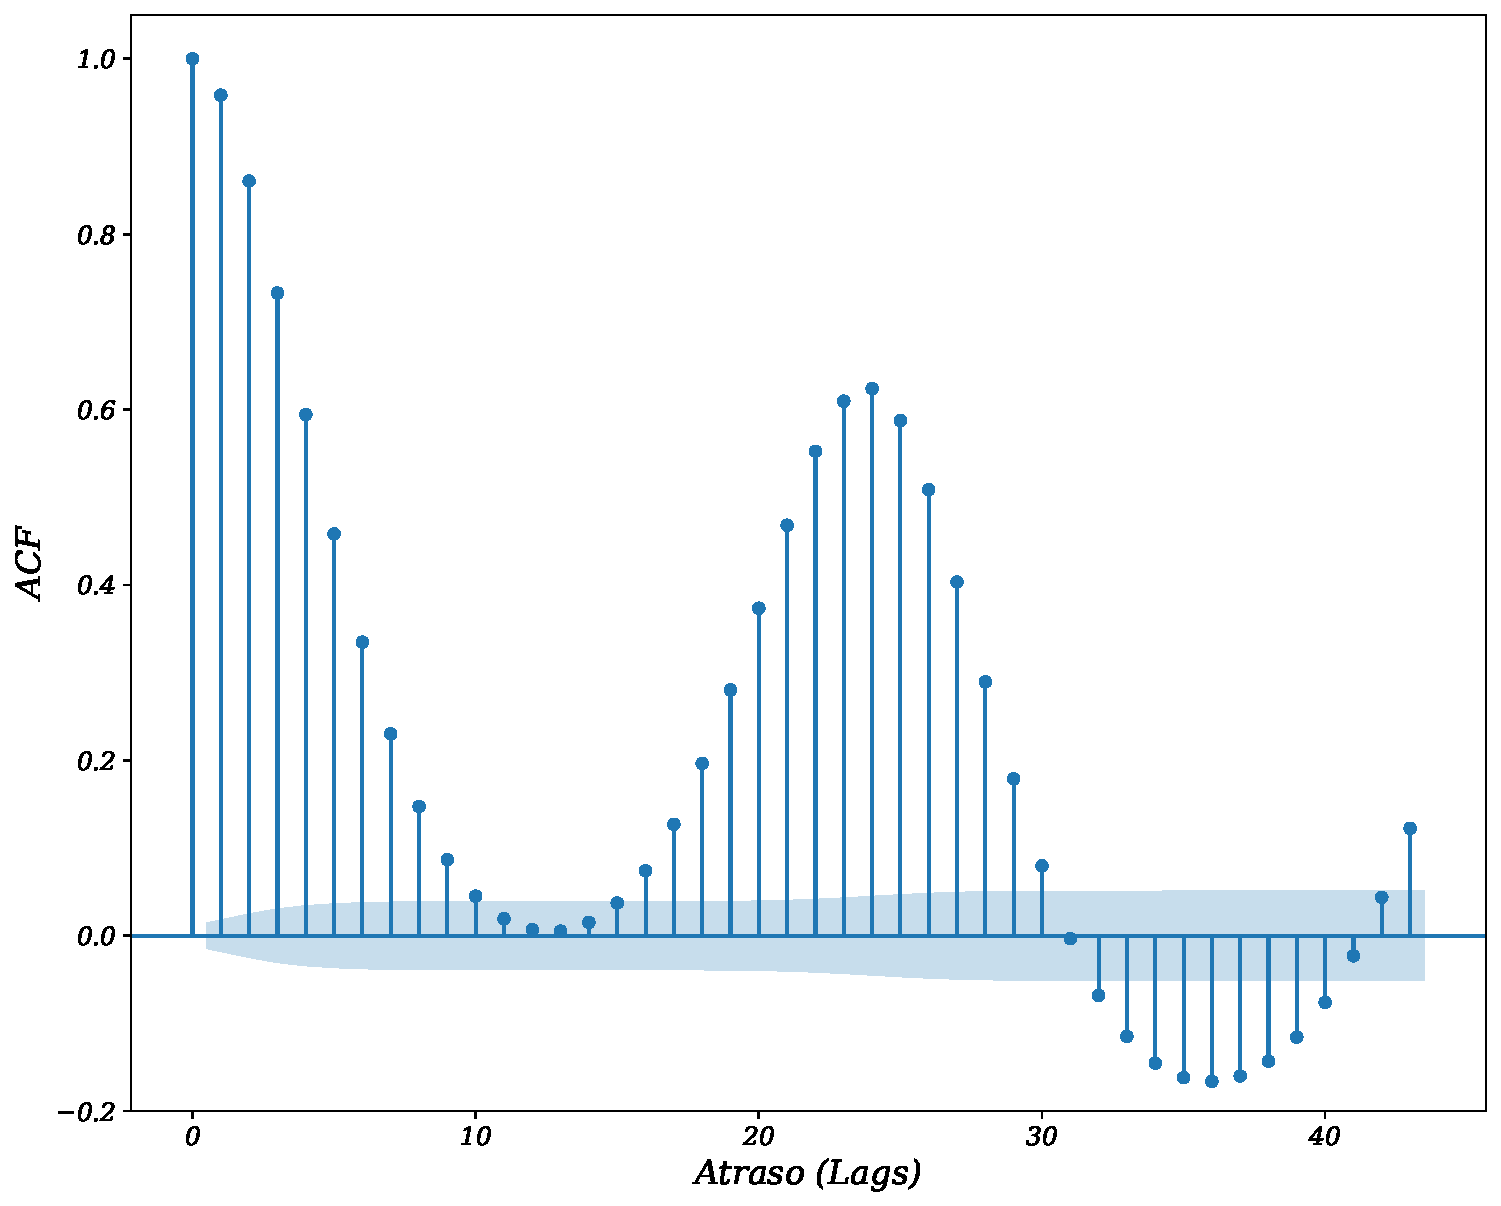
\includegraphics[width=\linewidth]{Resultados/Figuras/acf} 
		\caption{ACF}\label{fig:acfa}
	\end{subfigure}
	

	\begin{subfigure}{0.9\textwidth}
		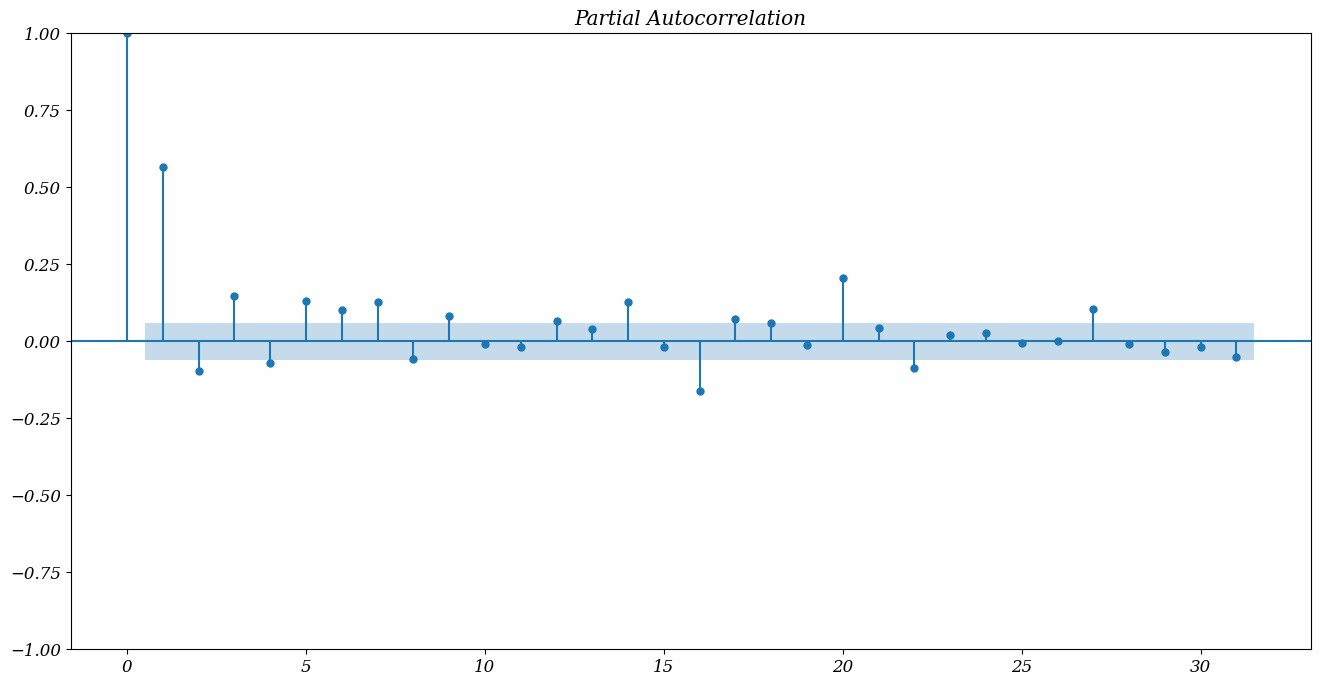
\includegraphics[width=\linewidth]{Resultados/Figuras/pacf}
		\caption{PACF}\label{fig:pacf}
	\end{subfigure}
	
	\fonte{Elaboração própria a partir de dados da SANEPAR (2018 a 2020)}
\end{figure}

A estatística ADF (do ingê \textit{Augmented Dickey-Fuller}) de $-4,27$ indica a evidência de estacionariedade na série temporal. Quanto mais negativo for o valor da estatística ADF, maior é a evidência de estacionariedade nos dados.

O valor-p de $0,0005$, por sua vez, está associado ao teste ADF. O valor-p é uma medida estatística que representa a probabilidade de obter um resultado igual ou mais extremo do que o observado, sob a suposição de que a hipótese nula seja verdadeira. No caso do teste ADF, a hipótese nula é a presença de raiz unitária na série temporal, o que indica não estacionariedade. Assim, um valor-p baixo (geralmente abaixo de um nível de significância predefinido, como 0,05) sugere que a série temporal é estacionária, enquanto um valor-p alto sugere que a série temporal é não estacionária. Neste caso, o valor-p de $0,0005$ é bastante baixo, o que indica forte evidência contra a hipótese nula e sugere que a série temporal é estacionária.

Na Figura \ref{fig:acf}, pode-se observar a diferença entre a autocorrelação (ACF) exibida na Figura \ref{fig:acfa} e a autocorrelação parcial (PACF) exibida na Figura \ref{fig:pacf}. A autocorrelação é uma medida da correlação entre os valores da série temporal em diferentes defasagens, levando em consideração tanto a correlação direta quanto a correlação indireta. Por outro lado, a autocorrelação parcial mede apenas a correlação direta entre os valores, desconsiderando a influência das defasagens intermediárias. Essas análises são úteis para identificar padrões e relações de dependência entre os valores da série temporal, fornecendo informações importantes para a modelagem e previsão desses dados.

O intervalo de confiança padrão de 95\% é representado pela marca azul na Figura. As observações que estão fora desse intervalo são consideradas estatisticamente correlacionadas, indicando a presença de padrões ou estrutura na série temporal.

A correlação visualizada na Figura \ref{fig:acf} é fundamental para a interpretação do teste DF. Em uma série de ruído branco, os valores são completamente aleatórios e não apresentam correlação significativa. Portanto, quando há correlação presente na série, isso indica a existência de padrões ou dependências entre os valores, o que pode ser explorado para a modelagem e previsão da série temporal.

\begin{figure}[!htb]
	\centering
	\caption{Ruído branco}
	\label{fig:ruido-branco}
	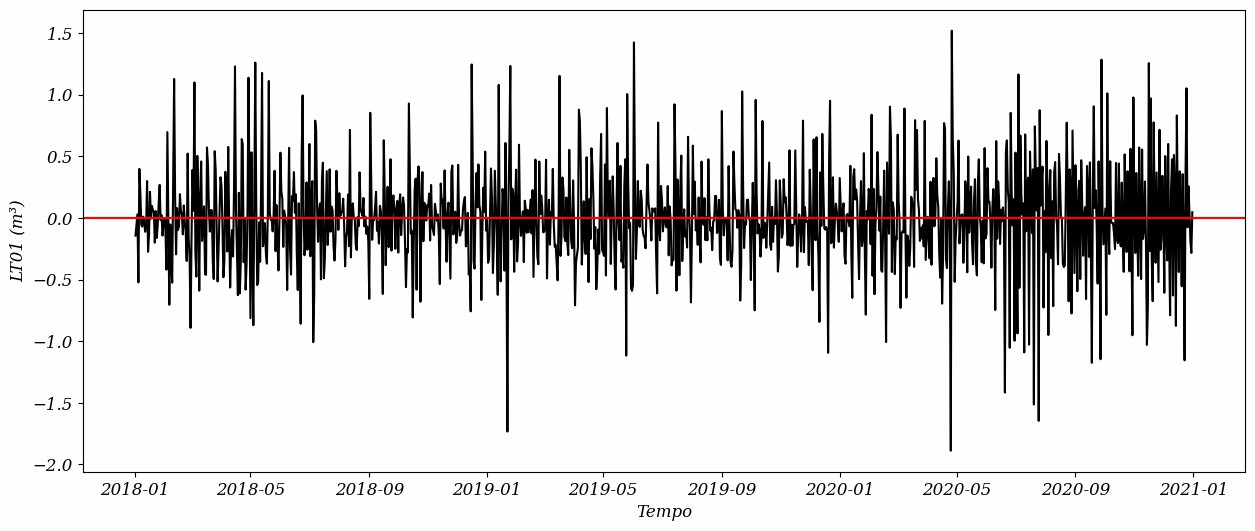
\includegraphics[width=0.9\linewidth]{Resultados/Figuras/ruido-branco}
	
	\fonte{Elaboração própria a partir de dados da SANEPAR (2018 a 2020)}
\end{figure}

Na Figura \ref{fig:ruido-branco}, é possível observar uma série temporal que pode ser caracterizada como ruído branco. Uma série temporal é considerada ruído branco se suas variáveis forem independentes e distribuídas de forma idêntica, com média zero. Isso implica que todas as variáveis possuem a mesma variância ($\sigma^2$) e que cada valor não possui correlação com os demais valores da série.

Além disso, é importante destacar o comprimento dos zeros na variável prevista, o que conclui a etapa \ref{etp:3}.

\subsubsection{Separa\c c\~ao dos dados}\label{subsubsec:divisao}

Na etapa \ref{etp:4}, os dados foram divididos em conjuntos de treinamento, teste e validação. Essa prática é comum entre profissionais de aprendizado de máquina, pois permite avaliar o desempenho do modelo em conjuntos de dados diferentes.

Em relação ao processamento de modelos de aprendizado profundo, é importante mencionar as inovações trazidas pela empresa Nvidia ao longo dos anos, especialmente no campo do processamento de imagens. O lançamento da placa de vídeo GeForce RTX 4090 tem sido bastante aguardado tanto por gamers quanto por profissionais que lidam com aprendizado de máquina.

No contexto do estudo, foram utilizados dois computadores para realizar os cálculos dos modelos. Um deles é equipado com um processador Intel Core i5-3330 e o outro é um notebook com um processador Intel Core i7-5500. Ambos os processadores possuem 4 threads, sendo que o notebook possui 2 núcleos físicos e o i5 possui 4 núcleos físicos. Cada processador tem suas especificações e desempenho adequados a diferentes necessidades. Vale ressaltar que não é obrigatório utilizar as últimas gerações de processadores para realizar esses processamentos, e sim compreender e aplicar corretamente os recursos disponíveis.

Quanto à divisão dos dados, foi adotada uma estratégia básica em que 70\% dos dados foram destinados ao conjunto de treinamento e os 30\% restantes foram reservados para o conjunto de teste. Dentro dos 70\% de treinamento, foi realizada uma subdivisão em que 80\% desses dados foram usados novamente para treinamento e os 20\% restantes foram utilizados para validação. Essa abordagem foi implementada em linguagem de programação para facilitar o processo e evitar a necessidade de recalculá-la a cada modificação do modelo.

\subsubsection{Estrat\'egia de Previs\~ao}\label{subsubsec:est}

A estratégia recursiva é mencionada por \citeonline{PETROPOULOS2022705} como uma abordagem eficaz na previsão de séries temporais de múltiplos passos. De acordo com o autor, essa estratégia envolve o uso de previsões anteriores como entradas para prever os próximos passos da série temporal. A abordagem recursiva tem demonstrado potencial para melhorar a acurácia das previsões de séries temporais de longo prazo.

Na Etapa \ref{etp:5}, discute-se a previsão dos dados em uma janela de horizonte de previsão estendida, abrangendo diferentes períodos de tempo, como um dia, uma semana, duas semanas e um mês. Essa estratégia de previsão recorrente permite a comparação entre modelos de regressão e modelos ARIMA em diferentes horizontes temporais.

Essa abordagem é vantajosa, pois cada modelo possui suas próprias características e desempenho ao lidar com previsões de curto prazo, como um dia, e previsões de prazo mais longo, como um mês. Ao utilizar uma janela de previsão mais ampla, é possível observar e avaliar melhor as diferenças entre os modelos e analisar seu desempenho em horizontes de tempo variados.

\textbf{Validação e ajuste do modelo}
na etapa \ref{etp:6}, o horizonte de previsão foi personalizado com base no método recursivo de previsão de série temporal e na previsão do nível do tanque LT01. Foram selecionados os seguintes passos para a previsão à frente: uma hora, seis horas, doze horas e um dia. Essa escolha do horizonte de previsão foi feita levando em consideração a estratégia recursiva e os objetivos específicos do estudo. Identifica-se que essa janela de tempo proporciona uma análise mais adequada e comparável entre os modelos utilizados.

Foram utilizados os parâmetros obtidos pelo autoARIMA, que são $(p = 7, d = 0, q = 0) (P = 2, D = 1, Q = 1)_{M = 12}$, mas foram ajustados para obter um melhor resultado, sendo $(p = 7, d = 1, q = 7) (P = 2, D = 1, Q = 1)_{M = 12}$. Na Tabela \ref{tab:autoarima_params}, são exibidos todos os modelos obtidos por esse método do ``autoARIMA'' e ajustados para que obtenham o melhor resultado.
\(p\): Ordem do componente AR (\textit{Auto-Regressivo}),
\(d\): Número de diferenciações não sazonais,
\(q\): Ordem do componente MA (\textit{Média Móvel}),
\(P\): Ordem do componente AR sazonal,
\(D\): Número de diferenciações sazonais,
\(Q\): Ordem do componente MA sazonal,
\(M\): Período sazonal (número de observações em um ciclo sazonal).
Na Tabela \ref{tb:resltsar} mostra como a biblioteca do Python autoARIMA obteve os resultados dos parâmetros, exibindo o STD e os intervalos de confiança nos quais o modelo alcançou o melhor desempenho. O leve ajuste realizado não altera significativamente os parâmetros obtidos nesta biblioteca, permitindo que cada modelo seja trabalhado de maneira eficiente.

\begin{table}[!htb]
	\centering
	\caption{Parâmetros utilizados nos modelos ARIMA e seus antecessores obtidos pelo ``autoARIMA'' do Python.}
	\label{tab:autoarima_params}
	\small
	\begin{tabular}{
			>{\centering\arraybackslash}p{5.5cm}
			>{\centering\arraybackslash}p{6cm}
			>{\centering\arraybackslash}p{3cm}
		}
		\toprule
		\textbf{Modelo} & \textbf{Parâmetros Utilizados} & \textbf{Método de Estimação} \\
		\midrule
		AR(p) & \( p = 7 \) & AutoARIMA \\
		ARX(p) & \( p = 7 \) & AutoARIMA \\
		MA(q) & \( q = 7 \) & AutoARIMA  \\
		ARMA(p, q) & \( p = 7 \), \( q = 7 \) & AutoARIMA  \\
		ARIMA(p, d, q) & \( p = 7 \), \( d = 1 \), \( q = 7 \) & AutoARIMA  \\
		ARIMAX(p, d, q) & \( p = 7 \), \( d = 1 \), \( q = 7 \) & AutoARIMA  \\
		SARIMA(p, d, q)(P, D, Q) & \( p = 7 \), \( d = 1 \), \( q = 7 \), \( P = 2 \), \( D = 1 \), \( Q = 1 \), \( M = 12 \) & AutoARIMA  \\
		SARIMAX(p, d, q)(P, D, Q, M) & \( p = 7 \), \( d = 1 \), \( q = 7 \), \( P = 2 \), \( D = 1 \), \( Q = 1 \), \( M = 12 \) & AutoARIMA  \\
		\bottomrule
	\end{tabular}
\end{table}



\begin{table}[!htb]
	\centering
	\caption{SARIMAX$(7, 0, 0)\times(2, 1, [1], 12)$ Results} \label{tb:resltsar}
	\begin{tabular}{
			l
			S[table-format=1.4]
			S[table-format=1.4]
			S[table-format=3.3]
			S[table-format=1.3]
			S[table-format=1.3]
			S[table-format=1.3]
		}
		\toprule
		& {Coef} & {STD Err} & {z} & {P$>|z|$} & {[0,025} & {0,975]} \\
		\midrule
		Intercept & 0,0003 & 0,000 & 1,053 & 0,292 & -0,000 & 0,001 \\
		ar.L1 & 1,6149 & 0,011 & 141,865 & 0,000 & 1,593 & 1,637 \\
		ar.L2 & -0,8879 & 0,021 & -42,045 & 0,000 & -0,929 & -0,847 \\
		ar.L3 & 0,3167 & 0,024 & 13,033 & 0,000 & 0,269 & 0,364 \\
		ar.L4 & -0,1056 & 0,027 & -3,961 & 0,000 & -0,158 & -0,053 \\
		ar.L5 & -0,1099 & 0,028 & -3,928 & 0,000 & -0,165 & -0,055 \\
		ar.L6 & 0,1431 & 0,027 & 5,368 & 0,000 & 0,091 & 0,195 \\
		ar.L7 & -0,0673 & 0,015 & -4,583 & 0,000 & -0,096 & -0,039 \\
		ar.S.L12 & -0,1222 & 0,016 & -7,705 & 0,000 & -0,153 & -0,091 \\
		ar.S.L24 & 0,1692 & 0,014 & 12,244 & 0,000 & 0,142 & 0,196 \\
		ma.S.L12 & -0,8728 & 0,012 & -74,569 & 0,000 & -0,896 & -0,850 \\
		sigma2 & 0,0157 & 0,000 & 60,022 & 0,000 & 0,015 & 0,016 \\
		\bottomrule
	\end{tabular}
\end{table}


Para os modelos de gradiente \textit{boosting} e redes neurais artificiais, os hiperparâmetros foram otimizados usando a biblioteca Optuna do Python. Nesse contexto, são empregadas técnicas bayesianas, especificamente o algoritmo TPE, visando uma otimização mais eficiente.

Os modelos XGBoost e LightGBM tem como parâmetros e hiperparâmetros mostrado na Tabela \ref{tab:hiperparametros} a otimização dos paramétrios dos modelos XGBoost, LightGBM, RFR e DTR. Esses modelos, devido à sua semelhança, exibem tempos de desempenho próximos um do outro. 



\begin{table}[!htb]
	\centering
	\caption{Hiperparâmetros dos modelos}
	\label{tab:hiperparametros}
	\begin{tabular}{
			>{\centering\arraybackslash}p{2.2cm}
			>{\centering\arraybackslash}p{2.8cm}
			>{\centering\arraybackslash}p{1.9cm}
			>{\centering\arraybackslash}p{1.9cm}
			>{\centering\arraybackslash}p{1.9cm}
			>{\centering\arraybackslash}p{1.9cm}
			>{\centering\arraybackslash}p{1.9cm}
		}
		\toprule
		\textbf{Modelo} & \textbf{Estimadores} & \textbf{Profund. Máxima} & \textbf{Min. Amostras Divisão} & \textbf{Min. Amostras por Folha} & \textbf{Máx. Recursos} & \textbf{Taxa de Aprendizado} \\
		\midrule
		XGB Regressor & 503 & 5 & 7 & 2 & ``sqrt'' & 0,034 \\
		LGBM Regressor & 820 & 10 & 3 & 5 & ``auto'' & 0,014 \\
		Random Forest Regressor & 135 & 10 & 4 & 2 & None & N/A \\
		Decision Tree Regressor & N/A & 229 & 32 & 20 & None & N/A \\
		\bottomrule
	\end{tabular}
\end{table}



Os modelos de rede neural artificial, como RNN, ANN, CNN, GRU, LSTM e Transformer, obtidos na otimização do Optuna do Python, tiveram seus hiperparâmetros melhorados, conforme exibido na Tabela \ref{tab:hyperparameters_summary}. Esses modelos, por serem modelos de rede neural artificial, são melhores para otimizar do que os outros. 

\begin{table}[!htb]
	\centering
	\caption{Resumo dos Hiperparâmetros dos Modelos de Redes Neurais}
	\label{tab:hyperparameters_summary}
	\small
	\begin{tabular}{
			>{\centering\arraybackslash}p{1.8cm}
			>{\centering\arraybackslash}p{2cm}
			>{\centering\arraybackslash}p{2cm}
			>{\centering\arraybackslash}p{2cm}
			>{\centering\arraybackslash}p{2cm}
			>{\centering\arraybackslash}p{1.5cm}
			>{\centering\arraybackslash}p{2.5cm}
		}
		\toprule
		\textbf{Modelo} & \textbf{Unidades/ Layers} & \textbf{Heads/ Dimensões} & \textbf{Tamanho do Batch} & \textbf{Épocas} & \textbf{Dropout/ Learning Rate} & \textbf{Outros Parâmetros} \\
		\midrule
		LSTM & 128 & -- & 32 & 77 & -- & -- \\
		
		GRU & -- & -- & 32 & 50 & -- & -- \\
		
		Transformers & -- & 8 heads, 217; 433 & -- & 50 & -- & 2 camadas \\
		
		RNN & 79 & -- & 16 & 50 & 0,0008612 & -- \\
		
		CNN & -- & -- & 61 & 10 & 0,2799; 0,00052 & Kernel: 7, Densas: 1, Verbosidade: 1 \\
		
		ANN & 125 & -- & 27 & 96 & 0,4135, 0,0004057 & Densas: 1, Verbosidade: 0 \\
		\bottomrule
	\end{tabular}
\end{table}



\subsubsection{Modelos de previs\~ao e m\'etricas de desempenho}\label{subsubsec:modelos}

A partir da etapa \ref{etp:7}, foram utilizadas três métricas amplamente empregadas na literatura para a previsão e comparação de modelos ARIMA e modelos de regressão. Essas métricas foram detalhadas na seção \ref{subsec:metrica}.

Ao analisar os modelos desenvolvidos, foi observado que o modelo de regressão linear (LR) obteve o melhor desempenho tanto na previsão de curto prazo, considerando uma modelagem de 24 horas, quanto nas horas de pico entre 18h e 21h. Os modelos MA, AR, SARIMA, ARIMA, SARIMAX, ARIMAX, ARX, LGBMRegressor, XGBRegressor e RFR também apresentaram um desempenho satisfatório, seguindo uma ordem de melhor para pior.

Para previsões de longo prazo, como no caso dos 30 dias, foram avaliados os modelos ARMA, AR, MA, ARIMA, ARIMAX, ARX, SARIMA, SARIMA, XGBRegressor, RFR, LGBMRegressor e LR, novamente seguindo a ordem de melhor desempenho. No entanto, ao analisar os resultados graficamente nos apêndices, foi observado que os modelos que incorporam variáveis exógenas parecem ter uma capacidade de previsão superior em relação aos demais modelos. Essa tendência pode ser visualizada nas Figuras de \ref{fig:1-AR-ARX-MA24} a \ref{fig:60-ARIMAX-SARIMA-SARIMAX24} e nas Tabelas de \ref{tb:1-24trn} a \ref{tb:60-24cm}.


\subsubsection{Relat\'orio dos Resultados}

Na etapa \ref{etp:9}, foi utilizado o teste de Friedman e Nemenyi para comparar as classificações médias entre os classificadores. O teste de Nemenyi é um teste de comparação múltipla utilizado após a aplicação de testes não paramétricos com três ou mais fatores.

\begin{table}[!htb]
	\centering
	\caption{Teste Nemenyi}
	\begin{tabular}{@{}clllllllll@{}}
		\toprule
		\multicolumn{1}{l}{\textbf{Nemenyi}} & \multicolumn{1}{c}{\textbf{0}} & \multicolumn{1}{c}{\textbf{1}} & \multicolumn{1}{c}{\textbf{2}} & \multicolumn{1}{c}{\textbf{3}} & \multicolumn{1}{c}{\textbf{4}} & \multicolumn{1}{c}{\textbf{5}} & \multicolumn{1}{c}{\textbf{6}} & \multicolumn{1}{c}{\textbf{7}} & \multicolumn{1}{c}{\textbf{8}} \\ \midrule
		\textbf{0}                           & 1,000                          & 0,001                          & 0,001                          & 0,001                          & 0,001                          & 0,001                          & 0,001                          & 0,001                          & 0,001                          \\
		\textbf{1}                           & 0,001                          & 1,000                          & 0,001                          & 0,001                          & 0,001                          & 0,001                          & 0,001                          & 0,001                          & 0,157                          \\
		\textbf{2}                           & 0,001                          & 0,001                          & 1,000                          & 0,847                          & 0,001                          & 0,001                          & 0,001                          & 0,001                          & 0,001                          \\
		\textbf{3}                           & 0,001                          & 0,001                          & 0,847                          & 1,000                          & 0,001                          & 0,001                          & 0,001                          & 0,001                          & 0,001                          \\
		\textbf{4}                           & 0,001                          & 0,001                          & 0,001                          & 0,001                          & 1,000                          & 0,001                          & 0,001                          & 0,001                          & 0,001                          \\
		\textbf{5}                           & 0,001                          & 0,001                          & 0,001                          & 0,001                          & 0,001                          & 1,000                          & 0,001                          & 0,001                          & 0,001                          \\
		\textbf{6}                           & 0,001                          & 0,001                          & 0,001                          & 0,001                          & 0,001                          & 0,001                          & 1,000                          & 0,001                          & 0,001                          \\
		\textbf{7}                           & 0,001                          & 0,001                          & 0,001                          & 0,001                          & 0,001                          & 0,001                          & 0,001                          & 1,000                          & 0,001                          \\
		\textbf{8}                           & 0,001                          & 0,157                          & 0,001                          & 0,001                          & 0,001                          & 0,001                          & 0,001                          & 0,001                          & 1,000                          \\ \bottomrule
	\end{tabular}
	
	\fonte{Elaboração própria a partir de dados da SANEPAR (2018 a 2020)}
\end{table}

Para calcular a estatística de teste $F_r$ de Friedman, inicialmente cria-se uma tabela com os dados, onde cada linha representa uma amostra e cada coluna representa uma condição de teste. Em seguida, as amostras são ordenadas ao longo das condições, da melhor situação para a pior. Se não houver empates, a estatística de teste $F_r$ é calculada utilizando a seguinte fórmula:

\begin{equation}
	F_r = \left(\frac{12}{n k(k+1)} \sum_{i=1}^k R_i^2\right) - 3n(k+1)
\end{equation}

Nessa fórmula, $n$ é o número de linhas (ou amostras), $k$ é o número de colunas (ou condições) e $R_i$ é a soma das fileiras da coluna (ou condição) $i$.

Além disso, o valor crítico CD (Critical Difference) é utilizado para determinar se dois classificadores são significativamente diferentes um do outro. O CD é calculado usando a fórmula que mencionei anteriormente:

\begin{equation}
	CD = q_\alpha \sqrt{\frac{k(k+1)}{6N}}
\end{equation}

Na fórmula do CD, $q_\alpha$ é o valor crítico obtido da tabela de teste de Nemenyi, $k$ é o número de classificadores e $N$ é o número total de amostras.

De acordo com essa equação, os resultados da pesquisa foram os seguintes:

$statistic=8015.611,\ \ p-value=0.0$ com um total de 26.306 linhas por 9 colunas.


\subsubsection{Compara\c c\~ao dos Modelos}

Com o objetivo de obter uma análise mais aprofundada do desempenho de cada modelo, foi realizada uma comparação por meio de um gráfico de violino. Dessa forma, pôde-se observar qual dos modelos apresentava o melhor desempenho.



Ao examinar os modelos representados nas Figuras \ref{fig:modelos-arima} e \ref{fig:violin-lr-xgb-lgbm-rf}, identifico os modelos que se destacam em relação à natureza dos dados. Na Figura \ref{fig:basic_comparar}, que compara os modelos ARIMA e XGBoost com outros, torna-se evidente que os modelos ARIMA como AR, ARX, MA, ARMA, ARIMAX e SARIMAX demonstram um desempenho sólido. Além disso, os modelos baseados em gradientes e regressão, como o XGBoost, exibem resultados comparáveis, beneficiando-se da otimização por meio do Optuna, uma abordagem mais eficaz em relação aos tradicionais Grid Search e Randomized Search.

Na Figura \ref{fig:rrmse_comparar}, que contrasta as redes neurais com o modelo Prophet, é importante destacar que os modelos de redes neurais, incluindo RNN, LSTM, GRU, ANN, CNN e Transformer, foram avaliados em conjunto com o modelo Prophet. A análise estatística também demonstrou que o modelo RNN se sobressai como o vencedor entre as métricas avaliadas. Essa conclusão é respaldada pelas evidências de que pelo menos um modelo é superior aos demais. Os modelos com valores de p-valor abaixo de 0,05 foram realçados em \textit{itálico} para enfatizar sua significância.

A avaliação da eficácia dos modelos ARIMA em previsões de longo prazo emprega o teste de Ljung-Box, conforme detalhado no Apêndice \ref{sec:comtb18}. As Tabelas \ref{tb:lbtrn} a \ref{tb:lbcm} ilustram a acurácia dos modelos ARIMA ao longo do tempo, com valores menores sendo destacados em \textbf{negrito} e \textit{itálico} para facilitar a interpretação. Modelos como ARX, ARIMAX e SARIMAX, que incorporam variáveis exógenas, demonstram um desempenho superior nesse contexto. Esses modelos não lineares apresentam uma capacidade de previsão robusta em horizontes temporais mais longos, diferenciando-se positivamente dos outros modelos ARIMA. Na Figura \ref{fig:modelos-arima}, são selecionados os modelos ARIMA e seus antecessores. Esses modelos têm suas limitações, tanto para horizontes de previsão de curto prazo quanto para horizontes de longo prazo. Nessa comparação no gráfico de violino, são combinados vários outros gráficos em um só, como o gráfico de barras e o boxplot. Esse gráfico pode fornecer várias informações, mas o objetivo aqui é identificar apenas o melhor modelo entre os modelos ARIMA.
Como essa série não apresentou uma estacionariedade bem definida e os dados não a tornaram estacionária, os modelos que não têm sazonalidade mostraram-se superiores, tais como AR, MA, ARX, ARMA, ARIMA e ARIMAX. O modelo ARIMAX demonstrou ser bastante robusto para este caso, mas mesmo assim, modelos mais básicos como AR e MA ainda apresentaram resultados melhores.

\begin{figure}[H]
	\centering
	\caption{Comparação dos modelos ARIMA}\label{fig:modelos-arima}
	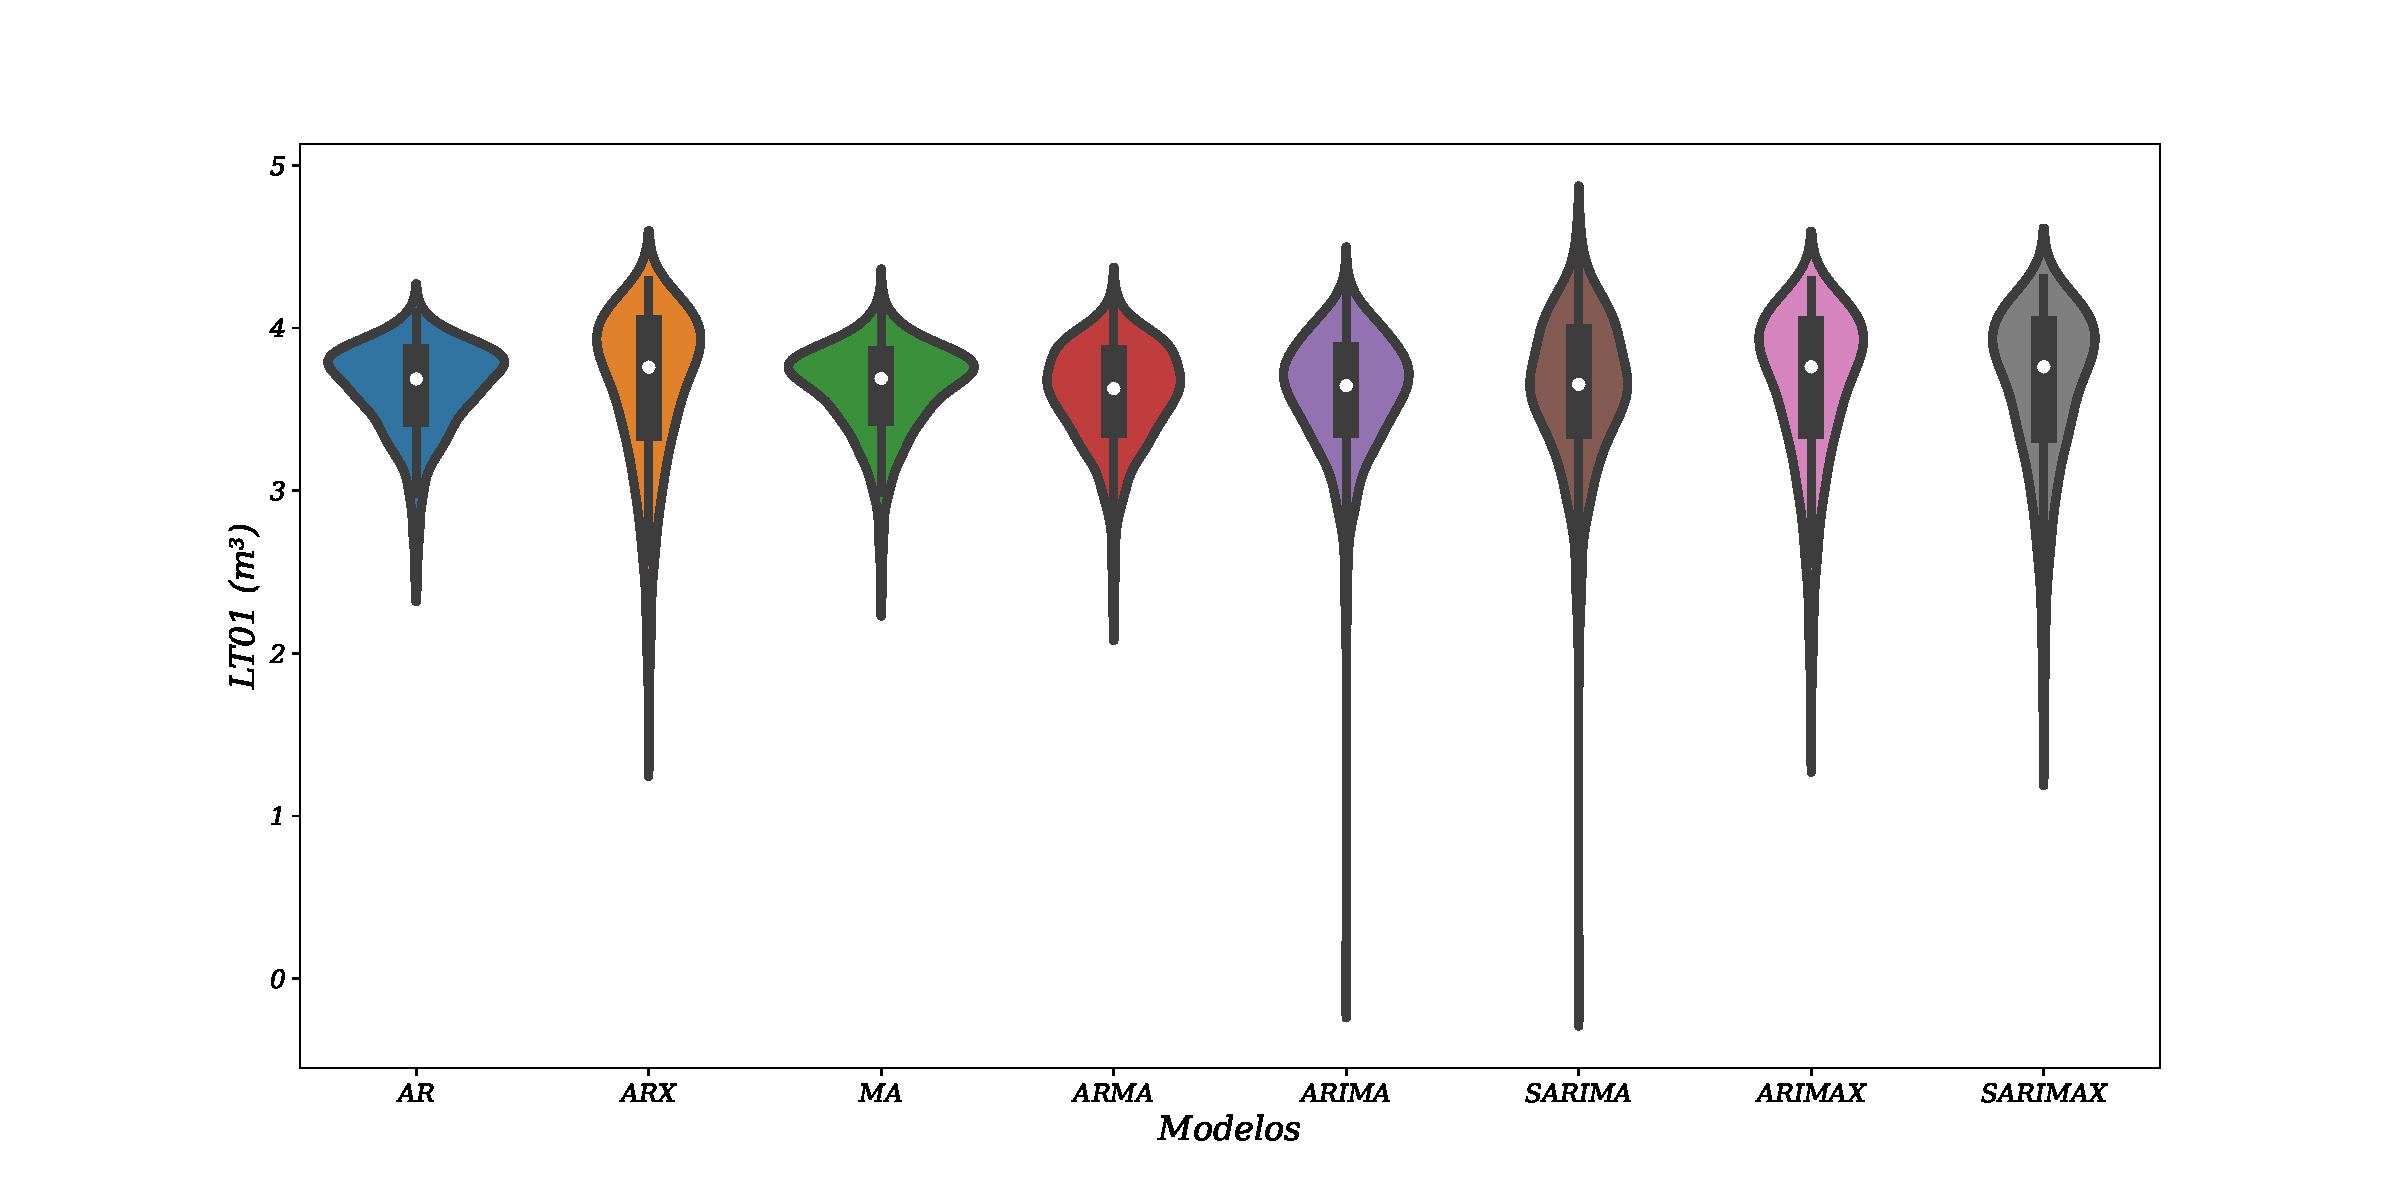
\includegraphics[width=1\linewidth]{Resultados/Figuras/modelos-arima}
	

\end{figure}

Na Figura \ref{fig:violin-lr-xgb-lgbm-rf}, é feita uma comparação entre os modelos de gradiente e regressor. Esses modelos, por serem mais robustos e utilizar técnicas de otimização mais avançadas, mostram-se superiores aos modelos comparados. O modelo XGBoost, em particular, é identificado como superior em relação aos outros modelos na análise.

\begin{figure}[H]
	\centering
	\caption{Comparação de modelos de regressão}\label{fig:violin-lr-xgb-lgbm-rf}
	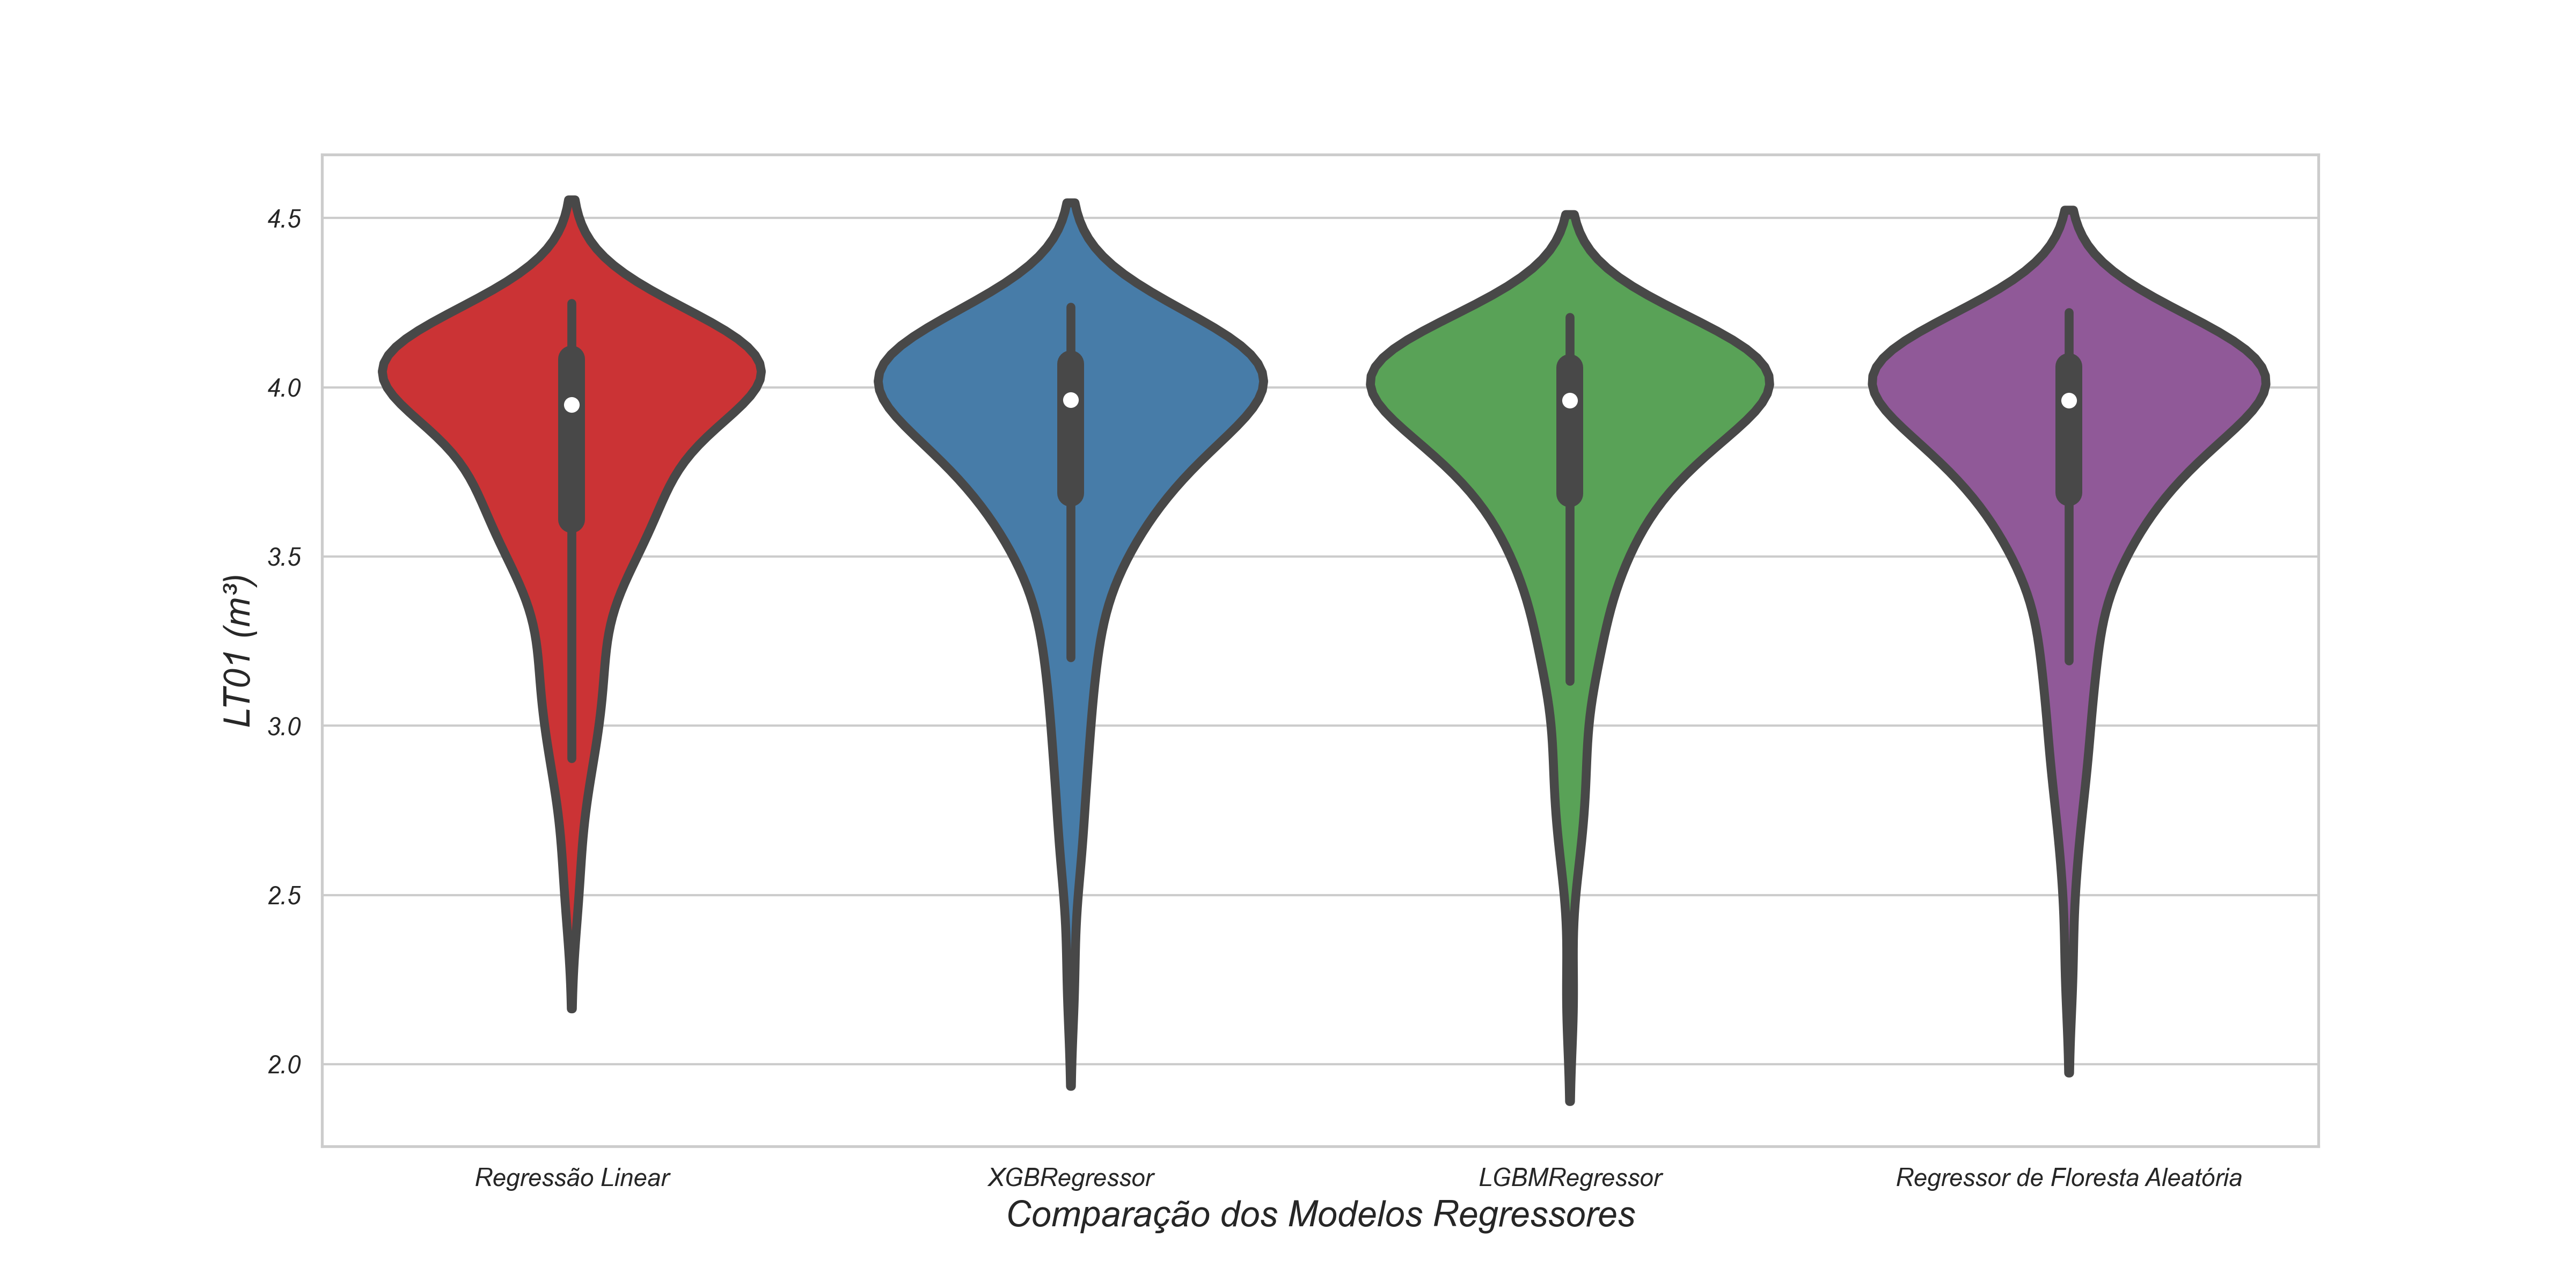
\includegraphics[width=1\linewidth]{Resultados/Figuras/violin-LR-XGB-LGBM-RF}
	
\end{figure}


Na Figura \ref{fig:rrmse_comparar}, nota-se que todos os modelos trabalhados aqui, exceto o modelo LR, foram comparados em relação às métricas de desempenho. Mesmo sendo muito robustos, esses modelos não conseguiram obter um resultado tão bom quanto o RNN.

\begin{figure}[H]
	\centering
	\caption{Análise comparativa dos modelos utilizando gráfico de barras \label{fig:rrmse_comparar} \label{fig:basic_comparar}}
	\begin{subfigure}{1\textwidth}
		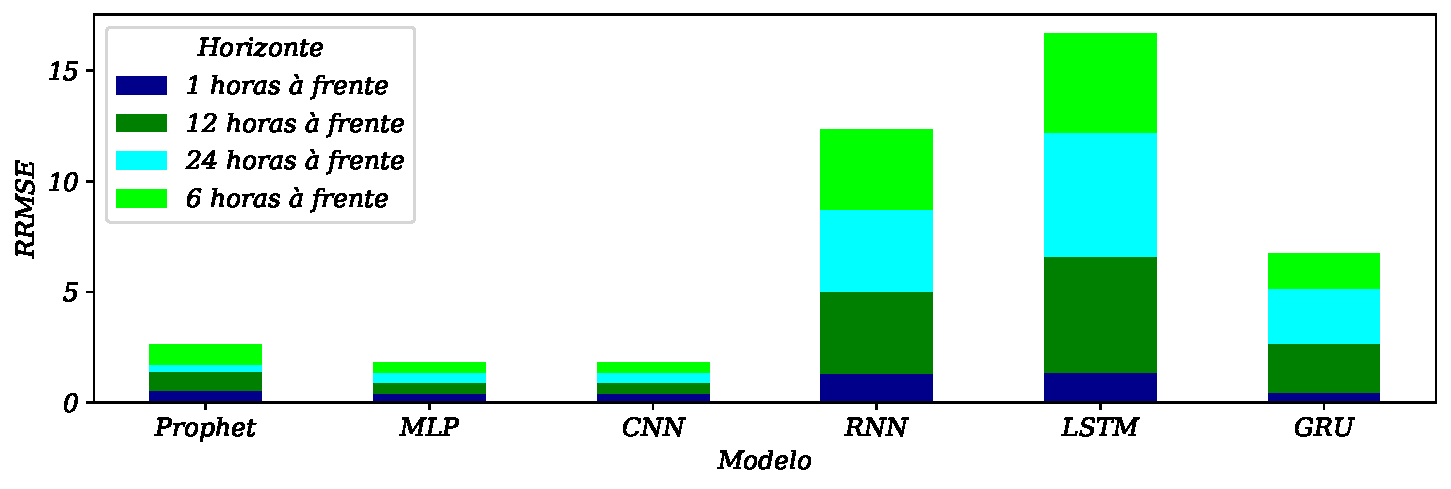
\includegraphics[width=\linewidth]{Resultados/Figuras/rrmse_comparar}
	
		
	\end{subfigure}
	
	\begin{subfigure}{1\textwidth}
		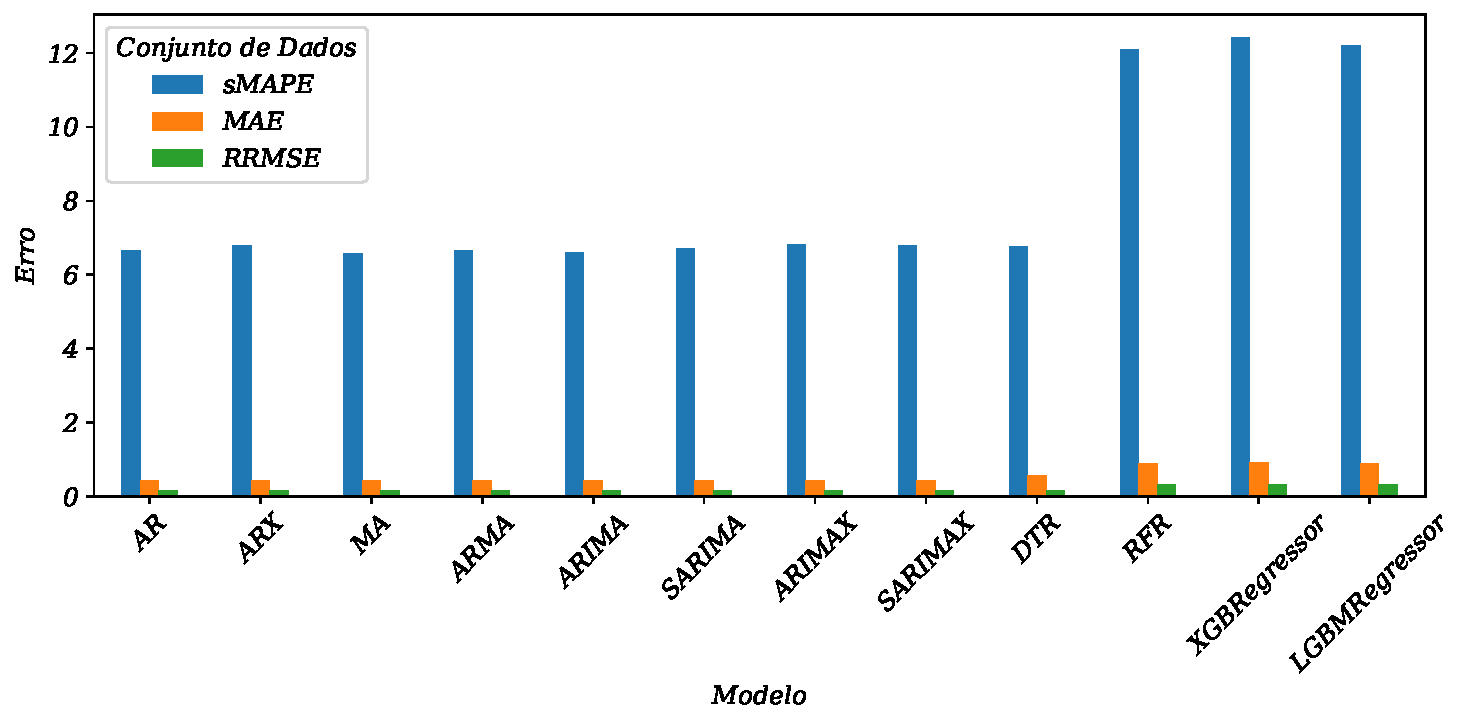
\includegraphics[width=\linewidth]{Resultados/Figuras/basic_comparar}
		
		
	\end{subfigure}
	

\end{figure}

  

\subsection{Aplica\c c\~ao do Mundo Real}\label{subsec:estudo-reslt}


A previsão da demanda de água é uma preocupação fundamental para muitas organizações e autoridades responsáveis pelo abastecimento de água. Neste estudo de caso, explorou-se como a análise de séries temporais pode ser aplicada para prever a demanda de água ao longo do tempo.

A análise de séries temporais é uma abordagem comumente utilizada para prever padrões futuros com base em dados históricos. No estudo, foram aplicadas técnicas de modelagem e previsão, permitindo obter valiosos sobre a demanda de água futura. Diversos modelos, como ARIMA e SARIMA, foram empregados para analisar os dados históricos e gerar previsões confiáveis.
Ao longo do estudo, identificaram-se sazonalidades na demanda de água, bem como padrões de consumo que variam ao longo do tempo. Essas informações são essenciais para o planejamento adequado do abastecimento de água, permitindo uma alocação eficiente dos recursos e uma resposta adequada às flutuações de demanda.

A aplicação da análise de séries temporais na previsão da demanda de água proporciona uma base sólida para a tomada de decisões informadas. Com base nos resultados obtidos, é possível ajustar estratégias de gerenciamento, antecipar picos de demanda e otimizar o uso dos recursos hídricos disponíveis.
Em suma, este estudo demonstrou que a análise de séries temporais é uma abordagem eficaz para prever a demanda de água ao longo do tempo. Ao fornecer precisos e confiáveis, essa técnica contribui para o planejamento e o gerenciamento eficiente do abastecimento de água, promovendo a sustentabilidade e a utilização racional dos recursos hídricos.



\subsubsection{Descri\c c\~ao do Sistema de Abastecimento de \'Agua}



Foram realizadas análises e modelagens utilizando a abordagem de séries temporais para prever a demanda diária de água em uma determinada cidade para os próximos seis meses. Os resultados obtidos forneceram valiosos sobre a demanda futura e contribuíram para um melhor planejamento do abastecimento hídrico. A seguir, apresentam-se as principais conclusões para cada uma das perguntas de pesquisa:

\noindent\ref{q1}: Qual é a adequação da pressão atual para atender à demanda diária?

Após análise dos dados e das métricas utilizadas, conclui-se que a pressão atual é adequada para atender à demanda diária. Durante o período analisado, não foram identificadas situações de pressão insuficiente que afetassem o fornecimento de água.

\noindent\ref{q2}: Qual é o volume mínimo de água necessário no reservatório para evitar o acionamento das bombas durante o horário de pico?

Com base na frequência de funcionamento das bombas e na demanda durante o horário de pico, determinou-se que é necessário manter um volume mínimo de água no reservatório, correspondente a $5285,90$ litros, para evitar o acionamento das bombas nesse período.

\noindent\ref{q3}: Qual é a vazão ótima para atender à demanda diária?

Após análise e modelagem dos dados, identificou-se que a vazão ótima para atender à demanda varia conforme o período do dia e as características sazonais. A pressão necessária para atender à demanda é de $3,60$ PSI (do inglês \textit{pound-force per square inch}) na sucção.

\noindent\ref{q4}: Como encontrar o ponto de equilíbrio entre a demanda e a vazão?

Após análise e modelagem dos dados, foi constatado que não existe um ponto de equilíbrio entre a demanda e a vazão no reservatório. No entanto, identificou-se um volume mínimo de reserva de $3.545$ litros que permite manter um armazenamento adequado no reservatório sem a necessidade de acionar as bombas durante o período de maior custo energético.

Embora essa estimativa de volume mínimo seja importante para garantir o abastecimento contínuo durante o período de pico, é importante ressaltar que não há um equilíbrio perfeito entre a demanda e a vazão nos dados analisados. Portanto, é necessário considerar estratégias adicionais, como otimização do sistema de abastecimento e gerenciamento eficiente dos recursos hídricos, para atender de forma adequada às necessidades da população.

\noindent\ref{q5}: Qual é o impacto do acionamento das bombas durante o horário de pico?

Confirmou-se que a ativação das bombas de sucção durante o período de 18h às 21h resulta em um maior custo energético para a SANEPAR. Portanto, é recomendado evitar o acionamento das bombas durante esse período, utilizando estratégias de armazenamento e gerenciamento eficientes.

\subsubsection{Estudo de Caso 1}\label{subsubsec:quest-est}


As questões de pesquisa levantadas neste estudo foram cuidadosamente abordadas e respondidas ao longo da análise. A seguir, apresenta-se as respostas para cada uma das questões:

\ref{q1} Com base nos resultados obtidos, conclui-se que as pressões atuais das variáveis \textbf{PRESSÃO DE SUCÇÃO - PT01} e \textbf{PRESSÃO DE RECALQUE - PT02} são adequadas para atender à demanda diária. O percentil 10 das pressões de sucção ($3,48$ mca) indica que apenas 10\% dos valores estão abaixo desse limite, o que sugere que a pressão de sucção geralmente se mantém em níveis adequados para o funcionamento adequado do sistema. Da mesma forma, o percentil 90 das pressões de recalque ($24.02$ mca) indica que apenas 10\% dos valores estão acima desse limite, evidenciando que a pressão de recalque também se mantém dentro dos padrões necessários para atender à demanda diária.
Esses resultados indicam que as pressões de sucção e de recalque estão em conformidade com as exigências do sistema, fornecendo a pressão necessária para o adequado abastecimento de água.

\ref{q2} Com base na frequência de funcionamento das bombas e na demanda durante o horário de pico, determinou-se que é necessário manter um volume mínimo de água no reservatório, correspondente a 5285,90 litros, para evitar o acionamento das bombas nesse período.
A vazão ótima para atender à demanda diária do tanque é determinada pelas faixas de fluxo de entrada, gravidade e retorno, juntamente com as faixas de pressão de sucção e retorno. Com base nas informações fornecidas na pergunta \ref{q3}, para manter o tanque quase cheio ou sempre cheio, as seguintes faixas de vazão devem ser consideradas:

Fluxo de entrada: entre $238 \ m^3/h$ e $302 \ m^3/h$;
Fluxo de gravidade: entre $126 \ m^3/h$ e $182 \ m^3/h$;
Fluxo de retorno: entre $110 \ m^3/h$ e $144 \ m^3/h$;
Pressão de sucção: entre $1,92 \ mca$ e $4,24 \ mca$;
Pressão de retorno: entre $21 \ mca$ e $24 \ mca$.
Essas faixas de vazão e pressão garantem que a demanda diária do tanque seja atendida de forma adequada, mantendo o nível de água próximo ao máximo e garantindo a pressão necessária para o funcionamento adequado do sistema de abastecimento de água.


Para responder à pergunta \ref{q4} sobre o ponto de equilíbrio entre a demanda e a vazão, o sistema alcança o equilíbrio quando a vazão da FT01 é de 211 $m^3/h$, a vazão da FT02 é de 114 $m^3/h$, a vazão da FT03 é de 100 $m^3/h$ e o nível do tanque está em 3.545 $m^3$. Nesse ponto de equilíbrio, as bombas não precisam ser acionadas, o que indica que o sistema de abastecimento de água está em uma condição estável. Esses valores de vazão e nível do tanque permitem atender à demanda diária sem a necessidade de tomar medidas adicionais.


\subsubsection{Estudo de Caso 2}

\eqref{q5} Confirmou-se que a ativação das bombas de sucção durante o período de 18h às 21h resulta em um maior custo energético para a SANEPAR. Portanto, é recomendado evitar o acionamento das bombas durante esse período, utilizando estratégias de armazenamento e gerenciamento eficientes.

\eqref{q5}\ref{q5:a} Verificou-se que, para evitar o acionamento das bombas durante o horário de pico (18h às 21h) sem comprometer o abastecimento de água para a população, é necessário manter o nível do reservatório acima de $4.000$ litros.

\eqref{q5}\ref{q5:b} Ao analisar os dados dos últimos 3 anos do Bairro Alto, identificou-se a presença de tendências sazonais e padrões de consumo de água. Essas informações são valiosas para compreender os padrões de demanda e planejar o abastecimento de forma mais eficiente.

\eqref{q5}\ref{q5:c} Observou-se que os horários de pico, nesse caso, correspondem aos períodos em que há maior consumo de água. Esses horários são críticos para o abastecimento, pois a demanda é significativamente maior, exigindo uma gestão cuidadosa dos recursos hídricos nesse intervalo de tempo. É importante monitorar e garantir que haja suprimento adequado nesses horários para atender à demanda da população.



\begin{figure}[H]
	\centering
	\caption{Demanda média das variáveis de fluxo}
	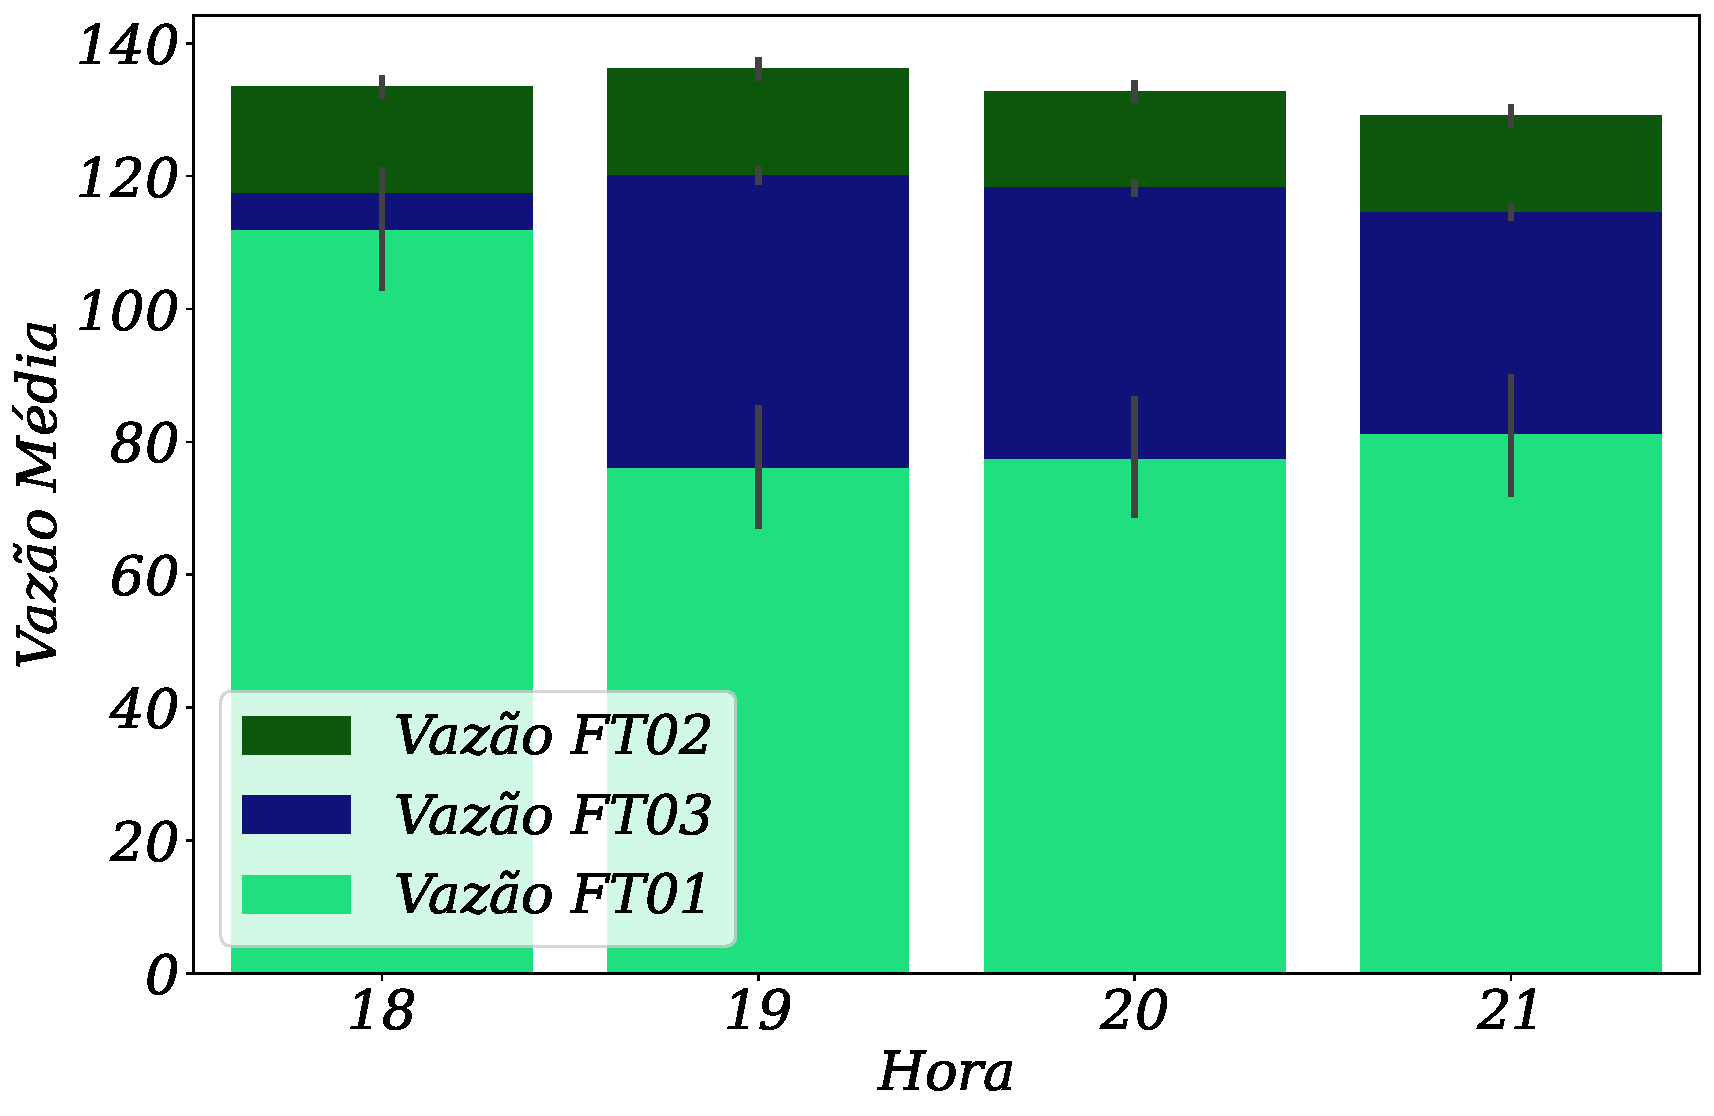
\includegraphics[width=0.9\linewidth]{Resultados/Figuras/grafico-barras-demanda}
	
	\label{fig:grafico-barras-demanda}
	
	\fonte{Elaboração própria a partir de dados da SANEPAR (2018 a 2020)}
\end{figure}

O gráfico de barras apresentado na Figura \ref{fig:grafico-barras-demanda} mostra a demanda média das variáveis de fluxo (Vazão de Entrada-FT01, Vazão de Gravidade-FT02 e Vazão de Recalque-FT03) durante o intervalo das 18h às 21h. Cada barra representa a média da demanda para cada variável em um horário específico dentro desse intervalo. A altura de cada barra indica a magnitude da demanda média para a respectiva variável. Essa visualização permite que sejam identificados os horários em que as variáveis de fluxo apresentaram maior demanda, o que é útil para o planejamento e gerenciamento adequado do sistema.

A questão de pesquisa \ref{q5}\ref{q5:c} foi respondida através da análise dos dados, permitindo a identificação dos horários de maior demanda durante o período das 18h às 21h. A tabela a seguir apresenta os resultados para as três variáveis estudadas: vazão de entrada-FT01, vazão de gravidade-FT02 e vazão de recalque-FT03.




\begin{table}[H]
	\centering
	\caption{Demanda de água}\label{tb:dem}
	\begin{tabular}{@{}ccc@{}}
		\toprule
		\textbf{Variável}         & \textbf{Horário de Maior Demanda} & \textbf{Valor da Demanda} \\ \midrule
		Vazão de entrada - FT01   & 2020/10/08 21:00:00               & $383,87 m^3/h$                   \\
		Vazão de gravidade - FT02 & 2020/10/20 18:00:00               & $326,17 m^3/h$                    \\
		Vazão de recalque - FT03  & 2020/11/26 19:00:00               & $194,35 m^3/h$                    \\ \bottomrule
	\end{tabular}
	
	
	\fonte{Elaboração própria a partir de dados da SANEPAR (2018 a 2020)}
\end{table}

Os resultados destacam os horários específicos em que cada variável apresentou maior demanda dentro do intervalo das 18h às 21h, fornecendo importantes para o planejamento e gerenciamento adequado do sistema. A tabela \ref{tb:dem} resume essas informações.


\eqref{q5}\ref{q5:d} Durante as horas de pico, é necessário que o nível do reservatório esteja mantido dentro na média de $3.9005 \ m^3$ para evitar o acionamento das bombas. Manter o nível do reservatório dentro dessa faixa permitirá que o sistema opere de forma eficiente, atendendo à demanda de água sem a necessidade de acionar as bombas.

\eqref{q5}\ref{q5:e} É importante destacar que a vazão de recalque exerce um impacto mais significativo no nível do reservatório em comparação com as outras vazões. Essa diferença se deve ao fato de que a vazão de recalque está diretamente relacionada à injeção de água no reservatório por meio da bomba localizada próxima à sua base. Em contraste, as demais vazões possuem alguns valores ausentes, o que limita sua influência na análise geral do sistema.







 




